\documentclass[12pt,a4paper]{report}

% ===================== PACKAGES =====================
\usepackage[utf8]{inputenc}
\usepackage[T1]{fontenc}
\usepackage[french]{babel}
\usepackage{amsmath,amssymb}
\usepackage{newpxtext}
\usepackage{newpxmath}
\usepackage{graphicx}
\usepackage[most]{tcolorbox}
\usepackage{xcolor}
\usepackage{colortbl}
\usepackage{tabularx}
\usepackage{titlesec}
\usepackage{fancyhdr}
\usepackage{geometry}
\usepackage{setspace}
\usepackage{ragged2e}
\usepackage{caption}
\usepackage{subcaption}
\usepackage{float}
\usepackage{booktabs}
\usepackage{longtable}
\usepackage{pdflscape}
\usepackage{hyperref}
\usepackage{etoc}
\usepackage{pgfornament} % pour le petit séparateur décoratif
\usepackage{enumitem}
\usepackage{eso-pic}   % pour dessiner la bordure pleine page
\usepackage{tikz}
\usepackage{pgfplots}
\pgfplotsset{compat=1.18}
\usetikzlibrary{calc}  % nécessaire pour les calculs de coordonnées ($(...)+(...)$)

\geometry{margin=2.5cm,headheight=16pt}
\setlength{\emergencystretch}{2em}

% ===================== COULEURS =====================
\definecolor{navyblue}{HTML}{1B365D}

% Puce sobre et professionnelle pour les éléments non numérotés
\newcommand{\professionalbullet}{%
  \tikz[baseline=-0.55ex]\fill[navyblue] (0,0) circle (2.2pt);%
}
\setlist[itemize,1]{
  label=\professionalbullet,
  leftmargin=1.8em,
  labelsep=0.65em,
  itemsep=0.25em,
  topsep=0.4em,
  parsep=0pt
}

% Encadré d'introduction inspiré du modèle fourni
\newtcolorbox{chapterintro}{
  enhanced,
  colback=navyblue!8,
  colframe=navyblue!45,
  boxrule=0.9pt,
  arc=2mm,
  left=10pt,
  right=10pt,
  top=8pt,
  bottom=8pt
}

% Mise en valeur homogène des principales formules méthodologiques
\newtcolorbox{formulabox}[2][0.80\linewidth]{
  enhanced,
  width=#1,
  center,
  colback=navyblue!3,
  colframe=navyblue,
  boxrule=1.5pt,
  arc=2mm,
  left=8pt,
  right=8pt,
  top=5pt,
  bottom=5pt,
  title={#2},
  fonttitle=\bfseries,
  coltitle=navyblue,
  attach title to upper={\par\smallskip}
}

% ===================== BORDURE DE PAGE (page de garde uniquement) =====================
% Dessine un cadre bleu marine proche des bords de la page.
\newcommand{\pageborder}{%
  \AddToShipoutPictureBG*{%
    \begin{tikzpicture}[remember picture,overlay]
      \draw[navyblue, line width=6pt]
        ($(current page.north west)+(0.5cm,-0.5cm)$) rectangle
        ($(current page.south east)+(-0.5cm,0.5cm)$);
    \end{tikzpicture}%
  }%
}

% ===================== EN-TETES =====================
\pagestyle{fancy}
\fancyhf{}
\renewcommand{\headrulewidth}{0.4pt}
\fancyhead[C]{\scriptsize\slshape \leftmark}
\fancyfoot[C]{\thepage}

% Style commun aux titres d'annexes, meme police et meme taille.
\newcommand{\annextitlefont}{\normalfont\LARGE\bfseries\color{navyblue}}

\titleformat{\chapter}[hang]
  {\normalfont\fontfamily{qcs}\selectfont\bfseries\color{navyblue}}
  {\raisebox{0pt}[0pt][0pt]{\begin{tikzpicture}[baseline=(current bounding box.center)]
     \node[fill=navyblue,minimum width=2.8cm,minimum height=2.8cm,inner sep=0pt] (chapterbox) {};
     \node[white,font=\itshape\small,anchor=north] at ([yshift=-2mm]chapterbox.north) {Chapitre};
     \node[white,font=\fontsize{40}{40}\selectfont,anchor=south] at ([yshift=1mm]chapterbox.south) {\thechapter};
   \end{tikzpicture}}}
  {0.7cm}
  {\large\setstretch{0.95}\raggedright\hyphenpenalty=10000\exhyphenpenalty=10000}
\titlespacing*{\chapter}{0pt}{-10pt}{24pt}

\titleformat{name=\chapter,numberless}[display]
  {\annextitlefont\hyphenpenalty=10000\exhyphenpenalty=10000}
  {}
  {0pt}
  {\raggedright}
  [\vspace{0.35em}{\color{navyblue}\titlerule[1.2pt]}]

\titleformat{\section}[hang]
  {\normalfont\large\bfseries\color{navyblue}\filright}
  {\colorbox{navyblue}{\makebox[1.45cm][c]{\color{white}\thesection}}}
  {0.45cm}
  {}
  [\vspace{-0.2em}{\color{navyblue}\titlerule[0.7pt]}]
\titleformat{\subsection}
  {\normalfont\large\bfseries\color{navyblue}\filright}{\thesubsection}{1em}{}
\titleformat{\subsubsection}
  {\normalfont\normalsize\bfseries\color{navyblue}\filright}{\thesubsubsection}{1em}{}
% Sous-titres de niveau inférieur, détachés du texte et sans numérotation.
\titleformat{\paragraph}[block]
  {\normalfont\small\bfseries\itshape\color{navyblue}\filright}{}{0pt}{}
\titlespacing*{\paragraph}{0pt}{1.5ex plus 0.5ex minus 0.2ex}{0.6ex}
\setcounter{secnumdepth}{3}
\setcounter{tocdepth}{3}

% Numérotation hiérarchique globale : Chapitre I, I.1, I.1.1, etc.
\renewcommand{\thechapter}{\Roman{chapter}}
\renewcommand{\thesection}{\thechapter.\arabic{section}}
\renewcommand{\thesubsection}{\thesection.\arabic{subsection}}
\renewcommand{\thesubsubsection}{\thesubsection.\arabic{subsubsection}}

\hypersetup{
    colorlinks=true,
    linkcolor=navyblue,
    citecolor=navyblue,
    urlcolor=navyblue,
}

\addto\captionsfrench{\renewcommand{\tablename}{Tableau}}
\newcommand{\tablesource}{%
  \par\vspace{1pt}%
  {\fontsize{8}{9}\selectfont\itshape Source : ANACIM, calculs de l'auteur\par}%
}

\title{Analyse des dynamiques climatiques et de leur variabilité à partir de la pluviométrie au Sénégal}
\author{ZONGO Abdoul Kader}
\date{Octobre 2026}

\begin{document}
\hypersetup{pageanchor=false}

% ===================== PAGE DE GARDE =====================
\begin{titlepage}
\pageborder
\centering
\vspace{0.8cm}
{\fontsize{15}{17}\selectfont\rmfamily\bfseries République du Sénégal}\\[0.15cm]

\includegraphics[width=2.2cm,height=1.7cm,keepaspectratio]{armoiries_senegal.png}\\[0.45cm]

{\fontsize{15}{17}\selectfont\rmfamily\bfseries Ministère de l'Économie, des Finances et du Plan (MEFP)}\\[0.15cm]

\includegraphics[width=3cm,height=1.35cm,keepaspectratio]{prism-uploads/image_16.png}\\[0.35cm]

{\fontsize{15}{17}\selectfont\rmfamily\bfseries Agence nationale de la Statistique et de la Démographie (ANSD)}\\[0.15cm]

\includegraphics[width=2.5cm,height=1.55cm,keepaspectratio]{prism-uploads/image_17.png}\\[0.25cm]

{\fontsize{15}{17}\selectfont\rmfamily\bfseries École nationale de la Statistique et de l'Analyse économique Pierre Ndiaye (ENSAE)}\\[0.15cm]

\includegraphics[width=2.2cm,height=1.55cm,keepaspectratio]{Logo_ENSAE.png.png}\\[0.55cm]

\begin{tcolorbox}[colback=navyblue,colframe=navyblue,arc=2pt,width=6cm,halign=center]
{\color{white}\large\bfseries Rapport de stage}
\end{tcolorbox}

\vspace{0.12cm}
\pgfornament[width=6cm]{88}\par
\vspace{0.18cm}

\begin{tcolorbox}[
  enhanced,
  colback=white,
  colframe=navyblue!55,
  boxrule=1pt,
  arc=1mm,
  title=THÈME,
  fonttitle=\large\bfseries,
  coltitle=white,
  attach boxed title to top center={yshift=-3mm},
  boxed title style={colback=navyblue,colframe=navyblue,sharp corners,boxrule=0pt,width=3cm,halign=center},
  top=7mm,
  bottom=4mm,
  interior style={top color=white,bottom color=navyblue!10},
  fuzzy shadow={1mm}{-1mm}{0mm}{0.2mm}{navyblue!25}
]
\centering
\textbf{\large ANALYSE DES DYNAMIQUES CLIMATIQUES ET DE LEUR VARIABILITÉ EN FONCTION DE LA PLUVIOMÉTRIE AU SÉNÉGAL}
\end{tcolorbox}

\vspace{0.45cm}
{\large\color{navyblue}\bfseries Rédigé par :}\\
 {\large\textbf{Abdoul Kader ZONGO}}\\
{\large\textit{\color{navyblue}Élève Ingénieur Statisticien Économiste (ISE1 Cycle Long)}}

\vspace{0.45cm}
{\large\color{navyblue}\bfseries Supervisé par :}\\
\begin{minipage}{0.7\textwidth}
\centering
{\large\textbf{M. Mouhamadou Bassirou DIOUF}}\\
{\large\textit{\color{navyblue}Comptable national}}
\end{minipage}

\vspace{0.55cm}
\begin{tcolorbox}[colback=navyblue!6,colframe=navyblue,arc=0pt,width=4.8cm,halign=center]
{\large\textbf{Novembre 2026}}
\end{tcolorbox}
\end{titlepage}
\hypersetup{pageanchor=true}

% Numérotation en chiffres romains pour tout le préliminaire (comme dans l'original : i à ix)
\pagenumbering{roman}

% ===================== DECHARGE =====================
\chapter*{DÉCHARGE}
\addcontentsline{toc}{chapter}{DÉCHARGE}
\markboth{DÉCHARGE}{DÉCHARGE}
\begin{tcolorbox}[
  enhanced,
  colback=white,
  colframe=navyblue,
  boxrule=1pt,
  arc=3mm,
  left=12pt,
  right=12pt,
  top=12pt,
  bottom=12pt,
  interior style={top color=white,bottom color=navyblue!8},
  fuzzy shadow={1.5mm}{-1.5mm}{0mm}{0.3mm}{navyblue!30}
]
\begin{justify}
L’Agence nationale de la Statistique et de la Démographie (ANSD) et l’École nationale de la Statistique et de l’Analyse économique Pierre Ndiaye (ENSAE) n’entendent donner aucune approbation ni improbation au sujet des opinions émises dans ce document. Elles doivent être considérées comme propres à l’auteur.
\end{justify}
\end{tcolorbox}

% ===================== REMERCIEMENTS =====================
\chapter*{REMERCIEMENTS}
\addcontentsline{toc}{chapter}{REMERCIEMENTS}
\markboth{REMERCIEMENTS}{REMERCIEMENTS}

Avant tout propos, nous tenons à exprimer notre profonde gratitude à tout le personnel de l’Agence nationale de la Statistique et de la Démographie (ANSD), en particulier à M. Abdou DIOUF, Directeur général de l’Agence, pour l’opportunité qui nous a été offerte d’effectuer ce stage au sein de cette institution.

Nos sincères remerciements à l'École nationale de la Statistique et de l'Analyse économique Pierre Ndiaye (ENSAE), pour la qualité de la formation reçue. Nous témoignons toute notre reconnaissance à son corps administratif et professoral, notamment au Dr. Idrissa DIAGNE, Directeur de l’ENSAE, au Dr. Mamadou BALDE, Directeur des Études et des Stages de l’ENSAE, à M. Thierno Ibrahima BARRY, Chef de la filière des Ingénieurs Statisticiens Économistes (ISE), au Dr. Alassane AW, Responsable de la filière des Analystes Statisticiens (AS), au Dr. Souleymane FOFANA, Chef de l’Unité de recherche de l’ENSAE ainsi qu’à M. Jean Jacques Roger FAYE, Responsable pédagogique de la classe ISE1 Cycle Long.

Nos remerciements à M. Malick DIOP, Chef de la Division de la Comptabilité nationale (DCN), pour son accueil chaleureux au sein de cette division, ainsi que pour ses nombreux conseils et ses orientations éclairées ; à Mme Ndeye Khoudia Laye SEYE, Chef du Bureau des Comptes annuels et sectoriels (BCAS) ; à M. Kandé CISSÉ, Chef du Bureau des Comptes trimestriels et régionaux (BCTR) et à Mme Iphygénie SARR, ancienne experte au BCAS. Nous remercions tous les membres, sans exception, de la Division de la Comptabilité nationale pour leur accueil chaleureux, leur appui constant, leur disponibilité et leurs précieux enseignements.

Nous tenons à exprimer une reconnaissance particulière à M. Mouhamadou Bassirou DIOUF, notre encadreur, pour son soutien, sa disponibilité, son dynamisme et ses conseils avisés, qui ont grandement contribué à la réussite de ce travail.

Enfin, nous témoignons notre gratitude à toutes les personnes qui, de près ou de loin, ont contribué à l'aboutissement de ce travail et qui, par leur soutien, leurs critiques constructives et leurs encouragements, ont facilité sa réalisation.

% ===================== AVANT-PROPOS =====================
\chapter*{AVANT-PROPOS}
\addcontentsline{toc}{chapter}{AVANT-PROPOS}
\markboth{AVANT-PROPOS}{AVANT-PROPOS}
L’École nationale de la Statistique et de l’Analyse économique Pierre Ndiaye (ENSAE) est un établissement d’enseignement supérieur rattaché à l’Agence nationale de la Statistique et de la Démographie (ANSD). Elle est membre du Réseau des Écoles de Statistiques africaines (RESA), avec l’École nationale de la Statistique et d’Économie Appliquée (ENSEA) d’Abidjan, l’Institut sous-régional de la Statistique et d’Économie appliquée (ISSEA) de Yaoundé et l’École nationale d’Économie appliquée et de Management (ENEAM) de Cotonou. La formation délivrée par l’ENSAE comprend plusieurs filières : les Ingénieurs de Travaux Statistiques (ITS), une formation de quatre ans achevée en 2023 ; les Analystes Statisticiens (AS), un programme de trois ans lancé en 2020 ; les Ingénieurs Statisticiens Économistes (ISE) en cycle court sur trois ans et en cycle long sur cinq ans, ce dernier ayant également commencé en 2020. S'ajoutent à ces programmes le Master Aide à la Décision et Évaluation des Politiques publiques (ADEPP) et le Master en Statistiques agricoles. Afin de garantir une formation de qualité, il est prévu que les élèves effectuent au moins un stage durant leur cursus. Ainsi, les élèves Ingénieurs statisticiens économistes cycle long réalisent un stage d’immersion à la fin de leur deuxième année d’études. Ce stage vise à les familiariser avec le milieu professionnel et leur offrir l’opportunité de mettre en pratique les connaissances théoriques acquises. Il aboutit à la rédaction d’un rapport de stage sur un thème spécifique, qui sera ensuite présenté lors d'une soutenance devant un jury. Le présent rapport, intitulé « Analyse des dynamiques climatiques et de leur variabilité en fonction de la pluviométrie au Sénégal » s’inscrit dans ce cadre et a été rédigé à l’issue d’un stage de deux (02) mois à l’Agence nationale de la Statistique et de la Démographie.

% ===================== SOMMAIRE =====================
\clearpage
\phantomsection
\addcontentsline{toc}{chapter}{SOMMAIRE}
\renewcommand{\contentsname}{SOMMAIRE}
% Le sommaire ne présente que les grandes parties du rapport.
\begingroup
\newlength{\sommairechapterindent}
\settowidth{\sommairechapterindent}{\bfseries CHAPITRE~IV~:\enspace}
\etocsetnexttocdepth{chapter}
\etocsetstyle{chapter}
  {}
  {}
  {\noindent
   \bfseries
   \etocifnumbered
     {\hangindent=\sommairechapterindent\hangafter=1%
      {\color{navyblue}CHAPITRE~\etocnumber{}~:}\enspace\etocname}
     {\hangindent=0pt\etocname}%
   \nobreak\dotfill\nobreak\makebox[2.5em][r]{\etocpage}\par
   \normalfont}
  {}
\tableofcontents
\endgroup

% ===================== SIGLES ET ACRONYMES =====================
\chapter*{LISTE DES SIGLES ET ACRONYMES}
\addcontentsline{toc}{chapter}{LISTE DES SIGLES ET ACRONYMES}
\markboth{LISTE DES SIGLES ET ACRONYMES}{LISTE DES SIGLES ET ACRONYMES}
\begingroup
\small
\setlength{\parindent}{0pt}
\setlength{\parskip}{0pt}
\newcommand{\sigleentry}[2]{%
  \par\noindent
  \hangindent=2.95cm\hangafter=1%
  \makebox[2.35cm][l]{\textbf{#1}}%
  \makebox[0.35cm][c]{:}%
  \hspace{0.12cm}#2\par\vspace{0.28em}%
}
\sigleentry{ANACIM}{Agence nationale de l'aviation civile et de la météorologie}
\sigleentry{ANSD}{Agence nationale de la Statistique et de la Démographie}
\sigleentry{BCAS}{Bureau des comptes annuels et sectoriels}
\sigleentry{BCTR}{Bureau des comptes trimestriels et régionaux}
\sigleentry{CAH}{Classification ascendante hiérarchique}
\sigleentry{CDN}{Contribution déterminée au niveau national}
\sigleentry{CDSE}{Cadre de développement des Statistiques de l'Environnement}
\sigleentry{CSE}{Centre de suivi écologique}
\sigleentry{DAMCP}{Direction des Aires marines communautaires protégées}
\sigleentry{DAPSA}{Direction de l'analyse, de la prévision et des statistiques agricoles}
\sigleentry{DCCTEFV}{Direction des changements climatiques, de la transition écologique et des financements verts}
\sigleentry{DCN}{Division de la Comptabilité nationale}
\sigleentry{DEFCCS}{Direction des eaux, forêts, chasses et conservation des sols}
\sigleentry{DGPRE}{Direction générale de la planification et des ressources en eau}
\sigleentry{DHORT}{Direction de l'horticulture}
\sigleentry{DIREC}{Direction de la réglementation et du contrôle}
\sigleentry{DPEE}{Direction de la prévision et des études économiques}
\sigleentry{DPN}{Direction des parcs nationaux}
\sigleentry{DSECN}{Direction des Statistiques Économiques et de la Comptabilité nationale}
\sigleentry{ERE}{Équilibres ressources-emplois}
\sigleentry{GIEC}{Groupe d'experts intergouvernemental sur l'évolution du climat}
\sigleentry{IPS}{Indice pluviométrique standardisé}
\sigleentry{IRD}{Institut de recherche pour le développement}
\sigleentry{ISRA}{Institut sénégalais de recherches agricoles}
\sigleentry{LPSE}{Lettre de politique du secteur de l'environnement}
\sigleentry{ONAS}{Office national de l'assainissement du Sénégal}
\sigleentry{ORSTOM}{Office de la recherche scientifique et technique outre-mer}
\sigleentry{PNA}{Plan national d'adaptation aux changements climatiques}
\sigleentry{PSD}{Plans stratégiques de développement}
\sigleentry{SCN}{Système de comptabilité nationale}
\sigleentry{SEEA}{System of Environmental Economic Accounting}
\sigleentry{SNDD}{Stratégie nationale de développement durable}
\sigleentry{SNDS}{Stratégie nationale de développement de la statistique}
\sigleentry{TRE}{Tableaux des ressources et emplois}
\sigleentry{ZCIT}{Zone de convergence intertropicale}
\endgroup

% ===================== LISTES =====================
\renewcommand{\listfigurename}{LISTE DES FIGURES}
\renewcommand{\listtablename}{LISTE DES TABLEAUX}
\renewcommand{\tablename}{Tableau}
\listoffigures
\addcontentsline{toc}{chapter}{LISTE DES FIGURES}
\listoftables
\addcontentsline{toc}{chapter}{LISTE DES TABLEAUX}
% ===================== RESUME =====================
\chapter*{RÉSUMÉ}
\addcontentsline{toc}{chapter}{RÉSUMÉ}
\markboth{RÉSUMÉ}{RÉSUMÉ}

Ce travail analyse l'évolution de la pluviométrie au Sénégal sur la période 1961-2025, à partir des cumuls pluviométriques annuels des quatorze régions du pays collectés au niveau de l'ANACIM. Si la rupture pluviométrique sahélienne de la fin des années 1960 fait l'objet d'un large consensus dans la littérature, sa caractérisation à l'échelle du Sénégal demeure fragmentée, les travaux existants portant le plus souvent sur des stations ou des bassins isolés et reposant sur une analyse temporelle univariée qui ne permet pas d'appréhender les relations entre régions. Cette étude vise ainsi à analyser l’évolution de la pluviométrie au Sénégal et à caractériser sa variabilité. Pour y parvenir, elle identifie les ruptures dans les séries pluviométriques régionales et en mesure l’ampleur, dégage les principales structures de variabilité entre les régions et met en évidence les grands régimes pluviométriques du pays en y classant les années grâce à la combinaison d’une approche univariée et d’une approche multivariée.

La démarche méthodologique associe quatre procédures complémentaires de détection des ruptures (test de \textsc{Pettitt}, statistique de \textsc{Buishand}, méthode bayésienne de \textsc{Lee} et \textsc{Heghinian}, segmentation de \textsc{Hubert}), une comparaison des moyennes avant et après rupture, une analyse en composantes principales (ACP), une classification ascendante hiérarchique (CAH) des années selon leur régime pluviométrique et un lissage temporel en utilisant le filtre passe-bas de Hanning d'ordre 2.

Les résultats mettent en évidence une rupture avérée pour huit des quatorze régions, organisée en deux périodes cohérentes avec la climatologie régionale : un déficit concentré entre 1966 et 1971 (baisses de 16\% à 32\%), et une reprise plus récente entre 1998 et 2007 (hausses d'environ 17\% à 23\%). L'ACP révèle un signal pluviométrique national dominant (54,6\% de la variance), complété par un contraste secondaire (8,4\%) entre l’Est et le Sud, d’une part, et l’Ouest, d’autre part. La classification qui en découle dégage trois régimes, à savoir les régimes sec, normal et humide, dont la répartition chronologique recoupe étroitement les ruptures identifiées, la classe normale s'apparentant davantage à une zone de transition qu'à un régime pleinement distinct.

Ces résultats rejoignent le consensus établi par la littérature sur la sécheresse sahélienne, tout en apportant une lecture combinée, temporelle et spatiale, de la variabilité pluviométrique récente au Sénégal. L'étude souligne enfin la nécessité de renforcer le réseau d'observation pluviométrique et d'intégrer l'analyse infra-annuelle des précipitations dans les travaux futurs.

\medskip
\noindent\textbf{Mots-clés : pluviométrie ; Sénégal ; rupture climatique ; variabilité spatiale ; analyse en composantes principales ; classification ascendante hiérarchique ; Sahel.}

% ===================== ABSTRACT =====================
\chapter*{ABSTRACT}
\addcontentsline{toc}{chapter}{ABSTRACT}
\markboth{ABSTRACT}{ABSTRACT}
\selectlanguage{english}

This study analyzes the evolution of rainfall in Senegal over the period 1961-2025, based on annual rainfall totals for the fourteen regions provided by ANACIM. While the Sahelian rainfall shift of the late 1960s is now the subject of broad scientific consensus, its characterization at the scale of Senegal remains fragmented, as existing studies have mostly focused on individual stations or watersheds and relied on univariate temporal analyses that do not capture the relationships between regions. This study therefore aims to analyse the evolution of rainfall in Senegal and to characterise its variability. To this end, it identifies the shifts in regional rainfall series and measures their magnitude, brings out the main structures of variability across regions, and highlights the country’s main rainfall regimes by classifying the years within them, combining a univariate approach with a multivariate one.

The methodological approach combines four complementary shift-detection procedures (the \textsc{Pettitt} test, the \textsc{Buishand} statistic, the Bayesian method of \textsc{Lee} and \textsc{Heghinian}, and \textsc{Hubert} segmentation), a comparison of means before and after the shift, a principal component analysis (PCA), an agglomerative hierarchical clustering (AHC) of years according to their rainfall regime, and a temporal smoothing using a second-order Hanning low-pass filter.

The results reveal a confirmed shift in eight of the fourteen regions, organized into two periods consistent with regional climatology: a deficit concentrated between 1966 and 1971 (decreases of 16\% to 32\%), and a more recent recovery between 1998 and 2007 (increases of approximately 17\% to 23\%). The PCA reveals a dominant national rainfall signal (54.6\% of variance), complemented by a secondary contrast (8.4\%) between the East and South, on the one hand, and the West, on the other. The resulting classification identifies three regimes, namely dry, normal, and wet, whose chronological distribution closely matches the identified shifts, with the normal class appearing more as a transition zone than as a fully distinct regime.

These results are consistent with the established consensus in the literature on the Sahelian drought, while providing a combined temporal and spatial reading of recent rainfall variability in Senegal. The study further highlights the need to strengthen the rainfall observation network and to incorporate sub-annual analysis of precipitation in future research.

\medskip
\noindent\textbf{Keywords: rainfall; Senegal; rainfall shift; spatial variability; principal component analysis; agglomerative hierarchical clustering; Sahel.}
\selectlanguage{french}

% ===================== INTRODUCTION =====================
% On mémorise la dernière page en chiffres romains du préliminaire
% pour pouvoir reprendre cette numérotation après le corps du rapport (Bibliographie, Annexe).
\newcounter{frontmatterpage}
\setcounter{frontmatterpage}{\value{page}}

\clearpage
\pagenumbering{arabic}
\chapter*{INTRODUCTION}
\addcontentsline{toc}{chapter}{INTRODUCTION}
\markboth{INTRODUCTION}{INTRODUCTION}
Au cours des dernières décennies, le changement climatique s’est imposé comme l’un des grands défis de notre époque, ses effets se manifestant avec une ampleur croissante à l’échelle mondiale. Selon le sixième rapport d'évaluation du GIEC (2021), la température moyenne à la surface du globe a augmenté d'environ 1,1°C entre la période 1850-1900 et 2011-2020, avec un réchauffement plus marqué sur les continents. Cette évolution s'accompagne d'une intensification de plusieurs phénomènes extrêmes tels que les vagues de chaleur, les sécheresses, les inondations et la montée du niveau de la mer, qui rappellent que le changement climatique ne se résume pas à une hausse des températures : il affecte tout autant le cycle de l'eau et, par conséquent, la disponibilité et la répartition des ressources en eau. Cette dimension hydrique revêt une importance particulière dans les régions où les activités économiques et les conditions de vie demeurent étroitement dépendantes du climat. À sa suite, l'économiste Nicholas Stern souligne qu'une grande partie des dommages liés au changement climatique provient de l'eau, ou de son absence, à travers les sécheresses, les inondations et les tempêtes. Dans cette perspective, l'étude des précipitations constitue une entrée privilégiée pour analyser les dynamiques climatiques régionales, celles-ci conditionnant directement la disponibilité de l'eau, le fonctionnement des écosystèmes et les activités humaines qui en dépendent.

Cette problématique est particulièrement sensible en Afrique de l'Ouest, où l'agriculture pluviale, l'élevage et l'accès aux ressources en eau restent étroitement liés à la pluviométrie. Le régime des précipitations est ainsi l'un des principaux facteurs de la productivité alimentaire dans la région du Sahel (Sarr et al., 2013). La région sahélienne a notamment connu, à partir de la fin des années 1960, l'un des épisodes de sécheresse les plus marqués du XXe siècle. Les travaux de Nicholson (1983), Lamb (1982), Hulme (1992) ainsi que de Le Barbé et Lebel (1997) ont largement documenté la rupture pluviométrique observée autour de 1968-1972, qui s'est accompagnée d'un déplacement des isohyètes\footnote{Une isohyète est une ligne reliant sur une carte les points qui reçoivent la même quantité de précipitations sur une période donnée. Le déplacement des isohyètes vers le sud traduit un assèchement du climat.} vers le sud. La durée de cette sécheresse et la date de la reprise pluviométrique ont toutefois fait débat dans la littérature. Certains travaux situent sa persistance jusqu'à la fin des années 1990 (L'Hôte et al., 2002), tandis que d'autres identifient une reprise dès le milieu de cette décennie (Ozer et al., 2003 ; Ali et Lebel, 2009). Plus récemment, plusieurs études mettent en évidence une recrudescence de la variabilité pluviométrique et des événements extrêmes en Afrique de l'Ouest (Sarr et al., 2015).

Le Sénégal, situé à l’extrémité occidentale du Sahel, s’inscrit pleinement dans cette dynamique régionale. En effet, son économie et les moyens d’existence d’une part importante de sa population demeurent sensibles aux fluctuations pluviométriques. Selon le RGPH-5, 44,5\% des ménages sont agricoles et 91\% d’entre eux pratiquent une agriculture pluviale (ANSD, 2025). Le pays a connu, comme une grande partie du Sahel, un déficit pluviométrique durable à partir de la fin des années 1960 - en 1972, la station de Dakar n'a par exemple enregistré que 117mm de précipitations, contre une médiane de 500mm (Dacosta et al., 2002). Cette période sèche s'est prolongée pendant plusieurs décennies avant qu'une reprise des précipitations ne soit observée à partir des années 2000. Cette reprise n'a cependant pas été uniforme sur l'ensemble du territoire : Bodian (2014) relève des déficits compris entre 12\% et 24\% selon les stations, lorsqu'on compare les périodes antérieure et postérieure à la rupture. Ces évolutions montrent que la pluviométrie sénégalaise se caractérise à la fois par une forte variabilité temporelle et par des disparités spatiales importantes. Une augmentation récente des cumuls annuels ne signifie d'ailleurs pas nécessairement un retour au régime pluviométrique antérieur à la période sèche : les transformations en cours peuvent tout aussi bien concerner la variabilité interannuelle, la répartition spatiale des précipitations ou la fréquence des épisodes pluvieux. L'analyse des seules moyennes apparaît dès lors insuffisante pour rendre compte de l'ensemble de ces dynamiques.

Si la datation de la rupture pluviométrique sahélienne de la fin des années 1960 fait aujourd'hui l'objet d'un large consensus dans la littérature scientifique, la caractérisation de la variabilité pluviométrique récente au Sénégal demeure plus fragmentée. Les travaux empiriques consacrés au pays ont principalement porté sur des stations, des bassins versants ou des régions particulières, permettant de mettre en évidence des évolutions temporelles et des différences spatiales, mais sans toujours proposer une lecture d'ensemble du territoire national. Sur le plan méthodologique, les travaux existants ont largement recours aux méthodes statistiques de détection des ruptures et d'analyse des tendances pour identifier les changements intervenus dans les séries pluviométriques. Ces approches permettent notamment de repérer une modification significative du comportement d'une série et d'en comparer les niveaux avant et après une rupture. Toutefois, l'analyse d'une série prise isolément renseigne principalement sur son évolution temporelle et reste limitée lorsqu'il s'agit d'appréhender simultanément les relations entre plusieurs régions. Compléter l'analyse temporelle des séries par une approche multivariée, permettant de considérer conjointement les différentes dimensions spatiales de la pluviométrie, prend alors tout son sens : c'est cette combinaison d'outils statistiques complémentaires qui peut permettre de passer de l'identification de changements ponctuels à une caractérisation plus globale de la variabilité pluviométrique au Sénégal.

Dès lors, une question centrale émerge : comment la pluviométrie a-t-elle évolué au Sénégal au cours du temps, et quelle forme prend sa variabilité ? Cette interrogation conduit aux questions spécifiques suivantes : à quelle date se situent les éventuelles ruptures dans les séries pluviométriques régionales sénégalaises et quelle est leur ampleur ? Quelles sont les principales structures de la variabilité pluviométrique entre les régions du Sénégal ? Quels sont les grands régimes pluviométriques qui caractérisent le pays, et comment les années se répartissent-elles selon ces régimes ?

C’est ainsi que cette étude vise à analyser l’évolution de la pluviométrie au Sénégal et à caractériser sa variabilité. Plus spécifiquement, il s’agira d’identifier les ruptures dans les séries pluviométriques régionales et d’en mesurer l’ampleur, de dégager les principales structures de variabilité entre les régions et de mettre en évidence les grands régimes pluviométriques du pays en y classant les années.

En cohérence avec les objectifs de recherche fixés ci-dessus, quatre hypothèses sont formulées. La première suppose l'existence d'une rupture statistiquement significative dans les séries pluviométriques régionales au Sénégal. La deuxième fait l'hypothèse d'une différence significative entre les moyennes pluviométriques calculées avant et après cette rupture. La troisième repose sur l'existence de régimes pluviométriques traduisant une hétérogénéité spatiale du territoire national. Enfin, la quatrième avance qu'une typologie cohérente des années sèches, humides et de transition peut être dégagée à partir de ces régimes. Ces hypothèses sont formulées à partir de la littérature sur la sécheresse sahélienne, de la configuration climatique du pays et des objectifs de l’étude.

Afin de tester les hypothèses de recherche et d’atteindre les objectifs fixés, cette étude adopte une approche quantitative fondée sur l’analyse statistique des séries pluviométriques régionales. Elle a pour but d’identifier objectivement les évolutions spatiales et temporelles. La démarche combine quatre étapes complémentaires : la détection des ruptures, la comparaison des moyennes avant et après rupture, l’analyse en composantes principales (ACP) pour synthétiser la variabilité entre régions, et la classification des années selon les régimes ainsi obtenus. Les données mobilisées concernent les cumuls pluviométriques annuels des quatorze régions du Sénégal, fournis par l'ANACIM.

Dans l’optique d’apporter une réponse claire à notre problématique, ce rapport est structuré en quatre chapitres. Le premier consistera en la présentation de la structure d’accueil et au bilan des activités réalisées. Le cadre conceptuel et la revue de la littérature feront l’objet du deuxième chapitre. Quant au troisième chapitre, il sera question de présenter les données utilisées ainsi que les différentes méthodes mobilisées pour réaliser ce travail. Enfin, nous procéderons au dernier chapitre à une analyse des dynamiques climatiques, en détectant les ruptures dans les séries pluviométriques régionales et en dégageant, par une analyse en composantes principales, les régimes climatiques du pays.

% ===================== CHAPITRE 1 =====================
\chapter{PRÉSENTATION DE LA STRUCTURE D'ACCUEIL ET BILAN DES ACTIVITÉS}

\begin{chapterintro}
\begin{justify}
Ce chapitre présente l'Agence nationale de la Statistique et de la Démographie (ANSD), structure d'accueil du stage, à travers son historique, ses missions et son organisation. Il décrit ensuite le dispositif des statistiques environnementales au Sénégal, avant de dresser le bilan des principales activités réalisées durant le stage.
\end{justify}
\end{chapterintro}

\vspace{0.45cm}
\noindent{\color{navyblue}\rule{\textwidth}{1.1pt}}
\vspace{0.35cm}

\section{Présentation de la structure d'accueil (ANSD)}

\subsection{Historique et missions de l'ANSD}
Créée en 2004 par la loi N° 2004-21 du 12 juillet 2004 portant organisation des activités statistiques, l'ANSD est une structure administrative dotée de la personnalité juridique et d'une autonomie de gestion placée sous tutelle du ministre chargé de la statistique et sous gouvernance d'un Conseil de Surveillance. Elle est dirigée par un Conseil de Surveillance de représentants de la Primature, du Ministère de l'Économie, des Finances et du Plan, de la Banque Centrale des États de l'Afrique de l'Ouest (BCEAO), des organisations patronales, des centrales syndicales des travailleurs et des centres de recherche universitaire. Elle a comme organe de direction exécutive la Direction générale dont le Directeur général et le Directeur général adjoint sont, tous deux, nommés par décret. Son rôle est d'assurer la cohésion technique des différentes activités du Système Statistique National (SSN) et de veiller, par la même, à la production et la diffusion des données statistiques. Ces dernières serviront d'appui au Gouvernement, aux administrations publiques, de même qu'au secteur privé et aux partenaires au développement.

La mission de l'ANSD s'articule autour des points suivants :
\begin{itemize}[nosep]
\item veiller à l'élaboration et à la mise en œuvre des programmes pluriannuels et annuels de statistique ;
\item assurer la mise en application des méthodes, concepts, définitions, normes, classifications et nomenclatures approuvés par le Comité technique des programmes statistiques ;
\item préparer les dossiers à soumettre aux réunions du Conseil national de la statistique et du Comité technique des programmes statistiques ;
\item assurer le secrétariat et l'organisation des réunions du Conseil national de la statistique et du Comité technique des programmes statistiques ainsi que de ses sous-comités sectoriels ;
\item réaliser des enquêtes d'inventaire à couverture nationale notamment les recensements généraux de la population et ceux des entreprises ;
\item produire les comptes nationaux ;
\item suivre la conjoncture et la prévision économiques en rapport avec le service en charge de la prévision et de la conjoncture économique ;
\item élaborer et gérer les fichiers des entreprises et des localités ;
\item élaborer les indicateurs économiques, sociaux et démographiques ;
\item centraliser et diffuser les synthèses des données statistiques produites par l'ensemble du système statistique national ;
\item favoriser le développement des sciences statistiques et la recherche économique appliquée relevant de sa compétence ;
\item promouvoir la formation du personnel spécialisé pour le fonctionnement du système national d'information statistique par l'organisation des cycles de formation appropriés notamment au sein d'une école à vocation régionale ou sous-régionale intégrée à l'agence.
\end{itemize}

Dans les différentes régions, l'ANSD est représentée par 14 Services régionaux de la Statistique et de la Démographie (SRSD) qui sont sous la Direction de l'Action Régionale (DAR) chargée de gérer le personnel, le matériel et les moyens financiers des services tout en coordonnant et animant le système statistique régional.

\subsection{Organisation de l'agence}
La Direction générale comprend le Directeur général, le Directeur général adjoint, les Conseillers techniques, l'Auditeur interne, la Cellule du Contrôle de gestion, la Cellule de passation des marchés, la Cellule de communication, la Cellule juridique, la Cellule de gestion des partenariats, le Service de sécurité, le Service médical et les secrétariats du Directeur général et du Directeur général adjoint. Un Bureau de l'archivage et du courrier y est rattaché pour la gestion des archives et des courriers à l'arrivée et au départ de l'Agence. En dehors de la direction générale, l'ANSD compte 8 directions à savoir :
\begin{itemize}[nosep]
\item la DSECN (Direction des Statistiques économiques et de la Comptabilité nationale) ;
\item la Direction des Statistiques démographiques et sociales (DSDS) ;
\item la Direction des Systèmes d'Information et de la Diffusion (DSID) ;
\item la Direction de l'Administration Générale et des Ressources Humaines (DAGRH) ;
\item la Direction de l’École nationale de la Statistique et de l’Analyse économique (ENSAE) ;
\item la Direction de la Méthodologie, de la Coopération statistique et de l'Innovation (DMCI) ;
\item la Direction de l’Action régionale (DAR) ;
\item l'Agence Comptable.
\end{itemize}

\subsection{Direction des Statistiques économiques et de la Comptabilité nationale (DSECN)}

La Direction des Statistiques économiques et de la Comptabilité nationale (DSECN) est responsable de la production des statistiques sur les entreprises, des statistiques économiques et conjoncturelles, ainsi que des comptes nationaux. Elle a également pour vocation de mener des études et des recherches ciblées sur des thématiques spécifiques liées à l'économie. Elle est structurée en trois divisions principales.

\subsubsection{Division des Statistiques économiques (DSE)}

La Division des Statistiques économiques (DSE) assure la gestion des systèmes d'information statistique relatifs aux entreprises et la création d'outils tels que :
\begin{itemize}[nosep]
\item la Banque de Données économiques et financières (BDEF) ;
\item le suivi de la démographie des entreprises ;
\item la gestion du Répertoire national des Entreprises et Associations (RNEA) ;
\item la gestion du Numéro d'Identification nationale des Entreprises et Associations (NINEA) ;
\item le fonctionnement du Centre unique de Collecte de l'Information (CUCI).
\end{itemize}

Elle est organisée autour de trois bureaux :
\begin{itemize}[nosep]
\item le Bureau des Répertoires (BR) ;
\item le Bureau des Statistiques d'Entreprises (BSE) ;
\item le Bureau des Statistiques sectorielles (BSS).
\end{itemize}

\subsubsection{Division des Statistiques conjoncturelles (DSC)}

La Division des Statistiques conjoncturelles (DSC) est chargée des enquêtes de conjoncture menées auprès des entreprises, ainsi que de l'élaboration des statistiques sur le commerce extérieur et des indicateurs conjoncturels. Elle est structurée en trois bureaux :
\begin{itemize}[nosep]
\item le Bureau des Enquêtes de Conjoncture (BEC) ;
\item le Bureau des Échanges extérieurs (BEE) ;
\item le Bureau des Prix (BP).
\end{itemize}

\subsubsection{Division de la Comptabilité nationale (DCN)}

La Division de la Comptabilité nationale (DCN), la Division des Statistiques économiques et la Division des Statistiques conjoncturelles sont les trois divisions de la DSECN.

La DCN produit et analyse l'ensemble des comptes nationaux en synthétisant les statistiques et les indicateurs que produisent les autres unités de l'ANSD ou les organismes extérieurs compétents. Elle élabore les tableaux de synthèse des comptes nationaux, notamment les comptes de production, les Tableaux des Ressources et Emplois (TRE) à prix courants et constants, les comptes des administrations publiques et privées, les équilibres macroéconomiques ainsi que les comptes des institutions financières.

La DCN contribue à l'établissement des budgets économiques en collaboration avec la Direction de la Prévision et des Études économiques (DPEE) et d'autres institutions, comme la Douane, la Banque Centrale des États de l'Afrique de l'Ouest (BCEAO) et la Comptabilité publique. Elle réalise également des études macroéconomiques et thématiques. Elle comprend deux bureaux : le Bureau des Comptes annuels et sectoriels (BCAS) et le Bureau des Comptes trimestriels et régionaux (BCTR).

\begin{itemize}[leftmargin=1.8em,label=\professionalbullet,itemsep=1.2em]
\item \textbf{\color{navyblue}Bureau des Comptes annuels et sectoriels (BCAS)}\par\smallskip
Le Bureau des Comptes annuels et sectoriels (BCAS) exploite les données des principaux secteurs de l'économie, tels que l'agriculture, l'industrie, le commerce, les services et le secteur informel, afin d'élaborer les comptes nationaux annuels. Il établit les comptes de production par secteur et veille à l'équilibre entre les ressources et les emplois des produits concernés.

Il participe à la production des comptes des administrations publiques, des entités privées et des institutions financières. Conformément au Système de Comptabilité nationale (SCN), il contribue également à l'élaboration des tableaux de synthèse économique, notamment les comptes de branche, les équilibres ressources-emplois, les Tableaux des Ressources et Emplois (TRE) et le Tableau des Comptes économiquement intégrés (TCEI).

Le BCAS veille enfin à l'application des normes internationales de comptabilité nationale afin de garantir la qualité, la cohérence et la comparabilité des comptes produits.

\item \textbf{\color{navyblue}Bureau des Comptes trimestriels et régionaux (BCTR)}\par\smallskip
Le Bureau des Comptes trimestriels et régionaux (BCTR), anciennement Bureau des Synthèses et Études Analytiques (BSEA), notre bureau d’accueil, est l’un des deux bureaux de la Division de la Comptabilité nationale. Il est chargé de l’élaboration et de l’analyse des comptes nationaux trimestriels ainsi que des comptes régionaux.

À ce titre, le BCTR contribue à la production d’indicateurs permettant de suivre l’évolution infra-annuelle de l’activité économique et d’apprécier la répartition territoriale de la création de richesse. Il centralise, traite, harmonise et analyse les données nécessaires à l’estimation du PIB trimestriel et des agrégats économiques régionaux.

Aussi, il réalise des études et analyses approfondies à caractères macroéconomiques ou thématiques, en collaboration avec le Ministère de l’Économie des Finances et du Plan et les services compétents de l’ANSD.

Le BCTR veille également à la cohérence de ses estimations avec les comptes nationaux annuels et au respect des normes internationales en matière de comptabilité nationale.
\end{itemize}

\section{Dispositif des statistiques environnementales au Sénégal}

\subsection{Cadre institutionnel et réglementaire}

Le Sénégal dispose d'un cadre politique relativement étoffé en matière d'environnement, structuré autour de plusieurs textes et stratégies. Il s'agit, entre autres, de la loi sur la biosécurité, du Code de l'environnement, du Code forestier, de la Lettre de Politique du Secteur de l'Environnement (LPSE), de la Contribution déterminée au niveau national (CDN), du Plan national d'Adaptation aux changements climatiques (PNA) et de la Stratégie nationale de Développement durable (SNDD). Sur le plan statistique, la loi de 2012 relative à l'organisation et à la coordination du Système statistique national (SSN) confie à l'ANSD la coordination technique de l'ensemble du dispositif, tandis que la Stratégie nationale de Développement de la Statistique (SNDS IV, 2024-2028) affirme la volonté de l'État de renforcer la production et la qualité des statistiques environnementales. Ce cadre reste toutefois incomplet : aucune stratégie n'est encore spécifiquement dédiée aux statistiques de l'environnement, ce qui limite leur place explicite dans le pilotage des politiques publiques.

\subsection{Organisation et acteurs de la production des statistiques environnementales}

Le Système statistique national (SSN) sénégalais est coordonné par l'ANSD avec l'implication de l'ensemble des structures publiques productrices de données. Cependant, il n'existe pas encore de cadre national de statistiques de l'environnement formellement institué. La production repose principalement sur l'ANSD et sur plusieurs directions techniques du Ministère de l'Environnement et de la Transition écologique, ainsi que sur diverses structures sectorielles intervenant dans les domaines de l'eau, de l'agriculture, de la météorologie, de l'assainissement, de la recherche et de la gestion des ressources naturelles.

Certaines de ces structures disposent d'unités, de cellules ou de divisions chargées du suivi-évaluation ou de la production statistique. Nous pouvons notamment citer le Centre de Suivi écologique (CSE), la Direction des Aires Marines Communautaires Protégées (DAMCP), la Direction des Parcs Nationaux (DPN), la Direction des Eaux, Forêts, Chasses et Conservation des Sols (DEFCCS), la Direction de la Réglementation et du Contrôle (DIREC), ainsi que la Direction des Changements Climatiques, de la Transition écologique et des Financements Verts (DCCTEFV). À ces structures s'ajoutent des acteurs sectoriels tels que l'ANACIM, la Direction générale de la Planification et des Ressources en Eau (DGPRE), l'Office national de l'Assainissement du Sénégal (ONAS), l'Institut sénégalais de Recherche agricole (ISRA), l'Institut national de Pédologie (INP), la Direction de l'Analyse, de la Prévision et des Statistiques agricoles (DAPSA) et la Direction de l'Horticulture (DHORT). Cette organisation permet la production d'un important volume d'informations environnementales, mais demeure caractérisée par une forte dispersion institutionnelle et par l'absence de mécanisme permanent dédié à la coordination entre ces différents producteurs.

\subsection{Sources et référentiels des statistiques environnementales}

La production des statistiques environnementales au Sénégal repose sur des sources de nature variée. Il s'agit d'abord de données administratives issues des déclarations, permis et contrôles effectués par des structures sectorielles, telles que les autorisations environnementales, le suivi forestier ou la gestion des déchets. Ces données sont complétées par des enquêtes et des recensements ponctuels menés notamment par l'ANSD, à l'image du Recensement général de la Population, de l'Habitat, de l'Agriculture et de l'Élevage (RGPHAE) de 2013 ou de l'Enquête agricole annuelle ainsi que la réalisation des comptes économiques et environnementaux.

S'y ajoutent les observations directes des réseaux de stations météorologiques et hydrologiques, gérés respectivement par l'ANACIM et la DGPRE, ainsi que, de manière croissante, des données issues de la télédétection et de l'imagerie satellitaire, mobilisées par des structures comme le Centre de Suivi écologique pour le suivi du couvert végétal et des écosystèmes. Sur le plan méthodologique, le Cadre de développement des Statistiques de l'Environnement des Nations Unies (CDSE) constitue le principal référentiel international auquel ces différentes sources peuvent être rattachées, bien que son appropriation reste encore partielle au niveau national.

\subsection{Place des données climatiques et pluviométriques dans le dispositif statistique}

Au sein de ce dispositif, les données climatiques occupent une place particulière du fait de leur ancienneté et de leur relative continuité. Leur production relève du mandat propre de l'Agence Nationale de l'Aviation Civile et de la Météorologie (ANACIM), qui constitue la seule structure habilitée à exploiter le réseau national d'observation météorologique et à collecter, contrôler et archiver les données climatologiques officielles du pays.

Parmi ces données, les observations pluviométriques occupent une position centrale : elles sont recueillies quotidiennement par un réseau de stations synoptiques et de postes pluviométriques répartis sur l'ensemble du territoire national, puis transmises, contrôlées et consolidées en séries annuelles au niveau du service climatologique de l'ANACIM. Ces données alimentent des usages variés, notamment les bulletins agrométéorologiques, les alertes climatiques et le suivi des campagnes agricoles. Elles constituent également une ressource scientifique de premier plan pour l'analyse du climat sur le long terme.

La pluviométrie fait partie des variables environnementales pour lesquelles on dispose de séries longues, qui permettent d’étudier son évolution sur plusieurs décennies. C’est sur ces données, collectées et conservées par l’ANACIM, que s’appuie l’ensemble du présent travail.

\subsection{Contraintes et défis du dispositif}

L'évaluation du dispositif met en évidence plusieurs contraintes institutionnelles qui freinent le développement des statistiques environnementales au Sénégal. La première tient à l'absence d'un cadre institutionnel formellement consacré à leur coordination. En effet, il n'existe ni système national dédié, ni stratégie sectorielle spécifique, ni comité permanent de coordination, ce qui constitue une faiblesse structurelle du dispositif actuel.

À cela s'ajoutent des difficultés de collaboration interinstitutionnelle, liées au manque de ressources nécessaires à l'organisation de rencontres techniques régulières, au temps insuffisant consacré aux activités relatives aux statistiques environnementales et aux chevauchements de responsabilités entre les structures. Par ailleurs, l'absence de protocoles formels d'échange de données et de mécanismes institutionnalisés de concertation peut accentuer la fragmentation des initiatives et la dispersion des informations environnementales entre les différents producteurs.

Toutes ces contraintes se traduisent globalement par des besoins persistants en matière de renforcement des capacités, de financement, de transfert de compétences et d'amélioration des dispositifs de production des données. Ces limites se retrouvent concrètement dans les données pluviométriques mobilisées pour ce travail, dont la couverture spatiale et la profondeur temporelle demeurent inégales selon les régions.

\section{Bilan des activités réalisées}

Le bilan de notre stage s’articule autour de deux volets essentiels : d’une part, l’immersion au sein de la Division de la Comptabilité nationale ; d’autre part, la rédaction du présent rapport.

\subsection{Immersion}

L'immersion de huit semaines effectuée au sein de la Division de la Comptabilité nationale a constitué pour nous une expérience formatrice dans l'univers des comptes nationaux. Elle nous a permis de découvrir les rouages du monde professionnel qui contribue au fonctionnement de l'activité économique du pays. Dès notre arrivée, nous avons reçu une documentation afin de nous familiariser avec les concepts et les méthodes en vigueur qui guident les comptables nationaux dans la réalisation de leur tâche. Au fil du stage, d'autres documents nous ont été transmis pour approfondir notre compréhension des activités en cours et faciliter notre participation active.

Durant le stage, nous avons eu l'occasion de participer à plusieurs activités, parmi lesquelles :

Une présentation devant les membres du Bureau des Comptes Trimestriels et Régionaux sur l'estimation du commerce intra-zone dans un pays a été réalisée le 18 août 2026. Ce travail de recherche, qui nous a été confié, nous a permis d'approfondir nos connaissances en économie. L'idée était d'examiner, dans un pays africain comme le Sénégal, la manière dont se fait la modélisation et l'estimation du commerce intranational. Ce travail nous a permis de retracer, à travers la littérature, les différents modèles de gravité (standard, structurel, panel, VAR, calibré) utilisés pour ce type de problème, de formaliser l'équation gravitationnelle et ses variables explicatives, puis de confronter les résultats afin d'en tirer des enseignements de politique économique. Les experts du BCTR ont apprécié ce travail de recherche et nous ont recommandé une certaine prudence quant aux hypothèses d'application de ces modèles au contexte sénégalais. Ils nous ont par ailleurs encouragés à approfondir la réflexion sur ce sujet.

Ensuite, nous avons pris part, dans le cadre du processus d’élaboration des comptes de 2025, à l’étape du pré-arbitrage portant sur l’estimation de la consommation finale des ménages. Cette phase s’est appuyée sur un cadre méthodologique fondé sur les principes de la comptabilité nationale et sur les déterminants économiques de la demande. La consommation finale des ménages constitue l’une des principales composantes de la demande finale dans les comptes nationaux. Son estimation revêt une importance particulière en raison de sa contribution à la mesure du produit intérieur brut, à l’analyse de la demande intérieure et à l’évaluation des conditions de vie des populations. Cette étape, la deuxième du genre dans ce processus, permet de vérifier la cohérence et l’exhaustivité des données collectées et traitées. Elle permet également de déceler d’éventuels décalages entre l’année en cours et l’année précédente.

Par ailleurs, le lundi 28 septembre 2026, nous avons eu l'insigne honneur de participer au sein de l'ANSD à l'atelier de validation des résultats des comptes nationaux du deuxième trimestre de 2026. En effet, la publication des travaux de mise à jour des comptes annuels et sectoriels du Sénégal et de leur alignement a franchi une étape majeure le mardi 25 novembre 2025. Avec pour année de base 2021, cette opération du \textit{rebasing} a permis d'intégrer de nouveaux secteurs clés, d'actualiser les nomenclatures et de réévaluer les indicateurs globaux. Ainsi, il était nécessaire, à la suite, d'initier les travaux de rétropolation et d'alignement des comptes trimestriels sur la nouvelle année de base 2021. Cela permet d'améliorer la qualité des prévisions pour alimenter les ERE et de garantir la cohérence des comparaisons temporelles sectorielles. Cet atelier a fait l'objet de riches échanges afin d'améliorer la qualité des résultats et a conduit à la publication du rapport final sur ces travaux.

Enfin, les réunions de suivi des activités de division nous ont permis de produire des comptes rendus de réunion, mettant ainsi en application les connaissances acquises dans le cours de technique d'expression durant l'année académique. En plus de ces réunions de division, nous avons rédigé un compte rendu d'une réunion consacrée à la préparation de l'atelier de lancement du CDSE au Sénégal.

Le stage a permis de renforcer plusieurs valeurs professionnelles, notamment le sérieux dans le travail, la collaboration et l'esprit d'équipe, gages de meilleurs résultats, ainsi que l'assiduité et la ponctualité.

\subsection{Rédaction du rapport}

Après avoir reçu notre thème de stage, une première réunion avec le maître de stage nous a permis de mettre en place le planning de rédaction du rapport. Cette étape cruciale nous a permis de mieux nous organiser afin d'achever la rédaction dans les meilleurs délais. Une deuxième réunion nous a ensuite permis d'avoir un aperçu sur les comptes économiques et environnementaux, de mieux comprendre le CDSE, le CSE, la CDN, le SEEA et plus largement le fonctionnement et l'organisation des statistiques environnementales au Sénégal. Des réunions régulières ont également été organisées avec notre encadreur pour faire le point sur l'état d'avancement du rapport, occasion de recevoir ses observations sur le travail accompli. C'est dans ce cadre que la base de données sur les cumuls pluviométriques de l'ensemble des régions du Sénégal nous a été transmise ; elle est issue de l'Agence Nationale de l'Aviation Civile et de la Météorologie (ANACIM).

En définitive, le stage effectué au sein de l'une des divisions de l'ANSD, service officiel de production et de diffusion des statistiques du Sénégal, a été une expérience enrichissante à plusieurs égards. Il nous a permis de mettre en pratique les connaissances acquises au cours de notre formation académique, tout en nous plongeant dans la réalité du monde professionnel.

% ===================== CHAPITRE 2 =====================
% Chapitre 2 adapté du fichier Word corrigé fourni par l'auteur.
% Le tableau récapitulatif de la revue théorique et empirique est volontairement exclu.

\newcommand{\concept}[1]{%
  \par\medskip\noindent
  \professionalbullet\hspace{0.65em}%
  {\color{navyblue}\bfseries #1}%
  \par\nobreak\smallskip
}

\chapter{CADRE CONCEPTUEL ET REVUE DE LITTÉRATURE}

\begin{chapterintro}
\begin{justify}
Ce chapitre a pour objectif de préciser les principaux concepts nécessaires à la compréhension des dynamiques climatiques et de la variabilité pluviométrique. Il propose ensuite une revue des contributions théoriques et empiriques consacrées à l'évolution des précipitations, aux ruptures climatiques et aux régimes pluviométriques, afin de situer l'étude dans la littérature existante.
\end{justify}
\end{chapterintro}

\vspace{0.45cm}
\noindent{\color{navyblue}\rule{\textwidth}{1.1pt}}
\vspace{0.35cm}

\section{Cadre conceptuel}

\subsection{Climat}

Le mot « climat » vient du grec « klima », qui signifie « inclinaison ». Étymologiquement, il désigne la hauteur du Soleil en un lieu et à une saison donnée, traduisant l'ancrage originel de la climatologie dans l'observation astronomique plutôt que météorologique.

Le climat désigne également la synthèse statistique des conditions atmosphériques observées en un lieu donné sur une période de référence, généralement fixée à trente ans par l’Organisation météorologique mondiale (OMM, 2018). Il fait ainsi référence à l'état moyen de l'atmosphère, incluant la température, la pluviométrie, l'humidité et le vent. Il se distingue en cela du temps, qui renvoie à l'état instantané de l'atmosphère à un moment donné. Cet état moyen, considéré dans sa globalité, constitue le point de départ des définitions plus spécifiques présentées ci-après.

\subsection{Dynamique climatique}

La dynamique climatique désigne l'ensemble des processus physiques qui régissent le fonctionnement du climat à travers les échanges d'énergie entre l'atmosphère, l'océan et la surface continentale (GIEC, 2021). Elle se distingue ainsi de la simple description statistique du climat évoquée précédemment : alors que celui-ci renvoie à un état moyen, la dynamique climatique s'intéresse aux mécanismes qui produisent cet état et ses variations.

Dans l'espace sahélien, elle renvoie principalement au fonctionnement de la mousson ouest-africaine, dont l'établissement saisonnier commande l'essentiel du régime pluviométrique national, ainsi qu'aux mouvements de grande échelle de l'atmosphère et des océans, qui régulent les transferts de chaleur entre les basses et les hautes latitudes.

\concept{La circulation atmosphérique générale}
Elle représente le mouvement organisé des masses d'air à l'échelle planétaire sous l'effet du réchauffement inégal de la Terre entre l'équateur et les pôles. Ce déséquilibre thermique engendre des cellules de convection\footnote{Cellule de convection : C'est une circulation en boucle où l’air chaud s’élève, se refroidit en altitude puis redescend.}, dont la cellule de Hadley, qui achemine l'air chaud et humide de l'équateur vers les tropiques, où il redescend en formant les hautes pressions subtropicales caractéristiques des zones désertiques.

\concept{La zone de convergence intertropicale (ZCIT)}
Elle désigne la bande de basses pressions située près de l’équateur, où convergent les alizés des deux hémisphères. L’air chaud et humide s’y élève, ce qui produit une forte nébulosité et des précipitations abondantes. Elle se déplace avec le Soleil : plus au nord pendant l’été, plus au sud pendant l’hiver. Au Sénégal, sa remontée vers le nord de juin à septembre apporte la saison des pluies.

\concept{La mousson ouest-africaine}
Elle correspond au mécanisme saisonnier d'inversion des vents et des flux d'humidité, associé au déplacement de la zone de convergence intertropicale (ZCIT) entre les deux hémisphères. Son installation, généralement entre juin et septembre au Sénégal, commande la quasi-totalité des précipitations annuelles enregistrées sur le territoire.

\concept{Les interactions océan--atmosphère}
Elles désignent les échanges de chaleur et d'humidité entre la surface océanique et l'atmosphère, qui modulent la circulation atmosphérique tropicale. Les océans, en stockant et en restituant la chaleur avec une forte inertie, influencent la trajectoire des systèmes pluvieux bien au-delà de leurs propres limites géographiques.

\concept{Le forçage climatique}
Il représente toute perturbation, externe ou interne au système climatique, susceptible de modifier son équilibre énergétique (GIEC, 2021). Il peut être d'origine astronomique, radiative, océanique ou anthropique. Autrement dit, tout élément capable de perturber les entrées ou les sorties d'énergie du système climatique constitue un forçage climatique, qu'il s'agisse d'une modification du rayonnement solaire reçu, de la composition de l'atmosphère ou des échanges océan--atmosphère.

\subsection{Variabilité climatique}

La variabilité climatique désigne les fluctuations naturelles du climat autour de sa valeur moyenne, à des échelles de temps variées (Hulme, 1992). Elle concerne aussi bien des échelles courtes, telles que les saisons ou les années, que des échelles plus longues, de l'ordre de la décennie. Le GIEC (2021) précise que cette variabilité renvoie à la variance interne à l'intérieur d'un même régime climatique. Une phase sèche prolongée peut ainsi relever d'une simple variabilité interne du système climatique sahélien, sans traduire nécessairement une modification durable de ses paramètres moyens.

Cette variabilité trouve son origine dans trois grandes sources. D’abord, une variabilité naturelle externe, liée à des forçages extérieurs au système climatique tels que le forçage solaire, les cycles de Milankovitch ou le volcanisme. Ensuite, une variabilité naturelle interne, propre aux rétroactions internes du système climatique, notamment le couplage océan--atmosphère (ENSO, NAO, circulation thermohaline)\footnote{\textit{ENSO} : El Niño--Oscillation australe. C’est un phénomène couplé océan--atmosphère du Pacifique tropical qui alterne, de façon irrégulière, entre une phase chaude (El Niño) et une phase froide (La Niña). \textit{NAO} : Oscillation nord-atlantique. Il désigne la fluctuation de la différence de pression entre l’anticyclone des Açores et la dépression d’Islande, qui module les vents et les perturbations sur l’Atlantique Nord. \textit{Circulation thermohaline} : C’est la circulation océanique de grande échelle, engendrée par les différences de densité des eaux (température et salinité), qui transporte la chaleur entre les basses et les hautes latitudes.}. Enfin, une variabilité anthropique externe, résultant des activités humaines, à travers la perturbation de l'effet de serre et des conditions de surface.

On distingue notamment les formes suivantes.

\concept{La variabilité interannuelle}
Elle correspond à la succession d’années excédentaires et déficitaires en précipitations, d’une année à l’autre. Cette forme de variabilité est particulièrement marquée dans le régime climatique sahélien, où l’écart entre l’année la plus pluvieuse et l’année la plus sèche d’une même série peut dépasser 700mm.

\concept{La variabilité décennale}
Elle désigne l'alternance de phases pluriannuelles globalement sèches ou humides, telle que la longue période de déficit pluviométrique observée au Sahel entre la fin des années 1960 et le début des années 2000.

\subsection{Changement climatique}

Le changement climatique désigne une modification durable de l’état du climat, identifiable par des changements de sa moyenne et/ou de sa variabilité, qui persiste sur une longue période, généralement plusieurs décennies ou plus (GIEC, 2021). Il se distingue ainsi de la variabilité climatique, qui correspond aux fluctuations naturelles et à plus court terme autour de cet état moyen.

Ces modifications, qui durent généralement plusieurs décennies, se traduisent par des tendances progressives ou par des ruptures statistiques dans les séries observées. Le changement climatique peut résulter de forçages naturels, tels que les variations de l'activité solaire ou volcanique, ou de forçages anthropiques, au premier rang desquels figure l'augmentation des concentrations atmosphériques de gaz à effet de serre. L'influence de ces derniers sur le climat contemporain est aujourd'hui documentée avec un niveau de confiance élevé par les rapports successifs du GIEC.

Alors que la variabilité climatique renvoie à des fluctuations réversibles autour d'un état moyen stable, le changement climatique implique le passage à un nouvel état d'équilibre, sans garantie que le système revienne à sa configuration antérieure. Une rupture statistiquement significative ne suffit donc pas, à elle seule, à établir l'existence d'un changement climatique au sens strict du terme.

\subsection{Régime pluviométrique et indicateurs de mesure}

Le régime pluviométrique désigne les caractéristiques de la répartition saisonnière des précipitations en un lieu donné (OMM, 2012). Il détermine la durée et l’intensité des saisons sèches et humides. Au Sénégal, l’hivernage, qui s’étend généralement de juin à octobre, constitue la principale saison des pluies. Le pays présente un gradient pluviométrique national marqué, la pluviométrie moyenne annuelle augmentant du nord vers le sud (Touré et al., 2022). La pluviométrie, expression la plus concrète et la plus directement mesurable des concepts précédents, constitue la variable d’observation retenue dans le présent travail, à travers ses cumuls annuels. Par extension, on désigne ici par « régimes pluviométriques », les grands états pluviométriques interannuels (années sèches, normales et humides) qui se dégagent de l’analyse.

\concept{Les systèmes convectifs de méso-échelle (SCM)}
Ce sont de vastes ensembles d'orages organisés qui génèrent l'essentiel des précipitations en zone sahélienne. Les lignes de grains\footnote{Ligne de grains : ligne d’orages organisés en bande, accompagnée de vents et de pluies intenses au passage.}, caractérisées par un front convectif linéaire\footnote{Front convectif linéaire : Alignement d’orages formés par convection (ascension de l’air chaud et humide) et qui se déplace sous forme de bande.} pouvant s'étendre sur plusieurs centaines de kilomètres, en constituent l'exemple le plus typique en Afrique de l'Ouest.

\concept{L’indice d’aridité}
Il évalue le degré de sécheresse d’un milieu en comparant les précipitations annuelles à la température ou à l’évapotranspiration potentielle. Les indices de De Martonne et de Gaussen figurent parmi les plus couramment mobilisés dans la caractérisation climatique de l’Afrique de l’Ouest.

\paragraph{Indice de De Martonne}
L’indice de De Martonne est calculé selon la formule :

\begin{formulabox}[0.42\linewidth]{}
\[
I = \frac{P}{T+10}
\]
\end{formulabox}

Dans cette formule, $P$ désigne la précipitation totale annuelle, exprimée en mm, et $T$ la température moyenne annuelle, exprimée en °C. De Martonne a étudié la relation entre la valeur de cet indice et le type de végétation observé afin de caractériser le climat général d’une région.

\begin{table}[H]
\centering
\captionsetup{justification=centering,font=small,labelfont=bf}
\caption{Classes climatiques associées à l’indice d’aridité de De Martonne}
\label{tab:classes-indice-de-martonne}
\begingroup
\footnotesize
\renewcommand{\arraystretch}{1.18}
\setlength{\tabcolsep}{4pt}
\begin{tabularx}{\linewidth}{>{\centering\arraybackslash}p{1.7cm}>{\raggedright\arraybackslash}p{2.3cm}>{\raggedright\arraybackslash}p{3cm}X}
\toprule
\rowcolor{navyblue}
\color{white}\textbf{Valeur de $I$} &
\color{white}\textbf{Type de climat} &
\color{white}\textbf{Végétation potentielle} &
\multicolumn{1}{>{\centering\arraybackslash}X}{\color{white}\textbf{Exemples}} \\
\midrule
\rowcolor{navyblue!7}
0 à 5 & Hyperaride & Désert absolu & Vallée de la Mort (États-Unis) \\
5 à 10 & Aride & Désert & Désert du Sahara ; désert de l’Arizona (États-Unis) \\
\rowcolor{navyblue!7}
10 à 20 & Semi-aride & Steppe & Sahel, Kalahari \\
20 à 30 & Semi-humide & Prairie naturelle, forêt & Région parisienne, Orléans, région de Marseille \\
\rowcolor{navyblue!7}
30 à 40 & Humide & Forêt & Région de Lille \\
40 à 55 & Humide & Forêt & Rouen, Dieppe, Alençon \\
\bottomrule
\end{tabularx}
\endgroup
\par\smallskip
{\footnotesize\itshape Source : tableau fourni par l’auteur.}
\end{table}

\paragraph{Indice de Gaussen ou indice ombrothermique}
L’indice de Gaussen compare, mois par mois, les précipitations $P$ (en mm) à deux fois la température moyenne $T$ (en °C). D’après F. Bagnouls et H. Gaussen (1953), un mois est considéré comme sec lorsque ses précipitations sont inférieures ou égales à deux fois sa température moyenne, soit :

\begin{formulabox}[0.30\linewidth]{}
\[
P \leq 2T
\]
\end{formulabox}

Dans cette relation, $P$ désigne les précipitations du mois et $T$ sa température moyenne. Bagnouls et Gaussen ont développé le diagramme ombrothermique pour représenter cette comparaison au cours de l’année.


\concept{Le cumul pluviométrique et le nombre de jours de pluie}
Le cumul pluviométrique mesure la quantité totale de précipitations reçues sur une période donnée, qu'elle soit mensuelle, saisonnière ou annuelle. Le nombre de jours de pluie dénombre, quant à lui, les jours au cours desquels un seuil minimal de précipitation a été enregistré. La confrontation de ces deux indicateurs permet de nuancer l'interprétation d'un simple cumul : une pluviométrie stable ou en hausse, combinée à une baisse du nombre de jours pluvieux, signale une intensification des événements plutôt qu'un retour pur et simple aux conditions antérieures.

\section{Revue de littérature}

\subsection{Revue théorique}

Trois approches structurent la littérature sur les dynamiques climatiques et leur variabilité pluviométrique au Sénégal : la théorie des interactions océan--atmosphère, la théorie du bilan radiatif et de l'effet de serre, ainsi que l'approche statistique de détection des ruptures et des tendances. Ces approches ne sont pas concurrentes, mais complémentaires, chacune éclairant une dimension différente du problème tout en présentant ses propres limites.

\subsubsection{Théorie des interactions océan--atmosphère}

Cette théorie analyse les échanges de chaleur entre les océans et l'atmosphère. En raison de leur forte inertie thermique, les océans stockent la chaleur sur de longues périodes et influencent la trajectoire des vents et des systèmes pluvieux bien au-delà de leur emprise géographique propre. Appliquée au Sahel, cette approche a été formalisée par Folland, Palmer et Parker (1986), qui montrent que les phases sèches et humides observées dans la bande sahélienne sont fortement liées à des configurations contrastées des températures de surface des océans à l'échelle quasi mondiale. Ces anomalies thermiques marines provoquent des déplacements de la zone de convergence intertropicale et, par conséquent, des variations directes du régime pluviométrique régional.

Une déclinaison complémentaire, développée par Charney (1975), introduit une échelle plus locale en postulant un mécanisme de rétroaction entre la végétation, le sol et l'atmosphère. La dégradation du couvert végétal augmenterait l'albédo\footnote{Albédo : C'est une fraction du rayonnement solaire incident réfléchie par une surface, comprise entre 0 et 1. L’albédo d’un sol dépend de sa couleur, de son humidité et de son couvert végétal.} des sols, provoquerait une subsidence atmosphérique et réduirait les précipitations. Cette interprétation, longtemps mobilisée pour expliquer la sécheresse sahélienne par les pratiques agricoles locales, a depuis été nuancée par des travaux montrant que la rétroaction positive entre la végétation et les pluies relèverait davantage d'un recyclage local de l'humidité que du seul effet d'albédo initialement avancé.

\subsubsection{Théorie du bilan radiatif et de l'effet de serre}

Le climat dépend de l'équilibre entre l'énergie solaire reçue par la Terre et l'énergie qu'elle réémet vers l'espace sous forme de rayonnement infrarouge. L'effet de serre naturel, dû à la présence de gaz atmosphériques tels que la vapeur d'eau et le dioxyde de carbone, permet de maintenir une température moyenne d'environ 15°C à la surface du globe, contre une valeur théorique négative en son absence. Cette théorie, dont les fondements remontent aux travaux de Tyndall (1861), puis d'Arrhenius (1896), établit que toute augmentation de la concentration atmosphérique en gaz à effet de serre rompt l'équilibre radiatif et entraîne un réchauffement global. Elle constitue le socle théorique du changement climatique anthropique contemporain, tel que documenté par les rapports successifs du GIEC.

Ce réchauffement agit directement sur le cycle de l'eau. D'après la relation de Clausius-Clapeyron, la capacité de l'atmosphère à contenir de la vapeur d'eau augmente d'environ 7\% par degré de réchauffement. Plus d'humidité disponible alimente plus d'énergie latente dans les systèmes convectifs, d'où l'hypothèse d'une intensification du cycle hydrologique : évaporation accrue, précipitations plus intenses lors des événements pluvieux, et contrastes plus marqués entre périodes humides et périodes sèches (Held et Soden, 2006 ; Trenberth, 2011). Cette intensification n'est toutefois pas uniforme dans l'espace. En Afrique de l'Ouest, la pluie dépend aussi de la mousson, des températures de surface océanique et de la position de la zone de convergence intertropicale (Nicholson, 2013). Le signal radiatif peut donc se combiner à la variabilité régionale, ou la masquer.

Cette théorie permet de formuler l'hypothèse suivante selon laquelle une partie des changements observés dans le régime pluviométrique du Sénégal pourrait s'inscrire dans cette dynamique globale, plutôt que résulter de la seule variabilité naturelle régionale.

\subsubsection{Approche statistique de détection des ruptures et des tendances}

Cette approche ne propose pas un mécanisme causal, mais fournit un ensemble d’outils permettant de caractériser objectivement la variabilité observée dans une série chronologique. Inspirée des travaux fondateurs de Lamb (1982) sur les indices d’anomalies, puis formalisée en climatologie par Hulme (1992) et Ozer, Bodart et Tychon (2005), elle repose sur des tests de rupture (Pettitt 1979, Buishand 1982, Hubert et al. 1989, Lubès-Niel et al. 1998) ainsi que sur des tests de tendance, tel que celui de Mann–Kendall.

Ces outils permettent d’identifier les changements de régime et les évolutions tendancielles au sein des séries climatiques, tout en offrant un cadre statistique adapté à l’analyse de leur variabilité. Cette approche présente toutefois une limite fondamentale largement reconnue dans la littérature : elle demeure essentiellement descriptive, dans la mesure où elle permet d’identifier l’existence, la localisation ou l’évolution d’un changement dans une série pluviométrique sans expliquer les mécanismes physiques ou climatiques qui en sont à l’origine.

\subsection{Revue empirique}

L'étude des dynamiques climatiques au Sénégal a donné lieu à un nombre croissant de travaux empiriques qui peuvent être regroupés en trois ensembles. Le premier porte sur la rupture pluviométrique de la fin des années 1960, le deuxième documente la reprise pluviométrique partielle des années 2000 et le troisième analyse les répercussions hydrologiques et écologiques de cette variabilité.

Les études empiriques montrent de façon convergente l'existence d'une rupture pluviométrique majeure à la fin des années 1960 au Sénégal. Diop (2023) met en évidence, à l’aide de la segmentation de Hubert, les principales ruptures d’une série longue de 122 ans, couvrant la période 1901–2022 au Sénégal et en Gambie. Il établit que les sécheresses du début des années 1970 et 1980 demeurent exceptionnelles au regard de l’ensemble de la période étudiée. Il confirme également le caractère représentatif des années 1968 et 2005 dans l’évolution de la pluviométrie nationale.

Touré et al. (2022), à partir de dix stations réparties sur l'ensemble du territoire sénégalais et couvrant la période 1960-2010, mobilisent plusieurs outils statistiques complémentaires : le test séquentiel de Mann--Kendall, le test de Van Belle et Hughes et le test régional de Mann--Kendall. Ils ne détectent qu'une seule tendance significative à la baisse, à la station de Matam. Ce résultat traduit un comportement globalement irrégulier de la pluviométrie sur le reste du territoire depuis 1960.

Bodian (2014), à partir d'un échantillon de 22 stations couvrant la période 1940-2013, confirme l'existence de cette rupture en appliquant trois méthodes de détection : le test de \textsc{Pettitt}, la méthode de \textsc{Lee} et \textsc{Heghinian} et la segmentation de \textsc{Hubert}. L'auteur conclut que le déficit pluviométrique persistait encore à la fin de la période étudiée, malgré les années humides ponctuelles de 1994 et 1999. Sagna et al. (2015) situent plus précisément cette rupture entre 1966 et 1969, l'année 1968 constituant le point de bascule le plus fréquemment retenu. Gaye (2017), sur les séries de Saint-Louis, Podor et Matam couvrant la période 1954-2013, aboutit à une conclusion similaire. La rupture est située en 1968 et jusqu'à 33 des 60 années étudiées se révèlent déficitaires selon les stations considérées.

Faye (2019), dans une étude consacrée à la région de Dakar entre 1960 et 2013, à l’aide du test de \textsc{Pettitt}, du test de Mann–Kendall et des indices de tendance et de variation, ne détecte aucune tendance pluviométrique statistiquement significative sur l’ensemble de la période, malgré une diminution de 211mm, soit 36,2\%, des totaux pluviométriques observés à partir de 1969. Ce résultat illustre la différence entre une rupture ponctuelle et une tendance linéaire. La même étude relève parallèlement une rupture thermique nette en 1994, accompagnée d'une augmentation de 0,9°C de la température moyenne entre les sous-périodes 1960-1994 et 1995-2013. Le réchauffement local ne suit donc pas nécessairement le même calendrier que l'évolution des précipitations.

Depuis la fin des années 1990, la pluviométrie sahélienne montre une amélioration partielle, avec l'apparition de plusieurs années excédentaires à partir de 2005. Cette reprise, documentée notamment par Gaye (2017), ne signifie cependant pas un simple retour aux conditions antérieures à 1968. Mendy (2023), à partir de la série centennale de Dakar-Yoff, confirme ce retour pluviométrique tout en soulignant qu'il coïncide avec une recrudescence des inondations urbaines dans l'agglomération dakaroise. Cela suggère une intensification des événements pluvieux plutôt qu'une simple réversibilité du régime antérieur. Cette interprétation rejoint les résultats obtenus à l'échelle nationale par Diop (2023), qui relève une diminution du nombre de jours de pluie malgré la reprise des cumuls. La sécheresse persisterait ainsi sous une forme différente de celle des décennies 1970-1990.

Un dernier ensemble de travaux documente les répercussions hydrologiques et écologiques de cette variabilité climatique, avec des résultats qui convergent avec ceux obtenus sur la pluviométrie. Dans le delta du fleuve Sénégal, Ngom (2013), en mobilisant les mêmes méthodes de détection de rupture que Bodian (2014), montre que la sécheresse a fortement réduit les écoulements naturels du fleuve. La régulation assurée par les barrages de Diama et de Manantali a depuis partiellement sécurisé l’approvisionnement en eau douce de la basse vallée.

Plus au sud, Faye (2017) analyse les débits du bassin de la Falémé à l'aide du test de Mann--Kendall appliqué aux séries mensuelles et annuelles couvrant la période 1954-2014. Son analyse révèle une baisse statistiquement significative des écoulements, atteignant 50\% à 59\% selon les stations de Fadougou, Gourbassi et Kidira. Ce résultat corrobore, au moyen d'un indicateur indépendant, l'ampleur de la péjoration pluviométrique documentée par ailleurs.

Sur la frange littorale des Niayes, les travaux d'Aguiar (2009) mettent en évidence une diminution progressive de la nappe phréatique côtière consécutive à la baisse des précipitations, favorisant une intrusion saline responsable du dépérissement du palmier à huile et d'autres espèces sensibles à la salinité des sols. Plus récemment, Sow et al. (2025), dans le sud du pays, relient directement la variabilité pluviométrique à la dégradation du couvert végétal de la forêt classée de Pata, à partir d'une analyse combinant données pluviométriques et imagerie satellitaire Landsat. Cette étude élargit la littérature récente de la seule mesure statistique vers l'étude des répercussions environnementales concrètes.

\enlargethispage{5\baselineskip}
En résumé, les revues théorique et empirique mettent en lumière la complexité des dynamiques climatiques et de leur variabilité pluviométrique au Sénégal. La revue théorique montre que cette variabilité trouve son explication dans l'articulation entre les forçages océaniques de grande échelle, l'équilibre radiatif global du système climatique et les outils statistiques qui permettent d'objectiver les ruptures observées dans les séries de données. Ces trois approches se complètent sans qu'aucune ne suffise isolément à rendre compte du phénomène.

La revue empirique fait ressortir un consensus autour de la rupture pluviométrique de la fin des années 1960, confirmée par des indicateurs aussi variés que les précipitations, les débits fluviaux et la dynamique du couvert forestier. Certains aspects demeurent toutefois discutés, notamment la nature exacte de la reprise pluviométrique amorcée dans les années 2000 et l'ampleur de la rupture selon les stations considérées. Les résultats apparaissent contrastés selon les zones étudiées et les méthodes mobilisées. Ces divergences soulignent l'importance de prendre en compte l'hétérogénéité spatiale et méthodologique dans l'analyse de la variabilité pluviométrique au Sénégal.
% ===================== CHAPITRE 3 =====================
\chapter{PRÉSENTATION DES DONNÉES ET APPROCHE MÉTHODOLOGIQUE}

\begin{chapterintro}
\begin{justify}
Ce chapitre a pour objectif de présenter les données pluviométriques mobilisées pour ce travail. Il expose ensuite l'approche méthodologique retenue pour étudier les dynamiques climatiques, notamment la détection des ruptures, la comparaison des moyennes, l'analyse en composantes principales et la classification des années selon les régimes pluviométriques.
\end{justify}
\end{chapterintro}

\vspace{0.45cm}
\noindent{\color{navyblue}\rule{\textwidth}{1.1pt}}
\vspace{0.35cm}

\section{Présentation des données}

\subsection{Source des données}

Les données pluviométriques mobilisées dans ce travail proviennent de l’Agence nationale de l’Aviation civile et de la Météorologie (ANACIM), structure nationale chargée de la collecte et de la diffusion des données climatologiques officielles au Sénégal. Elles concernent les cumuls pluviométriques annuels des quatorze régions du pays.

\subsection{Période et zone d'étude}

Les séries disponibles couvrent des périodes variables selon les régions, certaines débutant dès 1941, d'autres en 1950 ou 1961, toutes se prolongeant jusqu'en 2025. Les données ont été contrôlées et sont utilisées sur une période commune de 1961 à 2025 afin d'assurer leur comparabilité. Cette période comprend 65 années sans valeur manquante pour aucune des quatorze régions retenues. Cette durée dépasse largement les 30 ans minimum recommandés par l'Organisation météorologique mondiale pour établir des normales climatiques fiables. Elle couvre aussi trois phases clés : la période humide antérieure à la sécheresse, la rupture de la fin des années 1960-1970, et la reprise pluviométrique amorcée entre 1998 et 2007. Cette profondeur temporelle favorise ainsi l'identification et la caractérisation des ruptures.

Sur le plan spatial, l'étude couvre les quatorze régions du pays, selon un gradient nord--sud : du domaine sahélien (Matam, Louga, Saint-Louis) au domaine soudanien (Kolda, Sédhiou, Ziguinchor, Kédougou), en passant par les zones de transition du centre et de l'ouest (Dakar, Kaolack, Diourbel, Fatick, Thiès, Kaffrine, Tambacounda). Cette couverture permet ainsi d’étudier la variabilité pluviométrique à l’échelle nationale et de comparer les régions entre elles.

\subsection{Nature et structure des données pluviométriques}

Les données sont fournies sous la forme d’un classeur Excel structuré en plusieurs feuilles, chacune correspondant à une région. Chaque feuille se compose de deux colonnes : l’année d’observation et le cumul pluviométrique annuel, exprimé en mm, sans agrégation infra-annuelle (mensuelle ou décadaire). L’analyse portera donc sur la variabilité interannuelle des cumuls, à l’échelle régionale.

\section{Méthodologie de l'étude}

La démarche méthodologique débute par une analyse descriptive des séries pluviométriques régionales, suivie de quatre approches complémentaires : la détection des ruptures dans les séries chronologiques, la comparaison des moyennes avant et après la date de rupture, l'analyse en composantes principales et la classification des années selon les régimes pluviométriques.

\subsection{Statistique descriptive des séries pluviométriques régionales}

Une analyse descriptive est d’abord réalisée afin de caractériser les séries pluviométriques régionales. Elle repose sur des indicateurs de tendance centrale et de dispersion, tels que la moyenne interannuelle, l’écart-type et le coefficient de variation, complétés par les valeurs minimale et maximale. Ces indicateurs permettent d’apprécier le niveau moyen des précipitations ainsi que leur variabilité interannuelle. À cela s’ajoutent les coefficients d’asymétrie (skewness) et d’aplatissement (kurtosis), qui renseignent respectivement sur la symétrie et la forme de la distribution des précipitations.

L’évolution temporelle des précipitations est ensuite examinée à l’aide de l’indice pluviométrique standardisé (IPS). Développé par Lamb (1982), cet indice exprime l’écart de la pluviométrie annuelle d’une région à sa moyenne interannuelle, rapporté à son écart-type. La période de référence retenue pour la standardisation est 1961-2025. L’IPS est calculé comme suit :

\begin{formulabox}[0.40\linewidth]{}
\[
\mathrm{IPS}_i = \frac{x_i-\bar{x}}{s}
\]
\end{formulabox}

\noindent où $x_i$ désigne le cumul pluviométrique de l'année $i$, $\bar{x}$ la moyenne et $s$ l'écart-type de la série sur la période de référence 1961-2025. Une valeur positive de l'IPS traduit une année excédentaire, une valeur négative une année déficitaire, l'ampleur de l'écart étant exprimée en nombre d'écarts-types par rapport à la normale. L'indice pluviométrique standardisé moyen, calculé comme la moyenne des IPS des quatorze régions pour chaque année, permet de suivre la dynamique d'ensemble du régime pluviométrique national.

Pour faciliter la lecture visuelle de ces séries à l’échelle régionale, un lissage par filtre passe-bas de Hanning d’ordre 2 est ponctuellement appliqué en complément des figures brutes. Il s’agit d’un simple outil de représentation graphique, sans incidence sur les tests statistiques présentés dans les sections suivantes. Les poids utilisés sont 0,06 ; 0,25 ; 0,38 ; 0,25 ; 0,06. Pour le traitement de bord, les formules de bord du filtre de Hanning sont appliquées aux deux premières et aux deux dernières observations de chaque série.

\subsection{Méthode de détection des ruptures dans les séries chronologiques}

Une rupture se définit comme un changement dans la loi de probabilité des variables aléatoires dont les réalisations successives constituent la série chronologique étudiée (Lubès et al., 1994). Autrement dit, elle se traduit par un changement brutal et durable le long d'une série de précipitations. Sa détection repose sur des méthodes statistiques choisies pour la robustesse de leurs fondements théoriques. Ces méthodes visent principalement à repérer un changement dans la moyenne de la série. Elles supposent que la variance demeure stable de part et d'autre de la rupture. Le test de \textsc{Pettitt} ne l'exige qu'implicitement. Les simulations de Lubès-Niel et al. (1998) montrent que ses performances restent peu affectées lorsqu’un changement de variance accompagne la rupture de la moyenne.

Avant l'application de ces différents tests, un certain nombre d'hypothèses doivent être vérifiées.

\par\medskip
\noindent\textbf{\color{navyblue}Vérification des hypothèses préalables à l'application des tests}\par
\nobreak\smallskip

Conformément aux recommandations de Lubès-Niel et al. (1998), l’application des procédures de détection de rupture repose sur un ensemble d’hypothèses statistiques dont le respect conditionne, à des degrés divers selon les méthodes, la validité des résultats obtenus. Ces hypothèses relèvent de deux familles distinctes : les unes concernent la structure temporelle de la série (indépendance des observations, absence de tendance monotone), les autres portent sur la distribution des valeurs observées (homoscédasticité, normalité). Chaque procédure n’est sensible qu’à un sous-ensemble de ces hypothèses. La normalité n’est requise que par la statistique de \textsc{Buishand}, la méthode bayésienne de \textsc{Lee} et \textsc{Heghinian} et la segmentation de \textsc{Hubert} ; le test de \textsc{Pettitt}, lui, est non paramétrique. L’indépendance et l’homoscédasticité sont, en revanche, à vérifier pour les quatre méthodes. L’absence de tendance monotone n’est pas formellement répertoriée parmi les conditions d’application, mais constitue une précaution fortement recommandée : dans leurs simulations, Lubès-Niel et al. (1998) montrent qu’une tendance linéaire est prise à tort pour une rupture de la moyenne par le test de \textsc{Pettitt}, la statistique de \textsc{Buishand} et la méthode bayésienne, avec des taux de rejet qui croissent avec l’intensité de la tendance. Ils recommandent donc d’éliminer toute tendance avant l’application des tests de rupture. Cette étape n’a pas été appliquée ici. En effet, sur des séries marquées par un changement de niveau, le retrait d’une tendance linéaire pourrait éliminer une partie de la rupture recherchée. Les séries présentant une tendance ou une autocorrélation sont donc signalées et leurs résultats sont interprétés avec prudence.

\subsubsection*{Hypothèses relatives à la structure temporelle de la série}

\noindent\professionalbullet\hspace{0.65em}\textbf{\color{navyblue}Indépendance des observations.} Pour tester l’indépendance des observations, on pose comme hypothèse nulle $H_0$ l’absence d’autocorrélation d’ordre 1, et comme hypothèse alternative $H_1$ l’existence d’une autocorrélation d’ordre 1. Le test consiste à mesurer la corrélation entre chaque valeur de la série et celle qui la précède immédiatement. Cela permet de vérifier si les observations sont indépendantes les unes des autres. Le coefficient d'autocorrélation à un an d'intervalle est calculé selon :

\begin{tcolorbox}[
  enhanced,
  width=0.68\linewidth,
  center,
  colback=navyblue!3,
  colframe=navyblue,
  boxrule=1.2pt,
  arc=2mm,
  left=6pt,
  right=6pt,
  top=3pt,
  bottom=3pt,
  before skip=7pt,
  after skip=7pt,
  title={Coefficient d'autocorrélation d'ordre 1},
  fonttitle=\small\bfseries,
  coltitle=navyblue,
  attach title to upper={\par\smallskip}
]
\footnotesize
\setlength{\abovedisplayskip}{0pt}
\setlength{\belowdisplayskip}{0pt}
\vspace{-0.2em}
\begin{equation}
r_1 = \frac{\displaystyle\sum_{t=1}^{n-1}(x_t-\bar{x})(x_{t+1}-\bar{x})}
{\displaystyle\sum_{t=1}^{n}(x_t-\bar{x})^2}.
\label{eq:autocorrelation-ordre1}
\end{equation}
\vspace{-0.4em}
\end{tcolorbox}

où $n$ désigne le nombre d'observations et $\bar{x}$ la moyenne de la série. L'autocorrélation est jugée significative au seuil de 5\% lorsque

\begingroup
\setlength{\abovedisplayskip}{3pt}
\setlength{\belowdisplayskip}{3pt}
\begin{equation}
|r_1| > \frac{1{,}96}{\sqrt{n}}.
\label{eq:seuil-autocorrelation}
\end{equation}
\endgroup
\noindent\professionalbullet\hspace{0.65em}\textbf{\color{navyblue}Absence de tendance monotone.} La présence d’une tendance est évaluée par le test non paramétrique de Mann–Kendall. Pour ce faire, on pose l’hypothèse nulle d’absence de tendance monotone et l’hypothèse alternative d’existence d’une tendance monotone, à la hausse ou à la baisse. Ce test consiste à comparer les valeurs de la série deux à deux, en comptant le nombre de fois où une valeur plus récente est supérieure ou inférieure à une valeur antérieure. Cette comparaison permet de détecter une évolution progressive et monotone de la série dans le temps.

\begin{tcolorbox}[
  enhanced,
  width=0.70\linewidth,
  center,
  colback=navyblue!3,
  colframe=navyblue,
  boxrule=1.2pt,
  arc=2mm,
  left=6pt,
  right=6pt,
  top=3pt,
  bottom=3pt,
  before skip=7pt,
  after skip=7pt,
  title={Statistique de Mann--Kendall},
  fonttitle=\small\bfseries,
  coltitle=navyblue,
  attach title to upper={\par\smallskip}
]
\footnotesize
\setlength{\abovedisplayskip}{0pt}
\setlength{\belowdisplayskip}{0pt}
\vspace{-0.2em}
\begin{equation}
S = \sum_{i=1}^{n-1}\sum_{j=i+1}^{n}\operatorname{sgn}(x_j-x_i).
\label{eq:mann-kendall}
\end{equation}
\vspace{-0.4em}
\end{tcolorbox}

La fonction $\operatorname{sgn}$ prend les valeurs $-1$, $0$ ou $1$ selon que son argument est négatif, nul ou positif. En présence d'ex æquo, la variance de $S$ est corrigée. La statistique $S$ est normalisée en une statistique $Z$, obtenue en soustrayant à $S$ son espérance sous l'hypothèse d'absence de tendance puis en divisant par son écart-type $\sqrt{\operatorname{Var}(S)}$. La valeur absolue de $Z$ est comparée au seuil critique de la loi normale centrée réduite ($1{,}96$ au risque de 5\% pour un test bilatéral). La présence d'une tendance monotone significative est retenue au seuil de 5\% lorsque $|Z|>1{,}96$, l'hypothèse nulle d'absence de tendance étant rejetée dans ce cas.

\subsubsection*{Hypothèses relatives à la distribution des observations}

\noindent\professionalbullet\hspace{0.65em}\textbf{\color{navyblue}Homoscédasticité.} La stabilité de la variance est vérifiée par le test de Levene. L’hypothèse nulle \(H_0\) est l’égalité des variances des deux sous-périodes tandis que l’hypothèse alternative \(H_1\) est l’inégalité des variances. Ce test consiste à comparer la dispersion des valeurs entre deux sous-périodes de la série, découpée en son milieu, afin de vérifier si la variance reste stable dans le temps.

\begin{tcolorbox}[
  enhanced,
  width=0.70\linewidth,
  center,
  colback=navyblue!3,
  colframe=navyblue,
  boxrule=1.2pt,
  arc=2mm,
  left=6pt,
  right=6pt,
  top=1pt,
  bottom=1pt,
  before skip=2pt,
  after skip=2pt,
  title={Statistique de Levene},
  fonttitle=\small\bfseries,
  coltitle=navyblue,
  attach title to upper={\par\vspace{-0.5em}}
]
\footnotesize
\setlength{\abovedisplayskip}{0pt}
\setlength{\belowdisplayskip}{0pt}
\vspace{-0.8em}
\begin{equation}
W = \frac{N-k}{k-1}\,
\frac{\displaystyle\sum_{i=1}^{k}n_i(\bar{Z}_i-\bar{Z})^2}
{\displaystyle\sum_{i=1}^{k}\sum_{j=1}^{n_i}(Z_{ij}-\bar{Z}_i)^2}.
\label{eq:levene}
\end{equation}
\vspace{-1em}
\end{tcolorbox}

où $Z_{ij}=|x_{ij}-\text{médiane}_i|$, $k$ désigne le nombre de groupes comparés ($k=2$ ici), $n_i$ l'effectif du groupe $i$ et $N=\sum_{i=1}^{k}n_i$ l'effectif total. Les quantités $\bar{Z}_i$ et $\bar{Z}$ sont respectivement la moyenne des $Z_{ij}$ dans le groupe $i$ et leur moyenne globale. L'hypothèse d'homoscédasticité est rejetée au seuil de 5\% lorsque $W$ dépasse le quantile d'ordre $0{,}95$ de la loi de Fisher à $k-1$ et $N-k$ degrés de liberté.

\par\medskip
\noindent\professionalbullet\hspace{0.65em}\textbf{\color{navyblue}Normalité.} La normalité de chaque série est évaluée par le test de Shapiro–Wilk. L’hypothèse nulle \(H_0\) est que la série est issue d’une loi normale alors l’hypothèse alternative \(H_1\) est qu’elle ne l’est pas. Ce test consiste à comparer la distribution des valeurs observées à celle d’une loi normale théorique afin de vérifier si la série suit une distribution gaussienne :

\begin{tcolorbox}[
  enhanced,
  width=0.68\linewidth,
  center,
  colback=navyblue!3,
  colframe=navyblue,
  boxrule=1.2pt,
  arc=2mm,
  left=6pt,
  right=6pt,
  top=1pt,
  bottom=1pt,
  before skip=2pt,
  after skip=2pt,
  title={Statistique de Shapiro--Wilk},
  fonttitle=\small\bfseries,
  coltitle=navyblue,
  attach title to upper={\par\vspace{-0.5em}}
]
\footnotesize
\setlength{\abovedisplayskip}{0pt}
\setlength{\belowdisplayskip}{0pt}
\vspace{-0.8em}
\begin{equation}
W = \frac{\left[\displaystyle\sum_{i=1}^{n}a_i x_{(i)}\right]^2}
{\displaystyle\sum_{i=1}^{n}(x_i-\bar{x})^2}.
\label{eq:shapiro-wilk}
\end{equation}
\vspace{-1em}
\end{tcolorbox}

où $x_{(i)}$ désigne les valeurs de la série ordonnées par ordre croissant, et les coefficients $a_i$ sont issus des moments des statistiques d'ordre d'un échantillon gaussien. L'hypothèse de normalité est rejetée au seuil de 5\% lorsque la \textit{p-value} associée à $W$ est inférieure à $0{,}05$.

\subsubsection{Test de \textsc{Pettitt}}

Le test de \textsc{Pettitt} est construit à partir du test de Mann--Whitney et ne requiert pas la normalité des données. C'est un test basé sur les rangs. L'approche de \textsc{Pettitt} consiste à rechercher, parmi toutes les positions possibles de la série de $n$ éléments, l'instant $t$ qui sépare au mieux deux sous-séries dont les distributions statistiques pourraient différer. L'hypothèse nulle $H_0$, commune à l'ensemble des tests de détection de rupture présentés dans cette section, stipule qu'aucune rupture n'affecte la série $(x_i)_{1\leq i\leq n}$. L'hypothèse alternative traduit quant à elle un changement de moyenne à une date inconnue et permet la détermination de la date de rupture. Pour chaque date candidate $t$, la statistique suivante compare les observations situées de part et d'autre de cette date :


\noindent\begin{minipage}{\linewidth}
\stepcounter{footnote}
\begin{formulabox}[0.85\linewidth]{Statistique de \textsc{Pettitt}\textsuperscript{\thefootnote}}
\begin{equation}
U_{t,N}=\sum_{i=1}^{t}\sum_{j=t+1}^{N}D_{ij},
\qquad
D_{ij}=\operatorname{sgn}(x_i-x_j),
\label{eq:pettitt-utn}
\end{equation}
avec
\begin{equation}
\operatorname{sgn}(x)=
\begin{cases}
  1,  & \text{si }x>0,\\
  0,  & \text{si }x=0,\\
 -1,  & \text{si }x<0.
\end{cases}
\label{eq:fonction-signe}
\end{equation}
La statistique globale et la date de rupture estimée sont alors
\begin{equation}
K_N=\max_{1\leq t<N}\left|U_{t,N}\right|,
\qquad
\widehat{\tau}=\underset{1\leq t<N}{\arg\max}\,\left|U_{t,N}\right|.
\label{eq:pettitt-kn}
\end{equation}
\end{formulabox}
\end{minipage}
\footnotetext[\value{footnote}]{Test de Mann--Whitney : test non paramétrique fondé sur les rangs, qui compare deux échantillons indépendants sans hypothèse sur leur loi (Mann et Whitney, 1947). Il teste un changement à une date donnée, tandis que le test de Pettitt cherche la date où ce changement est le plus net.}
\par\addvspace{0.7\baselineskip}

Lorsque $K_N$ conduit au rejet de $H_0$, l'instant $\widehat{\tau}$ fournit l'estimation de la date de rupture. Le rejet de l'hypothèse nulle est déterminé à partir de la \textit{p-value} associée à $K_N$, approximée selon \textsc{Pettitt} (1979) par

\[
p \approx \min\left[1,\; 2\exp\left(\frac{-6K_N^2}{N^3+N^2}\right)\right],
\]

l'hypothèse $H_0$ étant rejetée au seuil de 5\% lorsque cette \textit{p-value} est inférieure à ce seuil.

Ce test est non paramétrique, mais suppose implicitement l'indépendance des observations. Il est surtout adapté à la détection d'une rupture de moyenne et demeure sensible à l'autocorrélation ainsi qu'à la présence d'une tendance linéaire.

Les simulations de Monte-Carlo réalisées par Lubès-Niel et al. (1998) montrent que sa puissance augmente avec l'amplitude de la rupture : la proportion de dates correctement estimées est d'environ 16\% pour une rupture égale à 50\% de l'écart-type, 37\% pour 75\% et 60\% pour 100\%. En revanche, le test est peu performant lorsque seule la variance change. Une autocorrélation positive peut fortement surestimer le risque de première espèce, tandis qu'une tendance peut être interprétée à tort comme une rupture.

\subsubsection{Statistique \texorpdfstring{$U$}{U} de \textsc{Buishand}}

La statistique $U$ de \textsc{Buishand} décèle un changement brutal de la moyenne au sein d'une série. \textsc{Buishand} (1982, 1984) suppose que la position d'une éventuelle rupture est, a priori, équiprobable sur toute la série. Pour une série de moyenne $\overline{x}$ et d'écart-type $D_x$, on définit les écarts cumulés à la moyenne puis la statistique $U$ :

\begin{formulabox}{Statistique de \textsc{Buishand}}
\begin{align}
S_k^{*} &= \sum_{i=1}^{k}\left(x_i-\overline{x}\right),
&& k=1,\ldots,N-1,
\label{eq:buishand-sk}\\[2mm]
U &= \frac{1}{N(N+1)}
\sum_{k=1}^{N-1}\left(\frac{S_k^{*}}{D_x}\right)^2.
\label{eq:buishand-u}
\end{align}
\end{formulabox}

\textsc{Buishand} (1982) propose également la statistique de l'étendue réduite $R_B$, définie par l'équation~\eqref{eq:buishand-rb} :

\begin{equation}
R_B = \frac{\displaystyle \max_{0\leq k\leq N}\left(\dfrac{S_k^{*}}{D_x}\right) \;-\; \displaystyle \min_{0\leq k\leq N}\left(\dfrac{S_k^{*}}{D_x}\right)}{\sqrt{N}}, \qquad S_0^{*}=S_N^{*}=0 .
\label{eq:buishand-rb}
\end{equation}

Les valeurs critiques de $U$ et de $R_B$ sont obtenues par simulation de Monte-Carlo (5\,000 séries gaussiennes indépendantes et identiquement distribuées sous $H_0$), ce qui évite de recourir aux tables publiées. Dans cette étude, le test est jugé significatif au seuil de 5\% si l'une au moins des deux statistiques, $U$ ou $R_B$, rejette $H_0$. L'hypothèse $H_0$ est rejetée si la statistique calculée dépasse la valeur critique obtenue par simulation de Monte-Carlo au seuil de 5\%.

À la différence du test de \textsc{Pettitt}, le rejet de l'hypothèse nulle ne fournit pas directement la date de rupture. Par convention, la date de rupture associée à ce test est l'année pour laquelle $|S_k^{*}|$ est maximal.

La méthode suppose la normalité des observations, l'égalité des variances de part et d'autre de la rupture et l'absence d'autocorrélation (Lubès-Niel et al., 1998).

La puissance du test croît presque linéairement avec l'amplitude du changement de moyenne. Les proportions de séries correctement déclarées hétérogènes sont d'environ 20\%, 40\% et 80\% pour des baisses représentant respectivement 25\%, 50\% et 100\% de l'écart-type. Le test résiste assez bien à la non-normalité, mais demeure très sensible à l'autocorrélation et aux tendances linéaires.

\subsubsection{Méthode bayésienne de \textsc{Lee} et \textsc{Heghinian}}

La méthode de \textsc{Lee} et \textsc{Heghinian} (1977) est utilisée pour étudier un changement de moyenne sous la forme d'un saut dans une série chronologique (Kingumbi, 2006). Elle est paramétrique et suppose que les observations suivent une loi normale. Elle représente une rupture unique, située à l'instant inconnu $\tau$, par le modèle suivant :

\begin{formulabox}[0.90\linewidth]{Méthode de \textsc{Lee} et \textsc{Heghinian}}
\begin{equation}
x_i=
\begin{cases}
\mu+\varepsilon_i,
  & i=1,\ldots,\tau,\\[1mm]
\mu+\delta+\varepsilon_i,
  & i=\tau+1,\ldots,N,
\end{cases}
\qquad
\varepsilon_i\overset{\text{i.i.d.}}{\sim}\mathcal{N}(0,\sigma^2),
\label{eq:lee-heghinian}
\end{equation}
\end{formulabox}

Dans cette écriture, $\mu$ désigne la moyenne avant la rupture, $\delta$ son amplitude et $\varepsilon_i$ le terme aléatoire. La méthode suppose qu'un changement de moyenne existe dans une série chronologique. Puis, elle calcule, pour chaque position possible, la probabilité a posteriori qu'un changement s'y soit produit ainsi que l'ampleur de ce changement. Lorsque la distribution obtenue présente un pic unique et marqué, son abscisse correspond à la date de rupture la plus probable.

Cette démarche ne s'interprète pas comme un test classique associé à un risque de première espèce fixé à l'avance. Les simulations de Monte-Carlo réalisées par Lubès-Niel et al. (1998) indiquent une proportion relativement élevée de rejets erronés de la stationnarité, de l'ordre de 37\% à 40\%. Leurs travaux soulignent toutefois que la puissance du test augmente avec l'amplitude de la rupture. Ils précisent également que le test est peu sensible à la dissymétrie, mais fortement influencé par l'autocorrélation, les tendances linéaires et les modifications concomitantes de la variance.

\subsubsection{Segmentation de \textsc{Hubert}}

La procédure de segmentation de \textsc{Hubert} a été développée par \textsc{Hubert} et al. (1989) et permet de repérer plusieurs ruptures successives. Elle consiste à découper la chronique en $m$ segments consécutifs dont les moyennes doivent être significativement différentes selon le test de Scheffé\footnote{Test de Scheffé : test de comparaison multiple de moyennes (Scheffé, 1953), qui contrôle le risque d’erreur global. Dans la segmentation de Hubert, il valide que les moyennes des segments diffèrent significativement au seuil de 1\%.}. Pour une partition en $m$ segments $S_1,\ldots,S_m$, le critère à minimiser est la somme des carrés intra-segments :

\begin{formulabox}{Critère de segmentation}
\begin{equation}
\operatorname{SCE}(m)
=\sum_{j=1}^{m}\sum_{i\in S_j}
\left(x_i-\overline{x}_{j}\right)^2,
\qquad
\overline{x}_{j}=\frac{1}{|S_j|}\sum_{i\in S_j}x_i.
\label{eq:sce-hubert}
\end{equation}
\end{formulabox}

La recherche de la segmentation optimale comprend trois étapes :

\begin{enumerate}[label=\textbf{Étape \arabic*.},leftmargin=2.3cm]
\item Pour un nombre de segments $m$ fixé, un algorithme de programmation dynamique explore les partitions possibles et retient celle qui minimise $\operatorname{SCE}(m)$.
\item La partition obtenue est validée par le test de Scheffé, qui compare les moyennes de chaque paire de segments contigus au seuil retenu.
\item Lorsque deux segments voisins ne diffèrent pas significativement, ils sont fusionnés et la procédure est relancée avec $m-1$ segments, jusqu'à convergence.
\end{enumerate}

La segmentation finale fournit la ou les dates de rupture retenues. En l'absence de partition acceptable comportant au moins deux segments, la série est considérée comme stationnaire. Le seuil de 1\% recommandé par \textsc{Hubert} et al. (1989) limite les segmentations erronées observées sur les séries stationnaires. La procédure est relativement robuste à la non-normalité, mais demeure sensible à l'autocorrélation.

\par\medskip

\noindent\textbf{\color{navyblue}Règle de validation des ruptures}\par\nobreak\smallskip

Dans ce travail, par souci de robustesse, une date n’est considérée comme une rupture avérée que lorsqu’elle est mise en évidence par au moins trois des quatre procédures retenues. Cette règle de convergence, bien que non formalisée comme telle par Lubès-Niel et al. (1998), s’appuie sur leur constat empirique selon lequel les différentes méthodes appliquées à une même série peuvent aboutir à des conclusions divergentes en raison de leurs sensibilités propres à l’autocorrélation, à la tendance ou à la normalité des données. Le recours à un critère de majorité vise ainsi à limiter l’influence d’une détection isolée, potentiellement biaisée par le non-respect d’une hypothèse propre à un test donné. La concordance des dates est évaluée avec une tolérance de ±3 ans, qui tient compte du fait que les quatre procédures n’estiment pas la date de rupture de la même façon. Une analyse de sensibilité à ce paramètre, avec des tolérances de 0 à 5 ans, est menée pour vérifier que les conclusions n’en dépendent pas (résultats en \hyperref[sec:resultats-detection-ruptures]{IV.2.1} et \hyperref[tab:sensibilite-tolerance-ruptures]{annexe~F}).


\subsection{Méthode de comparaison des moyennes avant et après l'année de rupture}

Une fois la date de rupture retenue, la série est divisée en deux sous-périodes. L'année de rupture est rattachée à la première sous-période ; la seconde commence l'année suivante. Les moyennes de ces deux sous-périodes permettent de mesurer l'ampleur du changement de régime pluviométrique. Le test paramétrique $t$ de Student compare les moyennes $\overline{x}_1$ et $\overline{x}_2$ des deux sous-séries d'effectifs respectifs $n_1$ et $n_2$.

\begin{formulabox}{Test de comparaison de deux moyennes}
\begin{align}
t&=\frac{\overline{x}_1-\overline{x}_2}
{S_p\sqrt{\dfrac{1}{n_1}+\dfrac{1}{n_2}}},
\label{eq:student-t}\\[2mm]
S_p^2&=\frac{(n_1-1)s_1^2+(n_2-1)s_2^2}
{n_1+n_2-2},
\label{eq:variance-pooled}\\[1mm]
\nu&=n_1+n_2-2.
\label{eq:student-ddl}
\end{align}
\end{formulabox}

Ici, $s_1^2$ et $s_2^2$ sont les variances des deux sous-séries, $S_p^2$ leur variance pondérée commune et $\nu$ le nombre de degrés de liberté. L'hypothèse d'égalité des moyennes est rejetée au seuil $\alpha$ lorsque

\begin{equation}
|t|>t_{1-\alpha/2,\,\nu}.
\label{eq:student-decision}
\end{equation}

À titre indicatif, pour un grand nombre de degrés de liberté, les valeurs critiques bilatérales sont proches de $1{,}96$ au seuil de 5\% et de $2{,}576$ au seuil de 1\%. Le test suppose notamment la normalité des observations et l'homogénéité des variances des deux sous-périodes. Lorsque cette dernière hypothèse n'est pas vérifiée par le test de Levene, le test de la statistique de Welch, qui ne suppose pas l'égalité des variances, est utilisé en lieu et place du test $t$ classique. Plutôt que de supposer une égalité des variances entre les deux sous-périodes, il incorpore directement leur éventuelle inégalité dans le calcul, à travers deux ajustements : chaque variance conserve son propre poids dans le dénominateur, sans être mélangée en une variance commune ; et le degré de liberté, non entier, est corrigé à la baisse par l'approximation de Welch--Satterthwaite lorsque les variances des deux sous-périodes diffèrent. Ces deux ajustements garantissent la validité du test sans qu'il soit nécessaire de supposer, à tort, une homogénéité des variances :

\[
t_W = \frac{\bar{x}_1-\bar{x}_2}{\sqrt{s_1^2/n_1+s_2^2/n_2}}, \qquad
\nu_W = \frac{(s_1^2/n_1+s_2^2/n_2)^2}{\dfrac{(s_1^2/n_1)^2}{n_1-1}+\dfrac{(s_2^2/n_2)^2}{n_2-1}}
\]

où $\nu_W$ est généralement non entier.


\subsection{Méthode d'Analyse en composantes principales (ACP)}

L’ACP est une méthode d’analyse factorielle qui cherche à faire ressortir graphiquement les ressemblances entre les individus et les liaisons entre les variables. De façon spécifique, elle résume l'information d'un tableau croisant plusieurs variables pluviométriques en un nombre réduit de composantes synthétiques non corrélées. L’ACP normée est retenue ici : les données sont centrées et réduites avant extraction des axes. Cela permet d'éviter que les régions aux cumuls les plus élevés ne dominent artificiellement l'analyse en raison de leur variance plus importante.

Soit $X=(x_{ij})$ une matrice de $n$ années et $p$ variables.

\begingroup
\small
\setlength{\jot}{1pt}
\setlength{\abovedisplayskip}{5pt}
\setlength{\belowdisplayskip}{5pt}
\begin{formulabox}[0.80\linewidth]{Construction des composantes principales}
\begin{align}
z_{ij}&=\frac{x_{ij}-\overline{x}_j}{s_j},
\label{eq:acp-standardisation}\\[0.5mm]
R&=\frac{1}{n-1}Z^{\mathsf T}Z,
\label{eq:acp-correlation}\\[0.5mm]
R\,a_k&=\lambda_k a_k,
\qquad \lambda_1\geq\lambda_2\geq\cdots\geq\lambda_p,
\label{eq:acp-valeurs-propres}\\[0.5mm]
F_k&=Za_k,
\qquad
\text{Part expliquée par l'axe }k
=\frac{\lambda_k}{\sum_{j=1}^{p}\lambda_j}\times100.
\label{eq:acp-composante}
\end{align}
\end{formulabox}
\endgroup

où $n$ désigne le nombre d'années ($n=65$) et $p$ le nombre de variables, c'est-à-dire de régions ($p=14$) ; $i$ indexe les années et $j$ les régions. Les autres éléments sont :
\begin{itemize}
  \item $x_{ij}$ : le cumul pluviométrique annuel de la région $j$ pour l'année $i$ ;
  \item $\overline{x}_j$ et $s_j$ : la moyenne et l'écart-type de la série de la région $j$ sur les $n$ années ;
  \item $z_{ij}$ : la valeur centrée-réduite correspondante, et $Z=(z_{ij})$ la matrice de dimension $n\times p$ ainsi obtenue, $Z^{\mathsf T}$ étant sa transposée ;
  \item $R$ : la matrice $p\times p$ des corrélations entre les séries régionales ;
  \item $\lambda_k$ : la $k$-ième valeur propre de $R$, qui mesure la variance captée par l'axe $k$ ;
  \item $a_k$ : le vecteur propre de $R$ associé à $\lambda_k$, dont les $p$ coefficients définissent l'axe principal $k$ ;
  \item $F_k=Za_k$ : la $k$-ième composante principale, c'est-à-dire le vecteur des $n$ coordonnées des années sur l'axe $k$.
\end{itemize}
La part de variance expliquée par l'axe $k$ est le rapport de $\lambda_k$ à la somme de toutes les valeurs propres, exprimé en pourcentage.

La première composante capte la plus grande part possible de la variabilité totale ; la deuxième explique la plus grande part restante, sous contrainte d'orthogonalité, et ainsi de suite. Appliquée aux séries pluviométriques régionales, l'ACP met en évidence les régions ou les années ayant des comportements similaires et dégage les principaux modes de variabilité spatio-temporelle.

Les résultats sont représentés notamment par le cercle des corrélations, qui montre la liaison des variables avec les premiers axes, et par la projection des années sur le plan factoriel. Cette dernière facilite l'identification des années atypiques et des groupes d'années aux caractéristiques pluviométriques proches. Le nombre d'axes retenus pour l'interprétation est déterminé selon le critère de Kaiser, qui ne conserve que les composantes associées à une valeur propre $\lambda_k$ supérieure à 1, complété si nécessaire par l'examen du graphique des valeurs propres (\textit{scree plot}).


\subsection{Méthode de classification des années selon les régimes pluviométriques}

La classification vise à regrouper les années en classes homogènes selon leur comportement pluviométrique. Une classification ascendante hiérarchique (CAH) est appliquée aux coordonnées factorielles issues des axes retenus par le critère de Kaiser. Cela permet ainsi de s'appuyer sur les principaux modes de variabilité mis en évidence par l'ACP plutôt que sur l'ensemble des quatorze séries brutes.

La proximité entre deux années $i$ et $i'$ est mesurée par la distance euclidienne :

où $f_{ij}$ désigne la coordonnée de l'année $i$ sur l'axe $j$ (axes retenus par le critère de Kaiser) et $q$ le nombre d'axes retenus.

\begin{formulabox}{Distance et critère d'agrégation}
\begin{align}
d(i,i')&=\sqrt{\sum_{j=1}^{q}\left(f_{ij}-f_{i'j}\right)^2},
\label{eq:distance-euclidienne}\\[1mm]
\Delta(A,B)&=\frac{n_A n_B}{n_A+n_B}
\left\|\overline{f}_A-\overline{f}_B\right\|^2.
\label{eq:ward}
\end{align}
\end{formulabox}

Dans le critère de Ward, $n_A$ et $n_B$ désignent les effectifs des classes $A$ et $B$, tandis que $\overline{f}_A$ et $\overline{f}_B$ sont leurs centres de gravité. À chaque étape, les deux classes entraînant la plus faible augmentation $\Delta(A,B)$ de l'inertie intra-classe sont fusionnées.

Le dendrogramme obtenu retrace les regroupements successifs. Le nombre de classes est fixé à trois, conformément à la typologie recherchée : années sèches, normales et excédentaires. Ce choix est posé a priori : l’examen du saut d’inertie suggère plutôt une partition en deux classes, et la troisième classe sert à affiner la lecture des années intermédiaires (voir \hyperref[sec:classification-annees]{IV.4}). Ces groupes sont ensuite confrontés aux dates de rupture et à l’ampleur des déficits ou excédents afin de vérifier la cohérence des différentes approches.


\subsection{Justification du choix de la méthodologie}

Le choix des méthodes mobilisées dans cette étude répond à un double souci de rigueur statistique et de comparabilité avec les travaux antérieurs consacrés à la pluviométrie sénégalaise et sahélienne. Chaque outil retenu est justifié ci-après au regard de son objectif propre, de ses propriétés statistiques et de son ancrage dans la littérature existante.

La statistique descriptive constitue un préalable indispensable à toute analyse de série chronologique : elle caractérise le niveau moyen, la dispersion et la forme de la distribution de chaque série avant d'en interroger la stabilité temporelle. Le coefficient de variation est en particulier adapté à la comparaison de régions dont les niveaux pluviométriques diffèrent fortement, comme c'est le cas entre le Nord sahélien et le Sud soudanien.

L'examen de la dynamique temporelle repose ensuite sur l'indice pluviométrique standardisé plutôt que sur le cumul brut, car il rend comparables des régions dont les niveaux moyens diffèrent très largement, sans que les plus arrosées du Sud ne dominent artificiellement la lecture d'ensemble. Il constitue par ailleurs l'outil standard de caractérisation des phases sèches et humides dans la littérature climatologique sahélienne.

Avant la détection des ruptures, la vérification préalable des hypothèses d'indépendance, d'absence de tendance, d'homoscédasticité et de normalité s'impose, conformément aux recommandations de Lubès-Niel et al. (1998). Chaque test repose sur un sous-ensemble spécifique de ces hypothèses. Lubès-Niel et al. (1998) montrent d'ailleurs qu'une tendance non détectée au préalable peut être confondue avec une rupture brutale, en particulier par le test de \textsc{Buishand}. Cette vérification est donc une étape nécessaire à l’interprétation des résultats.

L’Organisation météorologique mondiale (OMM), dans sa note technique n° 79 intitulée « Climatic Change » (WMO, 1966, cité par Lubès-Niel et al., 1998), préconise le recours à des tests statistiques spécifiques pour analyser la stationnarité des séries hydrométéorologiques. Ces tests ont été examinés de près par Lubès-Niel et al. (1998) dans le cadre du programme ICCARE (Identification et Conséquences d’une variabilité du Climat en Afrique de l’ouest non sahélienne ; Lubès et al., 1994), dont la finalité est d’identifier les variations climatiques en Afrique de l’Ouest et centrale non sahélienne et d’en appréhender les conséquences sur les ressources en eau. Leurs travaux montrent qu’aucun test isolé n’est uniformément le plus puissant selon la nature du changement affectant la série. Le recours à quatre procédures complémentaires de détection de ruptures, à savoir les tests de \textsc{Pettitt} (1979) et de \textsc{Buishand} (1982), la méthode bayésienne de \textsc{Lee} et \textsc{Heghinian} (1977) et la segmentation de \textsc{Hubert} et al. (1989), s’inscrit dans cette logique et dans les travaux de référence sur la pluviométrie sénégalaise. Bodian (2014) mobilise déjà trois de ces quatre procédures sur vingt-deux stations ; le test de \textsc{Buishand} est ajouté ici pour sa sensibilité différente de celle de \textsc{Pettitt}. C’est cette même logique de robustesse qui justifie la règle de validation retenue : une rupture n’est considérée comme avérée que si elle fait consensus entre au moins trois procédures sur quatre.

La comparaison des moyennes avant et après rupture, par un test de Student avec bascule vers le test de Welch en cas d'hétéroscédasticité, répond à un objectif distinct : quantifier l'ampleur du changement, là où les tests de rupture n'en établissent que l'existence et la date. Le choix du test paramétrique se justifie par la normalité déjà établie par le test de Shapiro--Wilk, la vérification systématique de l'homoscédasticité garantissant la validité du test quelle que soit la configuration rencontrée.

Les étapes précédentes caractérisent chaque série prise isolément, mais ne permettent pas d'appréhender les relations entre régions. L'ACP normée est mobilisée à ce stade. Elle réduit les quatorze séries corrélées à un nombre restreint de facteurs indépendants, une approche répandue dans les études climatiques régionales. Le critère de Kaiser est retenu pour déterminer le nombre d'axes en raison de son caractère objectif et reproductible.

Enfin, la CAH est retenue pour dégager une typologie interprétable des années. Contrairement à une méthode de partition optimale, elle n’impose pas le nombre de classes à l’avance et produit un dendrogramme qui permet d’examiner la structure hiérarchique des regroupements. Ce dendrogramme sert à apprécier le nombre de classes, dont le choix relève toutefois d’un critère d’interprétation. Le critère de Ward est préféré car, à chaque étape, il regroupe les classes dont la fusion accroît le moins l’inertie intra-classe, ce qui donne des classes compactes et de taille équilibrée. La distance euclidienne est un corollaire direct de ce critère, appliquée aux coordonnées factorielles de l’ACP.

% ===================== CHAPITRE 4 =====================
\chapter{ANALYSE DES DYNAMIQUES CLIMATIQUES EN FONCTION DES DONNÉES PLUVIOMÉTRIQUES}

\begin{chapterintro}
\begin{justify}
Ce chapitre est consacré à la présentation et à l'interprétation des résultats de l'étude. Il analyse la variabilité pluviométrique et les ruptures détectées, examine les principaux facteurs issus de l'analyse en composantes principales, puis établit une typologie des années selon les régimes pluviométriques observés. Les limites de l'étude y sont également exposées.
\end{justify}
\end{chapterintro}

\vspace{0.45cm}
\noindent{\color{navyblue}\rule{\textwidth}{1.1pt}}
\vspace{-0.10cm}

\section{Analyse descriptive de la variabilité pluviométrique}

\subsection{Caractéristiques générales des séries pluviométriques régionales}

Avant d'examiner l'évolution temporelle des précipitations, il convient de caractériser le niveau moyen et la dispersion des cumuls pluviométriques régionaux annuels propres à chacune des quatorze régions, à travers un ensemble d'indicateurs descriptifs classiques.

À titre illustratif, les minima et maxima de sept régions parmi les quatorze sont présentés ci-dessous. Ce sous-ensemble ne constitue pas une sélection exhaustive ; le graphique complet couvrant les quatorze régions figure en \hyperref[fig:extremes-pluviometriques-annexe]{annexe~D} (figure~\ref{fig:extremes-pluviometriques-annexe}).

\begin{figure}[H]
\centering
\caption{Minima et maxima des cumuls pluviométriques annuels dans sept régions du Sénégal}
\label{fig:extremes-pluviometriques-regionaux}
\smallskip
\begin{tikzpicture}
\begin{axis}[
  width=0.85\linewidth,
  height=6.0cm,
  ybar=2pt,
  bar width=18pt,
  ymin=0,
  ymax=2200,
  ytick={0,500,1000,1500,2000,2200},
  scaled y ticks=false,
  /pgf/number format/1000 sep={\,},
  ylabel={Cumul pluviométrique (mm)},
  symbolic x coords={Saint-Louis,Louga,Dakar,Kaffrine,Kolda,Kédougou,Ziguinchor},
  xtick=data,
  enlarge x limits=0.10,
  axis x line*=bottom,
  axis y line*=left,
  axis line style={navyblue!65},
  tick style={navyblue!65},
  tick label style={font=\small},
  x tick label style={align=center,font=\footnotesize},
  ymajorgrids=true,
  grid style={navyblue!12,line width=0.5pt},
  legend style={
    at={(0,1.04)},
    anchor=south west,
    draw=none,
    fill=none,
    legend columns=2,
    font=\small,
    /tikz/every even column/.append style={column sep=1.2em}
  },
  nodes near coords,
  point meta=explicit symbolic,
  every node near coord/.append style={font=\scriptsize\bfseries,text=navyblue,inner sep=0pt,yshift=0pt},
  clip=false
]
\addplot+[fill=navyblue,draw=navyblue] coordinates {
  (Saint-Louis,52) [1992]
  (Louga,145) [1997]
  (Dakar,112) [1972]
  (Kaffrine,228) [1991]
  (Kolda,391) [1996]
  (Kédougou,793) [2007]
  (Ziguinchor,748) [1980]
};
\addplot+[fill=navyblue!55,draw=navyblue!55] coordinates {
  (Saint-Louis,587) [2010]
  (Louga,599) [1969]
  (Dakar,901) [1967]
  (Kaffrine,1141) [2010]
  (Kolda,1440) [1963]
  (Kédougou,1807) [2003]
  (Ziguinchor,2036) [2020]
};
\legend{Minimum (mm),Maximum (mm)}
\end{axis}
\end{tikzpicture}
\par\smallskip
\begin{center}
{\small\itshape Source : ANACIM, calculs de l’auteur.}
\end{center}
\end{figure}

\clearpage
\noindent L’analyse de la figure ci-dessus permet de dégager trois constats.

L’examen des extrêmes met d’abord en évidence un gradient pluviométrique net. La région de Ziguinchor présente la moyenne annuelle la plus élevée, avec 1\,340mm. Les maximums décroissent ensuite globalement du Sud (Ziguinchor : 2\,036mm) vers le Nord (Saint-Louis : 587mm), ce qui confirme le gradient pluviométrique Nord--Sud caractéristique du Sénégal.

Par ailleurs, les amplitudes sont plus importantes dans les régions humides. Les régions du Sud, notamment Ziguinchor, Sédhiou et Kédougou, enregistrent à la fois les cumuls les plus élevés et les plus grands écarts entre minimum et maximum. À Sédhiou, par exemple, les cumuls varient de 314 à 1\,984mm. À l’inverse, les régions sahéliennes présentent des amplitudes plus faibles en valeur absolue. Leur variabilité relative sera toutefois examinée à travers le coefficient de variation dans la section suivante.

Enfin, les extrêmes se répartissent sur différentes périodes. Les années des maximums se concentrent principalement dans deux périodes : la fin des années 1960 et les années 2000-2022. Les minimums, quant à eux, se situent majoritairement entre 1980 et 1997, période correspondant à la phase la plus marquée de la sécheresse sahélienne.

Ainsi, le graphique met en évidence deux caractéristiques principales des extrêmes pluviométriques : un gradient spatial marqué du Sud vers le Nord et une concentration des années les plus sèches durant les décennies 1980 et 1990.


\begin{table}[H]
\centering
\caption[Indicateurs descriptifs des séries pluviométriques régionales]{Indicateurs descriptifs des séries pluviométriques régionales\protect\footnotemark}
\label{tab:indicateurs-descriptifs}
\begingroup
\fontsize{9}{11}\selectfont
\setlength{\tabcolsep}{5pt}
\renewcommand{\arraystretch}{1.35}
\begin{tabularx}{0.90\textwidth}{@{}l*{5}{>{\centering\arraybackslash}X}@{}}
\toprule
\rowcolor{navyblue}
\textcolor{white}{\textbf{Régions}} &
\textcolor{white}{\textbf{Moyenne}} &
\textcolor{white}{\textbf{Écart-type}} &
\textcolor{white}{\textbf{CV}} &
\textcolor{white}{\textbf{Skewness}} &
\textcolor{white}{\textbf{Kurtosis}} \\
\midrule
\rowcolor{navyblue!7}
\textbf{Dakar}       & 413,71  & 166,47 & 0,40 & 0,57    & 0,18    \\
\textbf{Diourbel}    & 531,47  & 141,43 & 0,27 & 0,28    & $-0{,}67$ \\
\rowcolor{navyblue!7}
\textbf{Fatick}      & 596,89  & 180,04 & 0,30 & 0,44    & $-0{,}36$ \\
\textbf{Kaffrine}    & 638,69  & 155,93 & 0,24 & 0,35    & 0,81    \\
\rowcolor{navyblue!7}
\textbf{Kaolack}     & 635,39  & 159,12 & 0,25 & 0,32    & $-0{,}63$ \\
\textbf{Kolda}       & 1\,043,38 & 227,06 & 0,22 & $-0{,}44$ & $-0{,}21$ \\
\rowcolor{navyblue!7}
\textbf{Kédougou}    & 1\,195,01 & 199,76 & 0,17 & 0,47    & 0,43    \\
\textbf{Louga}       & 332,07  & 108,41 & 0,33 & 0,30    & $-0{,}43$ \\
\rowcolor{navyblue!7}
\textbf{Matam}       & 392,04  & 129,92 & 0,33 & 0,45    & $-0{,}18$ \\
\textbf{Saint-Louis} & 271,45  & 104,83 & 0,39 & 0,49    & 0,55    \\
\rowcolor{navyblue!7}
\textbf{Sédhiou}     & 1\,131,33 & 275,35 & 0,24 & 0,44    & 1,57    \\
\textbf{Tambacounda} & 756,10  & 180,12 & 0,24 & 0,37    & $-0{,}20$ \\
\rowcolor{navyblue!7}
\textbf{Thiès}       & 473,03  & 141,23 & 0,30 & 0,20    & $-0{,}46$ \\
\textbf{Ziguinchor}  & 1\,340,34 & 304,96 & 0,23 & 0,00    & $-0{,}63$ \\
\bottomrule
\end{tabularx}
\endgroup
\tablesource
\end{table}
\footnotetext{La moyenne et l'écart-type sont exprimés en mm. Le coefficient de variation (CV) est présenté sous forme décimale ; le skewness et la kurtosis désignent respectivement les coefficients d'asymétrie et d'aplatissement.}

Le tableau met en évidence un net gradient pluviométrique Nord-Sud : les régions du Sud et du Sud-Est (Kédougou : 1\,195mm, Sédhiou : 1\,131mm, Kolda : 1\,043mm, Tambacounda : 756mm) affichent des moyennes annuelles nettement supérieures à celles du Nord et du Centre-Ouest (Saint-Louis : 271mm, Louga : 332mm, Thiès : 473mm, Matam : 392mm, Dakar : 414mm), reflétant la transition climatique entre le régime soudano-guinéen et le régime sahélien.

Le coefficient de variation suit une logique inverse. En effet, les régions les plus sèches du Nord et de l'Ouest présentent la plus forte variabilité interannuelle (Dakar : 0,40 ; Saint-Louis : 0,39 ; Louga et Matam : 0,33), tandis que les régions les plus arrosées du Sud sont les plus stables (Kédougou : 0,17 ; Ziguinchor : 0,23). Ce constat est cohérent avec le fonctionnement des régimes sahéliens, où de faibles cumuls s'accompagnent généralement d'une irrégularité accrue.


Enfin, les valeurs de skewness et de kurtosis, globalement proches de 0 pour l'ensemble des régions, indiquent des distributions proches de la normale, ce que confirment les tests de Shapiro--Wilk réalisés en \hyperref[sec:analyse-ruptures]{IV.2} (normalité non rejetée pour les 14 régions).

\subsection{Évolution temporelle et variabilité interannuelle des précipitations}

Afin d'appréhender la dynamique temporelle du régime pluviométrique national, l'indice pluviométrique standardisé moyen des quatorze régions est examiné sur la période 1961-2025.

\begin{figure}[H]
\centering
\caption{Évolution de l'indice pluviométrique standardisé moyen de 1961 à 2025}
\label{fig:evolution-temporelle-indice-moyen}
% Valeurs transcrites de prism-uploads/image_2.png, dans l'ordre 1961-2025.
\begin{tikzpicture}
\begin{axis}[
  width=0.96\linewidth,
  height=8.5cm,
  xmin=1961, xmax=2025,
  ymin=-2, ymax=2,
  xlabel={Année},
  ylabel={Indice pluviométrique standardisé moyen},
  label style={font=\small},
  tick label style={font=\footnotesize},
  xtick={1961,1965,...,2025},
  xticklabel style={rotate=45,anchor=east},
  xticklabel={\pgfmathprintnumber[1000 sep={}]{\tick}},
  ytick={-2,-1.5,...,2},
  yticklabel={\pgfmathprintnumber[use comma]{\tick}},
  axis lines=left,
  axis line style={draw=black!65},
  tick align=outside,
  ymajorgrids=true,
  grid style={draw=black!12},
  clip=true
]
\addplot[black!45,thin,dashed,forget plot] coordinates {(1961,0) (2025,0)};
\addplot[navyblue,line width=1.4pt,no marks] coordinates {
(1961,0.713427431)
(1962,0.536495259)
(1963,0.765751755)
(1964,1.100118867)
(1965,0.822302312)
(1966,1.080263991)
(1967,1.098055156)
(1968,-1.010273268)
(1969,1.637914004)
(1970,-0.544899817)
(1971,0.335790056)
(1972,-1.191535002)
(1973,-0.590652491)
(1974,0.009302538)
(1975,0.40603287)
(1976,-0.336231415)
(1977,-1.286416777)
(1978,0.197519145)
(1979,-0.422294883)
(1980,-1.045242313)
(1981,-0.009275831)
(1982,-0.803851743)
(1983,-1.55625015)
(1984,-0.755848965)
(1985,-0.37245749)
(1986,-0.533389885)
(1987,-0.257647589)
(1988,0.298816906)
(1989,0.196158106)
(1990,-0.82990673)
(1991,-0.981306019)
(1992,-0.911466325)
(1993,-0.289250768)
(1994,0.138397075)
(1995,-0.488736819)
(1996,-0.710935355)
(1997,-0.443432106)
(1998,-0.556160004)
(1999,0.90149438)
(2000,0.467202361)
(2001,-0.204038225)
(2002,-0.861968899)
(2003,0.284404516)
(2004,-0.178031021)
(2005,0.709536362)
(2006,-0.143051296)
(2007,-0.54374981)
(2008,0.547284554)
(2009,0.438269277)
(2010,1.425076065)
(2011,-0.323640095)
(2012,0.896015993)
(2013,0.330766814)
(2014,-0.978255049)
(2015,0.582408023)
(2016,0.140316651)
(2017,-0.013181736)
(2018,-0.488475913)
(2019,-0.104403192)
(2020,1.336376118)
(2021,0.057531169)
(2022,1.207437219)
(2023,0.36392781)
(2024,0.332631621)
(2025,0.409232577)
};
\end{axis}
\end{tikzpicture}
\par\smallskip
\begin{center}
{\small\itshape Source : ANACIM, calculs de l’auteur.}
\end{center}
\end{figure}

L'indice pluviométrique standardisé moyen révèle trois phases distinctes sur la période 1961-2025. Une première phase humide (1961-1969) se caractérise par des valeurs majoritairement positives, avec un pic marqué en 1969 ($+1{,}6$). Elle est suivie d'une phase de déficit prolongé (1970-2007 environ), où l'indice devient durablement négatif, atteignant son minimum en 1983 ($-1{,}7$), signature de la sécheresse sahélienne qui a affecté la région sur cette période. Depuis la fin des années 2000, une reprise pluviométrique se dessine, avec un retour à des valeurs majoritairement positives et des pics en 2009, 2013 et 2021 (autour de $+1{,}3$ à $+1{,}4$), bien que la variabilité interannuelle reste forte tout au long de la série.

Cette dynamique en trois temps est cohérente avec les ruptures identifiées par les tests statistiques (\hyperref[sec:analyse-ruptures]{IV.2}), qui situent les principales discontinuités autour de 1966-1971 (basculement vers le déficit) et de 1998-2007 (retour à des conditions plus humides).

\section{Analyse des ruptures pluviométriques}
\label{sec:analyse-ruptures}

\subsection{Résultats de la détection de rupture dans les séries chronologiques}
\label{sec:resultats-detection-ruptures}

\subsubsection*{Vérification des hypothèses préalables}

Avant l'application des tests de rupture, les quatre hypothèses sous-jacentes (indépendance des observations, absence de tendance monotone, homoscédasticité, normalité) ont été vérifiées pour chacune des 14 séries pluviométriques régionales (test d'autocorrélation d'ordre 1, test de Mann--Kendall, test de Levene, test de Shapiro--Wilk). Ce diagnostic préalable révèle que douze régions sur quatorze respectent l'ensemble des quatre hypothèses. Seules deux régions présentent une anomalie :
\begin{itemize}
  \item \textbf{Kaolack}, qui présente une tendance monotone significative ($Z = 2{,}089$ ; $p = 0{,}037$), avec une pente de Sen de $+2{,}49$mm/an ;
  \item \textbf{Matam}, dont l'autocorrélation d'ordre 1 dépasse le seuil critique à 5\% ($r_1 = 0{,}317$ contre un seuil de $0{,}243$).
\end{itemize}

Ce résultat préalable est important pour l’interprétation des résultats de détection de rupture, dans la mesure où une tendance progressive ou une autocorrélation significative peuvent être confondues avec une rupture brutale par certains tests statistiques comme \textsc{Buishand}.

Les résultats des vérifications préalables pour les quatorze régions sont présentés dans le tableau suivant.

\begin{table}[H]
\centering
\captionsetup{justification=centering}
\caption[Résultats des vérifications préalables par région]{Résultats des vérifications préalables par région}
\label{tab:verification-prealable-regions}
\begingroup
\fontsize{8}{9.5}\selectfont
\setlength{\tabcolsep}{3pt}
\renewcommand{\arraystretch}{1.25}
\begin{tabularx}{\linewidth}{@{}>{\raggedright\arraybackslash}p{1.65cm}*{6}{>{\centering\arraybackslash}X}@{}}
\toprule
\rowcolor{navyblue}
\textcolor{white}{\textbf{Région}} &
\textcolor{white}{\shortstack{\textbf{Autocorrélation}\\$\boldsymbol{r_1}$\\\textbf{(seuil : 0,243)}}} &
\textcolor{white}{\shortstack{\textbf{Mann--Kendall}\\$\boldsymbol{Z}$ ($\boldsymbol{p}$)}} &
\textcolor{white}{\shortstack{\textbf{Pente de Sen}\\\textbf{(mm/an)}}} &
\textcolor{white}{\shortstack{\textbf{Levene}\\($\boldsymbol{p}$)}} &
\textcolor{white}{\shortstack{\textbf{Shapiro--Wilk}\\($\boldsymbol{p}$)}} &
\textcolor{white}{\shortstack{\textbf{Hypothèses}\\\textbf{respectées}}} \\
\midrule
\rowcolor{navyblue!7}
Dakar & 0,04 & 0,67 (0,50) & 0,84 & 0,45 & 0,21 & Oui \\
Kaolack & 0,19 & 2,09* (0,04) & 2,49 & 0,74 & 0,23 & Non \\
\rowcolor{navyblue!7}
Kédougou & 0,18 & $-0{,}49$ (0,62) & $-0{,}57$ & 0,97 & 0,42 & Oui \\
Saint-Louis & 0,16 & 0,79 (0,43) & 0,62 & 0,33 & 0,40 & Oui \\
\rowcolor{navyblue!7}
Diourbel & 0,01 & 0,37 (0,71) & 0,33 & 0,54 & 0,24 & Oui \\
Fatick & 0,04 & 1,14 (0,26) & 1,63 & 0,64 & 0,21 & Oui \\
\rowcolor{navyblue!7}
Kolda & 0,12 & 0,57 (0,57) & 0,81 & 0,38 & 0,16 & Oui \\
Louga & 0,22 & 0,80 (0,42) & 0,59 & 0,36 & 0,18 & Oui \\
\rowcolor{navyblue!7}
Sédhiou & $-0{,}02$ & 0,37 (0,71) & 0,72 & 0,56 & 0,07 & Oui \\
Matam & 0,32* & 1,44 (0,15) & 1,27 & 0,93 & 0,22 & Non \\
\rowcolor{navyblue!7}
Tambacounda & 0,20 & $-0{,}65$ (0,52) & $-0{,}86$ & 0,65 & 0,42 & Oui \\
Thiès & 0,14 & $-0{,}76$ (0,45) & $-0{,}75$ & 0,14 & 0,25 & Oui \\
\rowcolor{navyblue!7}
Ziguinchor & $-0{,}12$ & 1,00 (0,32) & 2,20 & 0,54 & 0,60 & Oui \\
Kaffrine & 0,13 & 1,23 (0,22) & 1,23 & 0,34 & 0,52 & Oui \\
\bottomrule
\end{tabularx}
\par\smallskip
{\footnotesize\textit{Note :} * indique une significativité au seuil de 5\%. La p-value est indiquée entre parenthèses.}
\tablesource
\endgroup
\end{table}

\subsubsection*{Application des quatre procédures de détection}

Quatre tests complémentaires ont été appliqués à chaque série : le test de \textsc{Pettitt} (1979), le test de \textsc{Buishand} (1982), la méthode bayésienne de \textsc{Lee} et \textsc{Heghinian} (1977) et la segmentation de \textsc{Hubert} et al. (1989). Selon la règle de décision retenue dans cette étude, une date de rupture n'est retenue comme avérée que si elle est confirmée par au moins trois des quatre procédures (règle de majorité, avec une tolérance de $\pm 3$ ans entre les dates proposées par chaque test). Cela permet de s'affranchir des divergences entre méthodes, en particulier entre \textsc{Pettitt} et \textsc{Buishand}, dont les taux de détection bruts diffèrent sensiblement (respectivement 3 et 12 régions significatives sur 14).

La synthèse des résultats obtenus pour l'ensemble des quatorze régions administratives étudiées est présentée dans le tableau ci-dessous.

\begin{table}[H]
\centering
\captionsetup{justification=centering}
\caption[Synthèse de la détection des ruptures selon la règle de majorité]{Synthèse de la détection des ruptures selon la règle de majorité\protect\footnotemark}
\label{tab:ruptures-majorite}
\begingroup
\fontsize{7.5}{9}\selectfont
\setlength{\tabcolsep}{2pt}
\renewcommand{\arraystretch}{1.2}
\begin{tabularx}{\linewidth}{@{}>{\raggedright\arraybackslash}p{2.05cm}*{7}{>{\centering\arraybackslash}X}@{}}
\toprule
\rowcolor{navyblue}
\textcolor{white}{\textbf{Région}} &
\textcolor{white}{\textbf{Pettitt}} &
\textcolor{white}{\textbf{Buishand}} &
\textcolor{white}{\shortstack{\textbf{Lee--}\\\textbf{Heghinian}}} &
\textcolor{white}{\textbf{Hubert}} &
\textcolor{white}{\shortstack{\textbf{Date}\\\textbf{majoritaire}}} &
\textcolor{white}{\shortstack{\textbf{Tests}\\\textbf{convergents}}} &
\textcolor{white}{\shortstack{\textbf{Rupture}\\\textbf{avérée}}} \\
\midrule
\rowcolor{navyblue!7}
\textbf{Dakar} & 2004 (0,29) & 1969* (<0,01) & 1969 & 1969 & 1969 & 3 & Oui \\
\textbf{Kaolack} & 1998* (0,01) & 1998* (<0,01) & 2018 & 1971 & 1998 & 2 & Non \\
\rowcolor{navyblue!7}
\textbf{Kédougou} & 1966 (0,44) & 1966 (0,08) & 1966 & 1966 & 1966 & 4 & Oui \\
\textbf{Saint-Louis} & 1997 (0,29) & 1969* (<0,01) & 1969 & 1969 & 1969 & 3 & Oui \\
\rowcolor{navyblue!7}
\textbf{Diourbel} & 1971 (0,25) & 1971* (<0,01) & 1971 & 1971 & 1971 & 4 & Oui \\
\textbf{Fatick} & 2007 (0,20) & 2007* (<0,01) & 2007 & 1971 & 2007 & 3 & Oui \\
\rowcolor{navyblue!7}
\textbf{Kolda} & 1975 (0,34) & 1975* (<0,01) & 1971 & -- & 1975 & 2 & Non \\
\textbf{Louga} & 2007 (0,15) & 2007* (<0,01) & 1969 & 1969 & 1969 & 2 & Non \\
\rowcolor{navyblue!7}
\textbf{Sédhiou} & 2002 (0,23) & 1969* (<0,01) & 1969 & 1969 & 1969 & 3 & Oui \\
\textbf{Matam} & 1998* (0,04) & 1998* (<0,01) & 1966 & 1966 & 1966 & 2 & Non \\
\rowcolor{navyblue!7}
\textbf{Tambacounda} & 1975 (0,12) & 1975* (0,01) & 1966 & 1966 & 1966 & 2 & Non \\
\textbf{Thiès} & 1971 (0,41) & 1971 (0,18) & 1964 & 1967 & 1971 & 2 & Non \\
\rowcolor{navyblue!7}
\textbf{Ziguinchor} & 2004 (0,13) & 2007* (<0,01) & 2007 & 2007 & 2007 & 4 & Oui \\
\textbf{Kaffrine} & 1998* (0,03) & 1998* (<0,01) & 1998 & 1998 & 1998 & 4 & Oui \\
\bottomrule
\end{tabularx}
\endgroup
\tablesource
\end{table}
\footnotetext{* : significatif au seuil de 5\% ; les p-values sont indiquées entre parenthèses. Une rupture est considérée comme avérée lorsque trois tests au moins sur quatre convergent, avec une tolérance de ±3 ans.}

L'examen du tableau permet de dégager plusieurs constats majeurs sur la dynamique pluviométrique à l'échelle nationale.

D’abord, on assiste à une nette majorité de ruptures avérées. En effet, sur les quatorze régions analysées, huit valident strictement la règle de majorité, traduisant une modification profonde et statistiquement robuste des régimes pluviométriques sur une grande partie du territoire sénégalais.

Ensuite, il y a une forte convergence méthodologique : pour la moitié des régions concernées (Kédougou, Diourbel, Ziguinchor et Kaffrine), l'unanimité est absolue avec une convergence parfaite des quatre procédures sur la date (4/4).

En outre, les dates détectées mettent en évidence deux dynamiques temporelles distinctes. D'une part, un bloc historique homogène se dessine autour de la fin des années 1960 et du début des années 1970 (Kédougou en 1966, Dakar, Saint-Louis et Sédhiou en 1969, Diourbel en 1971), marquant le basculement généralisé vers le grand cycle de sécheresse sahélienne. D'autre part, un signal assez tardif, localisé à Kaffrine (1998), puis à Fatick et Ziguinchor (2007), suggère des réajustements hydroclimatiques récents ou des comportements régionaux singuliers à l'aube des années 2000.

Enfin, plusieurs signaux isolés ne sont pas validés. Bien que six régions affichent des indices de rupture (notamment Kaolack, Matam ou Tambacounda dès 1966 ou 1998), la convergence se limite à seulement deux tests sur quatre. Conformément à la règle de majorité stricte adoptée, ces changements sont à ce stade considérés comme non avérés, illustrant la prudence méthodologique nécessaire face au bruit de fond des chroniques pluviométriques.

La règle de majorité a été recalculée pour des tolérances de 0 à 5 ans. Les huit mêmes régions sont validées pour toute tolérance comprise entre 0 et 3 ans. Pour chacune, au moins trois procédures proposent déjà la même année exacte. Le résultat ne dépend donc pas du choix de ±3 ans. Au-delà, seules deux régions s’ajoutent à la liste à savoir Kolda et Thiès.

\subsubsection*{Deux groupes de ruptures cohérents avec la climatologie régionale}

L'examen des dates de rupture avérée fait apparaître deux regroupements temporels nets, plutôt qu'une répartition aléatoire dans le temps.

Un premier groupe de cinq régions, comprenant Kédougou (1966), Dakar (1969), Saint-Louis (1969), Sédhiou (1969) et Diourbel (1971), présente une rupture concentrée sur la fin des années 1960. Ces séries partagent un profil commun : une phase initiale relativement humide (de 1961 jusqu'à l'année de rupture), suivie d'une chute brutale et durable du cumul pluviométrique régional annuel, sans retour au niveau antérieur sur le reste de la période d'observation. Cette rupture coïncide avec l'installation bien documentée de la sécheresse sahélienne à la charnière des années 1960-1970, phénomène largement décrit dans la littérature climatologique régionale (L'Hôte et al., 2002 ; Nicholson, 2013). La figure~\ref{fig:rupture-dakar} illustre ce profil pour la région de Dakar.

\begin{figure}[H]
\centering
\caption{Évolution du cumul pluviométrique régional annuel à Dakar et rupture détectée en 1969}
\label{fig:rupture-dakar}
\begin{tikzpicture}
  \node[anchor=south west,inner sep=0pt] (dakargraph) at (0,0)
    {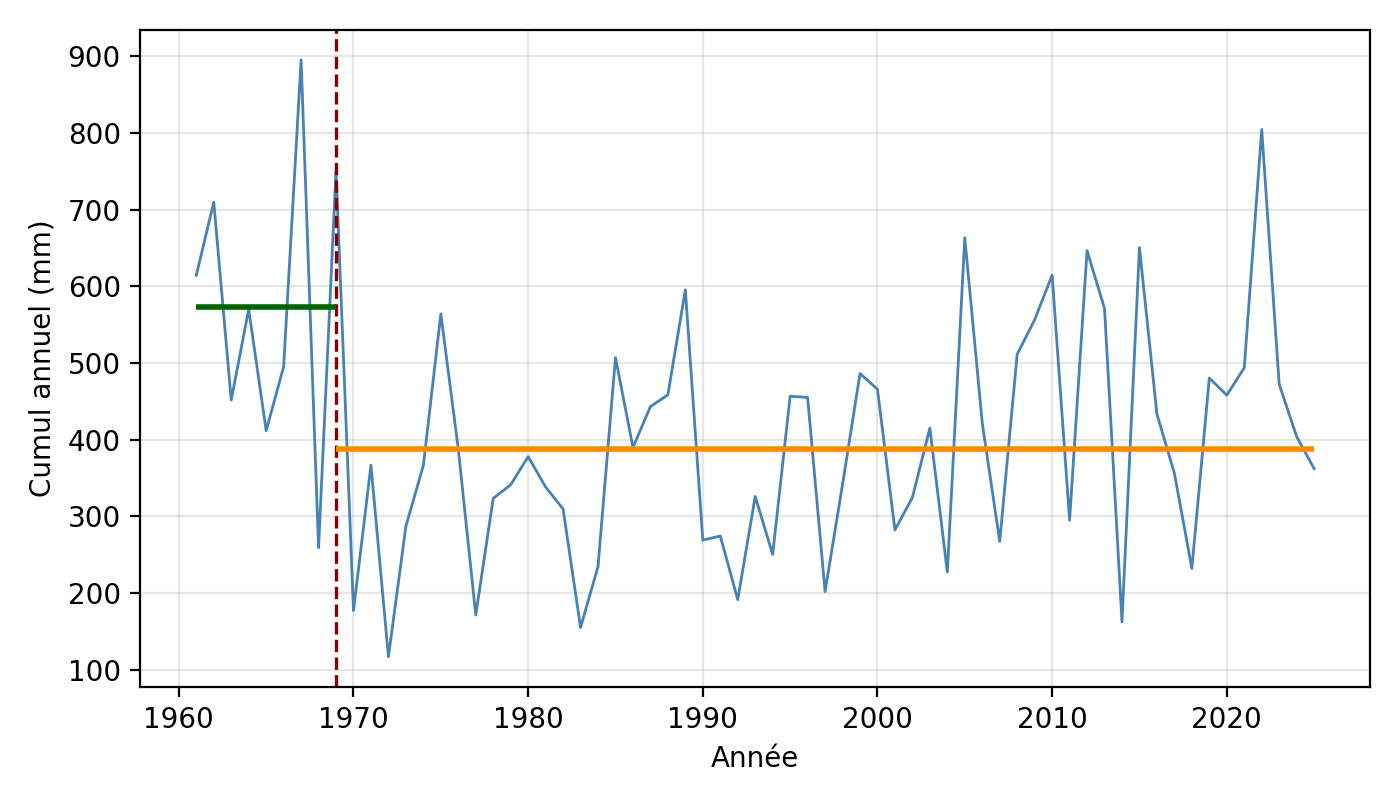
\includegraphics[width=0.70\linewidth]{prism-uploads/Dakar_2.png}};
  % Bordures noires renforcées sur le cadre des axes, sans modifier les données.
  \begin{scope}[x={(dakargraph.south east)},y={(dakargraph.north west)}]
    \draw[black,line width=0.6pt] (0.1004,0.1404) rectangle (0.9786,0.9638);
  \end{scope}
\end{tikzpicture}
\smallskip
\begin{minipage}{\linewidth}
\footnotesize
\textit{Lecture :} La courbe bleue représente le cumul annuel ; les segments vert et orange indiquent les moyennes avant et après rupture. Le trait rouge discontinu repère l'année de rupture.
\end{minipage}
\par\smallskip
\begin{center}
{\small\itshape Source : ANACIM, calculs de l’auteur.}
\end{center}
\end{figure}

Un second groupe de deux régions, que sont Fatick et Ziguinchor, présente à l'inverse une rupture plus récente, en 2007, marquée par une hausse du cumul pluviométrique régional après une longue phase stable (figure~\ref{fig:rupture-fatick}, région de Fatick). Ce résultat est cohérent avec la reprise pluviométrique partielle observée au Sahel depuis le début des années 2000, parfois désignée sous le terme de « reverdissement du Sahel ».

\begin{figure}[H]
\centering
\caption{Évolution du cumul pluviométrique régional annuel à Fatick et rupture détectée en 2007}
\label{fig:rupture-fatick}
\begin{tikzpicture}
  \node[anchor=south west,inner sep=0pt] (fatickgraph) at (0,0)
    {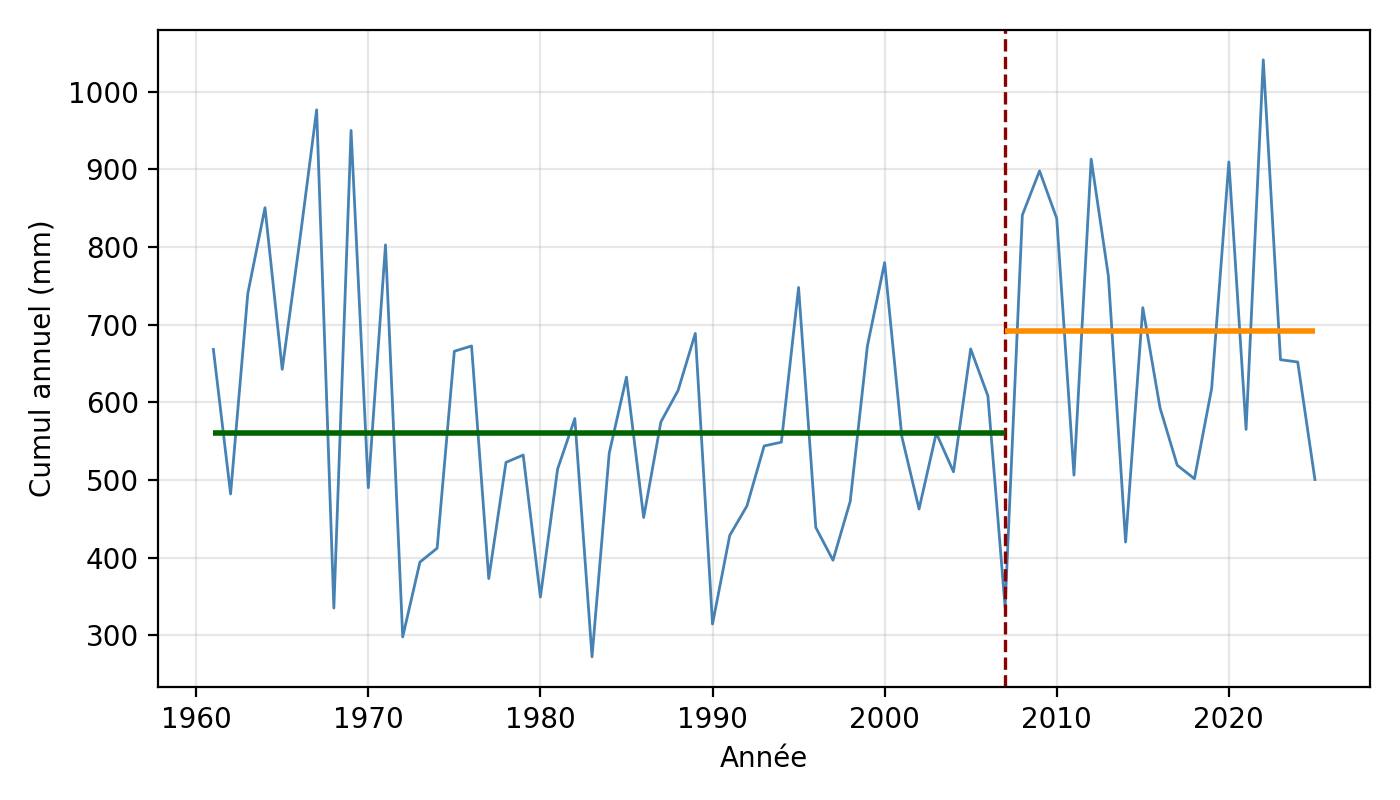
\includegraphics[width=0.70\linewidth]{prism-uploads/Fatick_3.png}};
  % Même épaisseur de bordure que le graphique de Dakar.
  \begin{scope}[x={(fatickgraph.south east)},y={(fatickgraph.north west)}]
    \draw[black,line width=0.6pt] (0.1136,0.1404) rectangle (0.9786,0.9638);
  \end{scope}
\end{tikzpicture}
\smallskip
\begin{minipage}{\linewidth}
\footnotesize
\textit{Lecture :} La courbe bleue représente le cumul annuel ; les segments vert et orange indiquent les moyennes avant et après rupture. Le trait rouge discontinu repère l'année de rupture.
\end{minipage}
\par\smallskip
\begin{center}
{\small\itshape Source : ANACIM, calculs de l’auteur.}
\end{center}
\end{figure}

Kaffrine constitue un cas isolé, avec une rupture détectée en 1998, également marquée par une hausse du cumul pluviométrique régional, mais sans qu'un regroupement avec d'autres régions ne soit observé sur cette date précise.

\subsubsection*{Régions sans rupture avérée}

Les six régions restantes que sont Kaolack, Kolda, Louga, Matam, Tambacounda et Thiès ne satisfont pas au critère de majorité (2 tests convergents sur 4 seulement) et sont donc considérées comme ne présentant pas de rupture avérée sur la période 1961-2025. Ce résultat mérite d'être nuancé pour deux d'entre elles : à Kaolack et à Matam, la non-validation de la rupture est cohérente avec les anomalies identifiées lors du diagnostic préalable (tendance progressive pour la première, autocorrélation pour la seconde). Ces anomalies tendent à produire de fausses significativités chez certains tests pris isolément (\textsc{Pettitt} et \textsc{Buishand} dans les deux cas), sans qu’il soit possible de conclure à une véritable discontinuité dans la série. Pour Louga et Tambacounda, aucune anomalie méthodologique préalable n’a été détectée. L’absence de rupture avérée traduit un signal de discontinuité trop faible ou trop diffus pour atteindre le seuil de robustesse retenu. Kolda et Thiès, enfin, constituent des cas limites car l’analyse de sensibilité (\hyperref[tab:sensibilite-tolerance-ruptures]{annexe~F}) montre qu’elles deviennent avérées pour une tolérance de ±4 ans, alors que les quatre autres régions restent non avérées jusqu’à ±5 ans. Leur non-validation dépend donc du choix de la tolérance et doit être interprétée avec prudence.

L'ensemble des 14 séries pluviométriques régionales annotées, incluant les six régions sans rupture avérée, est présenté en \hyperref[ann:series-ruptures]{annexe~A} (figure~\ref{fig:series-ruptures-annexe}).

\subsection{Résultats de la comparaison des moyennes avant et après rupture}

Afin de quantifier l'ampleur du changement associé à chaque rupture détectée, une comparaison statistique des moyennes pluviométriques avant et après la date de rupture retenue (date majoritaire) a été effectuée pour les huit régions présentant une rupture avérée. L'homoscédasticité des deux sous-périodes a été vérifiée au préalable par un test de Levene ; le test de Student a été appliqué lorsque les variances étaient homogènes, et le test de Welch dans le cas contraire. Les résultats sont présentés dans le tableau suivant.


\begin{table}[H]
\centering
\caption[Comparaison des moyennes pluviométriques avant et après rupture pour les huit régions présentant une rupture avérée]{Comparaison des moyennes pluviométriques avant et après rupture pour les huit régions présentant une rupture avérée\protect\footnotemark}
\label{tab:comparaison-moyennes-rupture}
\begingroup
\fontsize{8.5}{10.5}\selectfont
\setlength{\tabcolsep}{2pt}
\renewcommand{\arraystretch}{1.45}
\begin{tabular*}{\linewidth}{@{\extracolsep{\fill}}lrrrrrrclrrc@{}}
\toprule
\rowcolor{navyblue}
\textcolor{white}{\textbf{Région}} &
\textcolor{white}{\shortstack{\textbf{Année de}\\\textbf{rupture}}} &
\textcolor{white}{\shortstack{$\boldsymbol{n}$\\\textbf{avant}}} &
\textcolor{white}{\shortstack{$\boldsymbol{n}$\\\textbf{après}}} &
\textcolor{white}{\shortstack{\textbf{Moyenne}\\\textbf{avant}\\\textbf{(mm)}}} &
\textcolor{white}{\shortstack{\textbf{Moyenne}\\\textbf{après}\\\textbf{(mm)}}} &
\textcolor{white}{\shortstack{\textbf{Variation}\\\textbf{(\%)}}} &
\textcolor{white}{\shortstack{\textbf{Variances}\\\textbf{égales}}} &
\textcolor{white}{\shortstack{\textbf{Test}\\\textbf{utilisé}}} &
\multicolumn{1}{c}{\textcolor{white}{$\boldsymbol{t}$}} &
\textcolor{white}{\shortstack{\textbf{Valeur}\\$\boldsymbol{p}$}} &
\textcolor{white}{\shortstack{\textbf{Signif.}\\\textbf{à 5\%}}} \\
\midrule
\rowcolor{navyblue!7}
\textbf{Dakar}       & 1969 &  9 & 56 & 573,11  & 388,09  & $-32{,}30$ & Oui & Student & $3{,}33$  & $<0{,}01$ & Oui \\
\textbf{Kédougou}    & 1966 &  6 & 59 & 1\,400,30 & 1\,174,14 & $-16{,}20$ & Non & Welch   & $7{,}45$  & $<0{,}01$ & Oui \\
\rowcolor{navyblue!7}
\textbf{Saint-Louis} & 1969 &  9 & 56 & 360,49  & 257,15  & $-28{,}70$ & Oui & Student & $2{,}90$  & $<0{,}01$ & Oui \\
\textbf{Diourbel}    & 1971 & 11 & 54 & 644,39  & 508,47  & $-21{,}10$ & Oui & Student & $3{,}09$  & $<0{,}01$ & Oui \\
\rowcolor{navyblue!7}
\textbf{Fatick}      & 2007 & 47 & 18 & 560,50  & 691,92  & 23,40     & Oui & Student & $-2{,}77$ & $<0{,}01$ & Oui \\
\textbf{Sédhiou}     & 1969 &  9 & 56 & 1\,414,31 & 1\,085,85 & $-23{,}20$ & Oui & Student & $3{,}62$  & $<0{,}01$ & Oui \\
\rowcolor{navyblue!7}
\textbf{Ziguinchor}  & 2007 & 47 & 18 & 1\,280,49 & 1\,496,61 & 16,90     & Oui & Student & $-2{,}68$ & $<0{,}01$ & Oui \\
\textbf{Kaffrine}    & 1998 & 38 & 27 & 587,51  & 710,72  & 21,00     & Oui & Student & $-3{,}39$ & $<0{,}01$ & Oui \\
\bottomrule
\end{tabular*}
\endgroup
\tablesource
\end{table}
\footnotetext{$n$ désigne le nombre d'observations de chaque sous-période. L'égalité des variances est évaluée par le test de Levene. La dernière colonne indique si la différence de moyennes est significative au seuil de 5\%. Pour Kédougou, $p<0{,}001$. L'année de rupture est comptée dans la période « avant ».}

L'analyse du tableau ci-dessus confirme et quantifie les deux groupes de ruptures. Les cinq régions de Kédougou, Dakar, Saint-Louis, Sédhiou et Diourbel, dont la rupture se situe entre 1966 et 1971, présentent toutes une baisse de la moyenne pluviométrique annuelle après rupture. Ce déficit oscille entre $-16{,}2$\% pour Kédougou et $-32{,}3$\% pour Dakar. Une telle baisse, de l'ordre d'un sixième à un tiers du cumul régional moyen, illustre la sévérité du déficit associé à l'installation de la sécheresse sahélienne sur la période. À l'inverse, les trois régions dont la rupture est plus récente (à savoir Kaffrine en 1998, puis Fatick et Ziguinchor en 2007) présentent toutes une hausse significative. Cette augmentation, comprise entre $+16{,}9$\% et $+23{,}4$\%, est cohérente avec la phase de reprise pluviométrique partielle observée au Sahel depuis la fin des années 1990.

Un résultat mérite d'être nuancé : à Kédougou, le test de Levene a révélé une hétérogénéité des variances entre les deux sous-périodes, conduisant à l'utilisation du test de Welch plutôt que du test de Student classique. Cette adaptation méthodologique n'affecte pas la conclusion, la différence restant hautement significative ($p<0{,}001$), mais illustre l'intérêt d'une vérification systématique de l'homoscédasticité avant toute comparaison de moyennes.

\clearpage
\section{Analyse en Composantes Principales (ACP)}

\subsection{Résultats de l'Analyse en composantes principales}

La mise en œuvre de l'ACP a consisté à définir au préalable un tableau de données croisant les 65 années d'observation (1961-2025) et les 14 séries pluviométriques régionales centrées-réduites, puis à calculer la matrice de corrélation entre ces séries. Cette matrice a ensuite fait l'objet d'une diagonalisation, opération qui a permis d'extraire les valeurs propres et les vecteurs propres associés à chaque axe factoriel. Les valeurs propres obtenues sont consignées dans le tableau ci-dessous. Elles renseignent la part de la variance totale captée par chaque axe. Le nombre d'axes retenus pour l'interprétation a été fixé selon le critère de Kaiser, qui ne conserve que les axes dont la valeur propre excède 1.

\begin{table}[H]
\centering
\captionsetup{justification=centering,skip=2pt}
\caption{Valeurs propres, variance expliquée et sélection des axes selon le critère de Kaiser}
\label{tab:valeurs-propres-acp}
\begingroup
\footnotesize
\setlength{\tabcolsep}{7pt}
\renewcommand{\arraystretch}{1.0}
\begin{tabularx}{0.90\textwidth}{@{}l*{4}{>{\centering\arraybackslash}X}@{}}
\toprule
\rowcolor{navyblue}
\textcolor{white}{\textbf{Axe}} &
\textcolor{white}{\textbf{Valeur propre}} &
\textcolor{white}{\shortstack{\textbf{Variance}\\\textbf{expliquée (\%)}}} &
\textcolor{white}{\shortstack{\textbf{Variance}\\\textbf{cumulée (\%)}}} &
\textcolor{white}{\textbf{Oui/Non}} \\
\midrule
\rowcolor{navyblue!7}
\textbf{Axe 1}  & 7,76 & 54,59 & 54,59  & Oui \\
\textbf{Axe 2}  & 1,20 & 8,41  & 63,00  & Oui \\
\rowcolor{navyblue!7}
\textbf{Axe 3}  & 0,93 & 6,51  & 69,51  & Non \\
\textbf{Axe 4}  & 0,68 & 4,78  & 74,29  & Non \\
\rowcolor{navyblue!7}
\textbf{Axe 5}  & 0,64 & 4,47  & 78,76  & Non \\
\textbf{Axe 6}  & 0,52 & 3,63  & 82,39  & Non \\
\rowcolor{navyblue!7}
\textbf{Axe 7}  & 0,46 & 3,20  & 85,59  & Non \\
\textbf{Axe 8}  & 0,43 & 3,04  & 88,63  & Non \\
\rowcolor{navyblue!7}
\textbf{Axe 9}  & 0,38 & 2,65  & 91,27  & Non \\
\textbf{Axe 10} & 0,31 & 2,21  & 93,48  & Non \\
\rowcolor{navyblue!7}
\textbf{Axe 11} & 0,30 & 2,12  & 95,61  & Non \\
\textbf{Axe 12} & 0,27 & 1,92  & 97,53  & Non \\
\rowcolor{navyblue!7}
\textbf{Axe 13} & 0,20 & 1,41  & 98,94  & Non \\
\textbf{Axe 14} & 0,15 & 1,06  & 100,00 & Non \\
\bottomrule
\end{tabularx}
\endgroup
\tablesource
\end{table}

Deux axes seulement présentent une valeur propre supérieure à 1. Ils sont donc retenus pour l'interprétation. Ensemble, ils expliquent 62,99\% de la variance totale. L'Axe 1 concentre à lui seul plus de la moitié de l'information (54,59\%).

\begin{figure}[H]
\centering
\captionsetup{justification=centering,skip=3pt}
\caption{Éboulis des valeurs propres de l'ACP et seuil de Kaiser}
\label{fig:eboulis-valeurs-propres-acp}
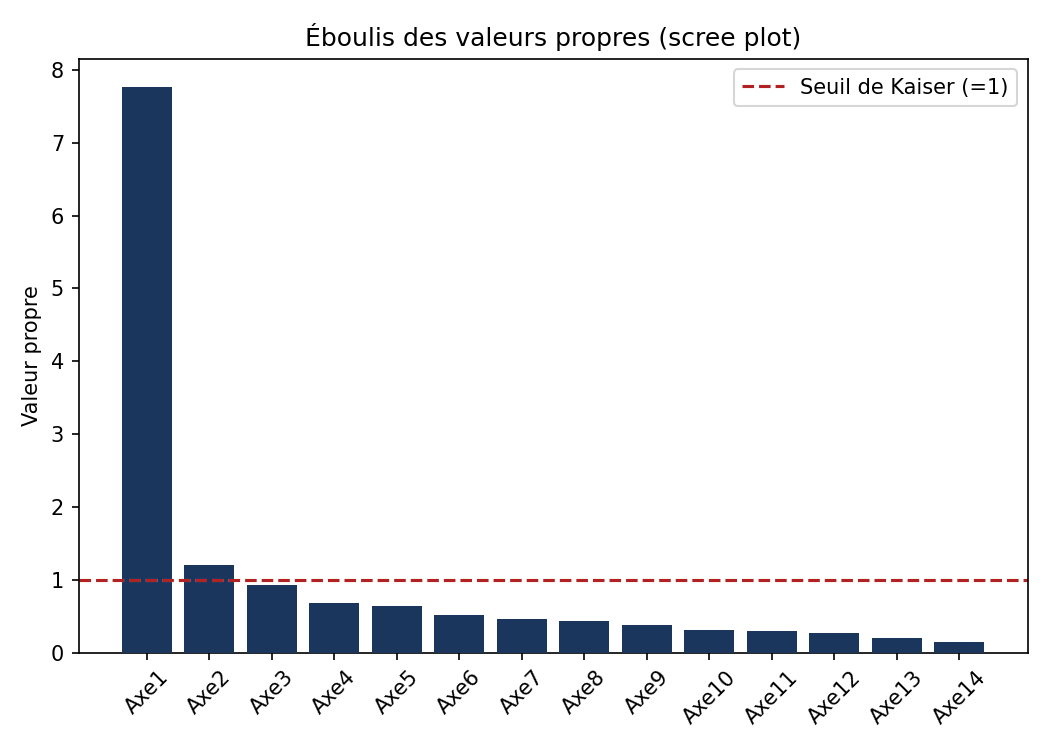
\includegraphics[width=0.48\linewidth,keepaspectratio]{prism-uploads/graph4_eboulis_acp_bleu_fonce.png}
\par\smallskip
{\small\itshape Source : ANACIM, calculs de l’auteur.}\par
\end{figure}

L’éboulis ne permet pas de trancher de façon univoque. La chute nette d’inertie entre l’Axe 1 et l’Axe 2, suivie d’une décroissance progressive, suggérerait de ne retenir que le premier axe d’après la \textbf{Règle du coude de Cattell}\footnote{Règle du coude de Cattell : C'est une méthode graphique de choix du nombre d’axes d’une analyse factorielle. On observe l’éboulis des valeurs propres et on retient les axes situés avant le point où la courbe cesse de chuter fortement et devient presque plate.}. Le critère de Kaiser, retenu ici, conserve deux axes, l’Axe 2 se situant toutefois à peine au-dessus du seuil ($\lambda = 1{,}20$). Ce second axe est conservé parce qu’il porte une information interprétable et qu’il permet de représenter les années dans le plan factoriel. Son interprétation est donc présentée avec prudence.

La contribution de chaque région aux deux axes retenus est représentée par le cercle des corrélations.

\begin{figure}[H]
\centering
\captionsetup{justification=centering,skip=4pt}
\caption{Cercle des corrélations des variables pluviométriques régionales sur les deux premiers axes de l'ACP}
\label{fig:cercle-correlations-acp}
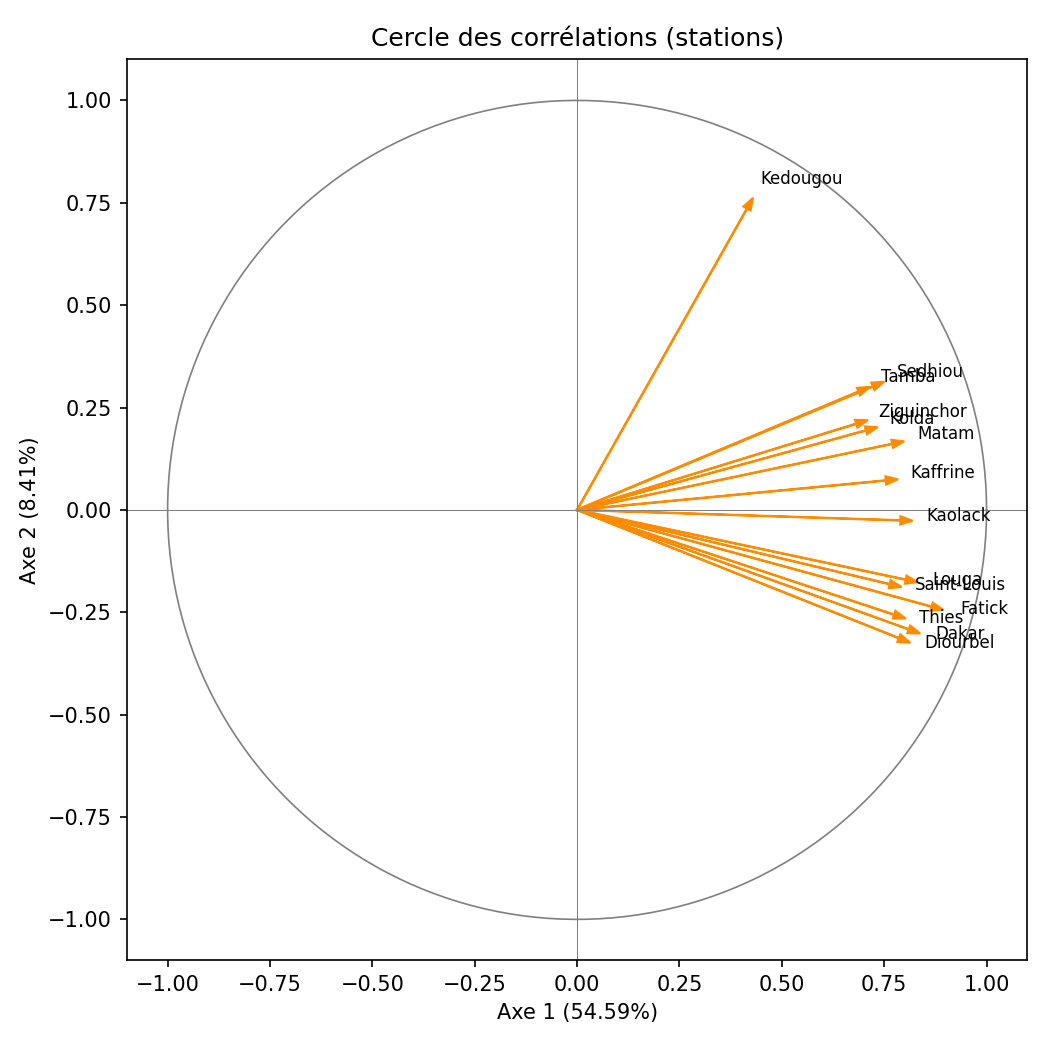
\includegraphics[width=0.58\linewidth,trim=0 0 0 25bp,clip,keepaspectratio]{prism-uploads/graph5_cercle_correlations.png}
\smallskip
\begin{minipage}{0.96\linewidth}
\small
\begin{justify}
Toutes les régions présentent une corrélation positive avec l'Axe 1. Elle varie de $0{,}41$ pour Kédougou à $0{,}87$ pour Fatick. La majorité des régions dépasse $0{,}70$. Sur l’Axe 2, les corrélations sont plus contrastées. Certaines régions sont positivement corrélées (Kédougou : $0{,}74$ ; Sédhiou : $0{,}30$ ; Tambacounda : $0{,}29$ ; Ziguinchor : $0{,}21$ ; Kolda : $0{,}19$ ; Matam : $0{,}16$). D’autres le sont négativement (Diourbel : $-0{,}31$ ; Dakar : $-0{,}29$ ; Thiès : $-0{,}26$ ; Fatick : $-0{,}24$ ; Saint-Louis : $-0{,}18$ ; Louga : $-0{,}17$). Kaffrine ($0{,}07$) et Kaolack ($-0{,}03$) sont proches de zéro.
\end{justify}
\end{minipage}
\par\smallskip
\begin{center}
{\small\itshape Source : ANACIM, calculs de l’auteur.}
\end{center}
\end{figure}





\subsection{Interprétation des axes retenus}
\label{sec:interpretation-axes}

L'Axe 1 regroupe toutes les régions avec un signe positif. Il traduit un signal pluviométrique commun à l'ensemble du territoire. Une année où l'Axe 1 est élevé correspond ainsi à une année globalement excédentaire à l'échelle nationale. Inversement, une valeur faible traduit une année globalement déficitaire. Ce résultat est cohérent avec la forte part de variance qu'il explique : la variabilité pluviométrique au Sénégal est avant tout un phénomène national, avant d'être un phénomène propre à chaque région.

L’Axe 2 traduit un contraste géographique secondaire, par rapport au signal national porté par l’Axe 1. Il oppose les régions de l’Est et du Sud (Kédougou, Sédhiou, Tambacounda, Ziguinchor, Kolda, Matam) à celles de la façade occidentale, du Nord-Ouest au Centre-Ouest (Dakar, Diourbel, Thiès, Fatick, Saint-Louis, Louga). Ce contraste n’est pas strictement latitudinal : Matam, au nord-est, se place du côté positif. À l’exception de Kédougou (0,74), toutes les corrélations restent inférieures à 0,32 en valeur absolue.

La région de Kédougou se distingue des autres. Sa corrélation avec l’Axe 1 est la plus faible ($0{,}41$), tandis que sa corrélation avec l’Axe 2 est la plus forte ($0{,}74$). Cette position particulière dans l’espace factoriel traduit un comportement pluviométrique distinct de celui des autres régions. Elle peut être mise en relation avec sa position méridionale et son appartenance au domaine soudano-guinéen.

Ces deux axes offrent donc une lecture complémentaire de la variabilité pluviométrique sénégalaise : une dynamique nationale dominante (Axe 1), doublée d’un contraste entre le Sud-Est et l’Ouest, plus secondaire (Axe 2).


L'analyse en composantes principales met ainsi en évidence deux dimensions complémentaires de la variabilité pluviométrique au Sénégal. L'Axe 1, largement dominant, traduit un signal pluviométrique commun à l'ensemble du territoire national. L'Axe 2, plus secondaire, révèle un contraste géographique opposant l’Est et le Sud à l’Ouest. Cette structuration en deux composantes prépare la classification des années selon les régimes pluviométriques, présentée dans la section suivante.

\enlargethispage{1cm}
\section{Classification des années selon les régimes pluviométriques}
\label{sec:classification-annees}

\subsection{Typologie des régimes pluviométriques obtenus}
\label{sec:typologie-regimes}

La classification a été appliquée aux coordonnées factorielles des deux axes retenus par le critère de Kaiser. Une classification ascendante hiérarchique (CAH) a été réalisée, selon le critère de Ward et la distance euclidienne. Le dendrogramme obtenu retrace les regroupements successifs des 65 années d'observation (voir \hyperref[fig:dendrogramme-classification-annees]{annexe~E}, figure~\ref{fig:dendrogramme-classification-annees}).

Le nombre de classes a été fixé à trois, conformément à la typologie recherchée, à savoir les années sèches, normales et humides. L’examen du dendrogramme (\hyperref[fig:dendrogramme-classification-annees]{annexe~E}, figure~\ref{fig:dendrogramme-classification-annees}) montre toutefois que le saut d’inertie le plus marqué correspond à une partition en deux classes. En effet, la première bifurcation isole un groupe homogène d’années humides, tandis que la seconde ne sépare pas nettement les années normales des années sèches. Le choix de trois classes relève donc d’un critère d’interprétation et non d’un critère statistique.

Le tableau suivant présente la moyenne pluviométrique nationale de chaque classe.

\begin{table}[H]
\centering
\captionsetup{justification=centering}
\caption{Caractéristiques pluviométriques des trois classes d'années}
\label{tab:classes-regimes-pluviometriques}
\begingroup
\small
\setlength{\tabcolsep}{3pt}
\renewcommand{\arraystretch}{1.2}
\begin{tabularx}{0.82\textwidth}{@{}c*{4}{>{\centering\arraybackslash}X}l@{}}
\toprule
\rowcolor{navyblue}
\textcolor{white}{\textbf{Classe}} &
\textcolor{white}{\textbf{Moyenne (mm)}} &
\textcolor{white}{\textbf{Min. (mm)}} &
\textcolor{white}{\textbf{Max. (mm)}} &
\textcolor{white}{\textbf{Nombre d'années}} &
\textcolor{white}{\textbf{Régime}} \\
\midrule
1 & 823,20 & 717,70 & 977,80 & 25 & Humide \\
\rowcolor{navyblue!7}
2 & 714,30 & 635,70 & 799,20 & 10 & Normal \\
3 & 584,90 & 418,20 & 692,20 & 30 & Sec \\
\bottomrule
\end{tabularx}
\endgroup
\tablesource
\end{table}

Les plages de cumul de deux classes voisines se recouvrent partiellement, car la classification repose sur les coordonnées factorielles et non sur le cumul national seul.

Trois régimes pluviométriques distincts se dégagent ainsi. Le régime sec regroupe
le plus grand nombre d’années (30 sur 65), suivi du régime humide (25 années). Le
régime normal, plus restreint, ne compte que 10 années.

\subsection{Interprétation des résultats de classification}

La projection des années sur le plan factoriel, colorée selon leur régime, permet de visualiser la cohérence de cette classification avec la structure mise en évidence par l'ACP.

\begin{figure}[H]
\centering
\captionsetup{justification=centering}
\caption{Projection des années sur les deux premiers axes de l'ACP selon leur régime pluviométrique}
\label{fig:projection-annees-regimes}
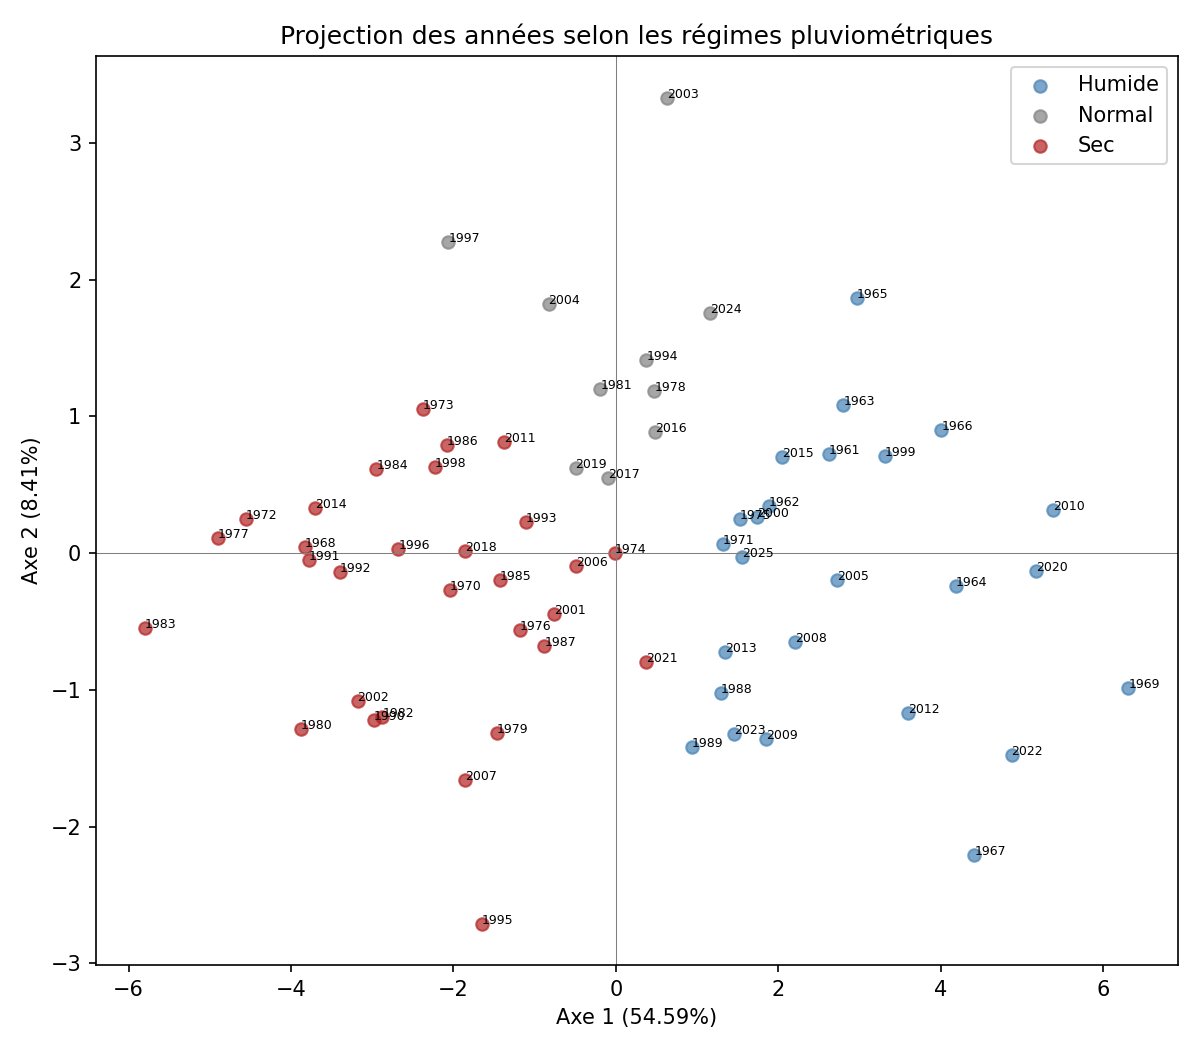
\includegraphics[width=0.72\linewidth,keepaspectratio]{prism-uploads/graph6_projection_annees.png}
\par\smallskip
\begin{center}
{\small\itshape Source : ANACIM, calculs de l’auteur.}
\end{center}
\end{figure}

Les années humides se positionnent majoritairement à droite du plan, du côté positif de l'Axe 1. Les années sèches se positionnent à l'inverse du côté négatif. Les années normales se concentrent quant à elles autour de l’origine de l’Axe 1, avec des valeurs majoritairement positives sur l’Axe 2. La classification en trois régimes repose donc surtout sur l’Axe 1, ce qui est cohérent avec son interprétation comme signal pluviométrique national.

Le régime normal apparaît ainsi moins comme un troisième pôle distinct que comme une zone de transition entre les deux régimes extrêmes. Le dendrogramme confirme cette lecture : la première bifurcation, la plus haute en inertie, sépare nettement les années humides du reste de la série. La seconde bifurcation, en revanche, n'isole pas clairement les années normales des années sèches, ces dernières se répartissant entre les deux sous-groupes formés à ce niveau.

L'examen chronologique des classes fait par ailleurs apparaître une cohérence avec les ruptures identifiées en \hyperref[sec:analyse-ruptures]{IV.2}. Les années 1961 à 1967 sont quasi exclusivement classées en régime humide. La période 1968-1987 bascule massivement en régime sec, à quelques exceptions près. Depuis 2008, une recrudescence du régime humide est observée. Cette évolution correspond aux deux groupes de ruptures précédemment mis en évidence, le premier autour de 1966-1971, le second autour de 2007.


La classification des années confirme ainsi l'existence de régimes pluviométriques distincts au Sénégal, structurés pour l'essentiel par le signal national porté par l'Axe 1 de l'ACP. Elle met également en évidence une cohérence temporelle forte avec les ruptures détectées dans les séries chronologiques, deux approches méthodologiques indépendantes convergeant ainsi vers une même lecture de la dynamique pluviométrique nationale.

\subsection{Illustration régionale des régimes pluviométriques}
\label{sec:illustration-regionale}

Si la classification obtenue en \hyperref[sec:typologie-regimes]{IV.4.1} repose sur les coordonnées factorielles synthétiques issues de l’ACP, il est utile d’en vérifier la cohérence au niveau de chacune des quatorze régions prises individuellement. Les figures~\ref{fig:ips-lisse-dakar} et \ref{fig:ips-lisse-kedougou} présentent l’indice pluviométrique standardisé de Dakar et de Kédougou, lissé à l’aide du filtre passe-bas de Hanning d’ordre 2. Ce lissage atténue les fluctuations d’une année à l’autre afin de mieux faire apparaître les phases pluriannuelles, humides ou sèches.

\subsubsection*{Dakar : une région représentative du signal national}

\begin{figure}[H]
\centering
\captionsetup{justification=centering}
\caption{Indice pluviométrique standardisé lissé, région de Dakar (1961-2025)}
\label{fig:ips-lisse-dakar}
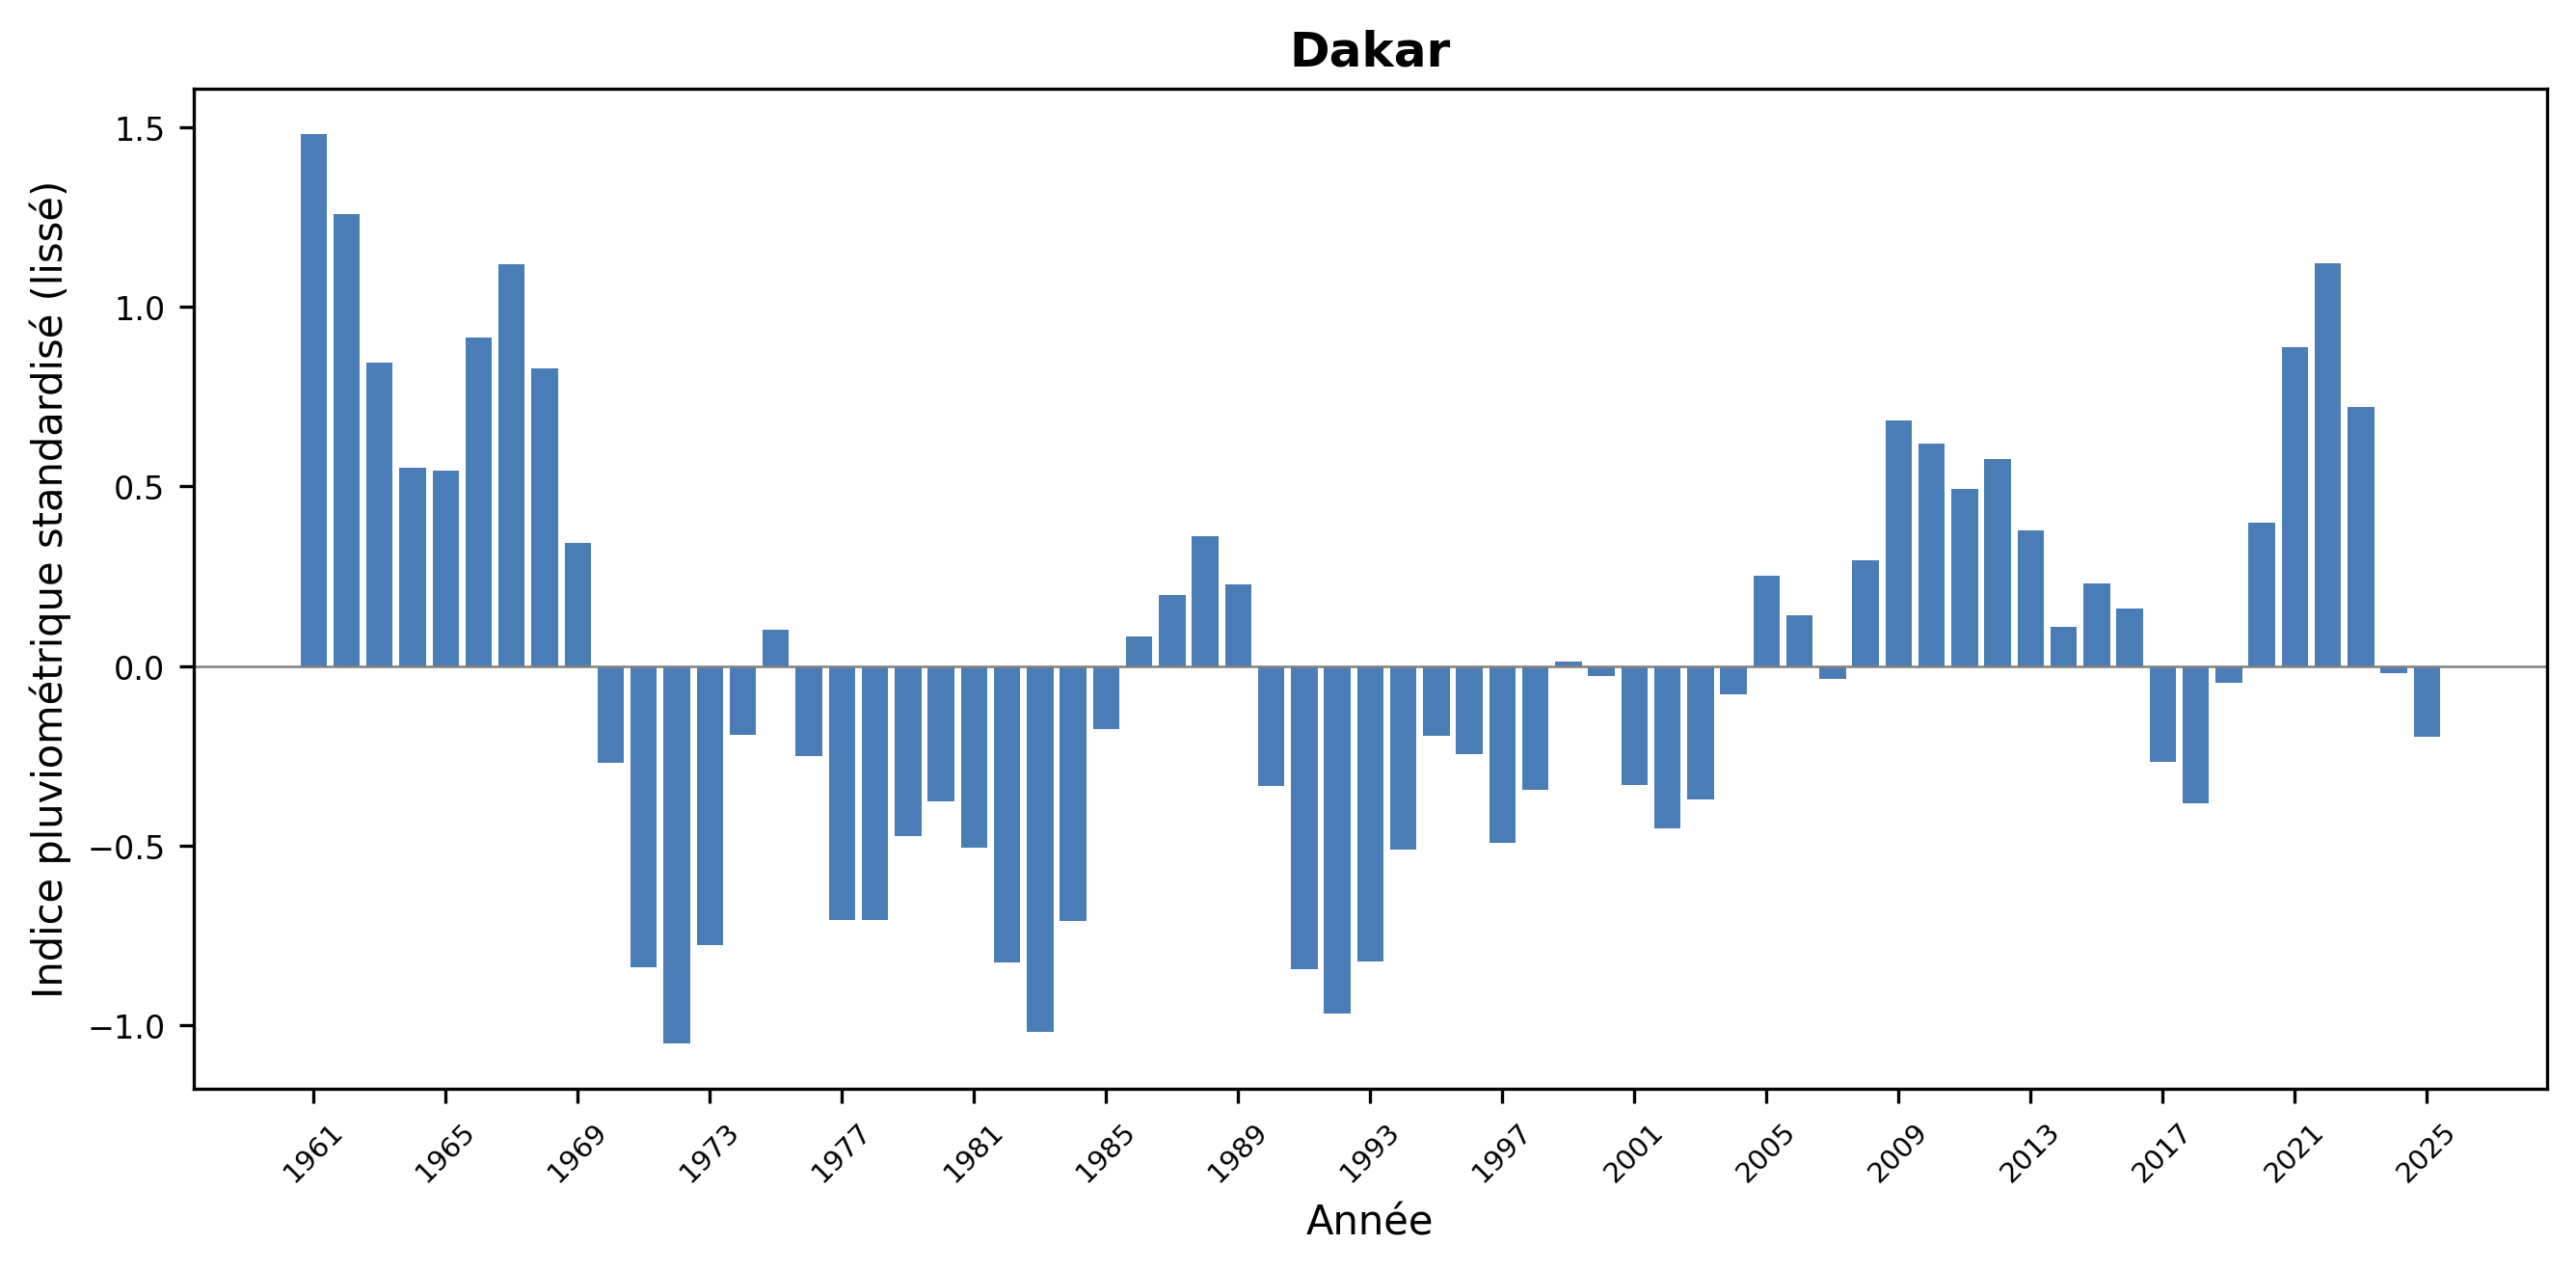
\includegraphics[width=0.84\linewidth,height=0.38\textheight,keepaspectratio]{prism-uploads/Figure_IV4_3_Dakar.png}
\par\smallskip
\begin{center}
{\small\itshape Source : ANACIM, calculs de l’auteur.}
\end{center}
\end{figure}

La série de Dakar reproduit fidèlement la structuration en trois phases déjà identifiée à l'échelle nationale. Une phase humide s'étend de 1961 à 1968, avec un maximum proche de $+1{,}5$ en 1961, suivie d'un basculement net dès 1969. Cette date est cohérente avec la rupture détectée par trois des quatre tests statistiques (\hyperref[sec:resultats-detection-ruptures]{IV.2.1}). La phase déficitaire se prolonge jusqu'au milieu des années 2000, avec deux creux marqués vers 1972-1973 et 1983-1984, proches de $-1{,}1$, séparés par une brève rémission entre 1988 et 1992. La reprise s'amorce à partir de 2005-2006, avec deux pics autour de 2009-2011 et 2020-2021 ($+0{,}7$ à $+1{,}1$), avant un retour à des valeurs proches de zéro en fin de série. Cette lecture confirme la pertinence de l'indice national (figure~\ref{fig:evolution-temporelle-indice-moyen}) comme reflet de la dynamique dakaroise.

\subsubsection*{Kédougou : une trajectoire décalée par rapport au signal national}

\begin{figure}[H]
\centering
\captionsetup{justification=centering}
\caption{Indice pluviométrique standardisé lissé, région de Kédougou (1961-2025)}
\label{fig:ips-lisse-kedougou}
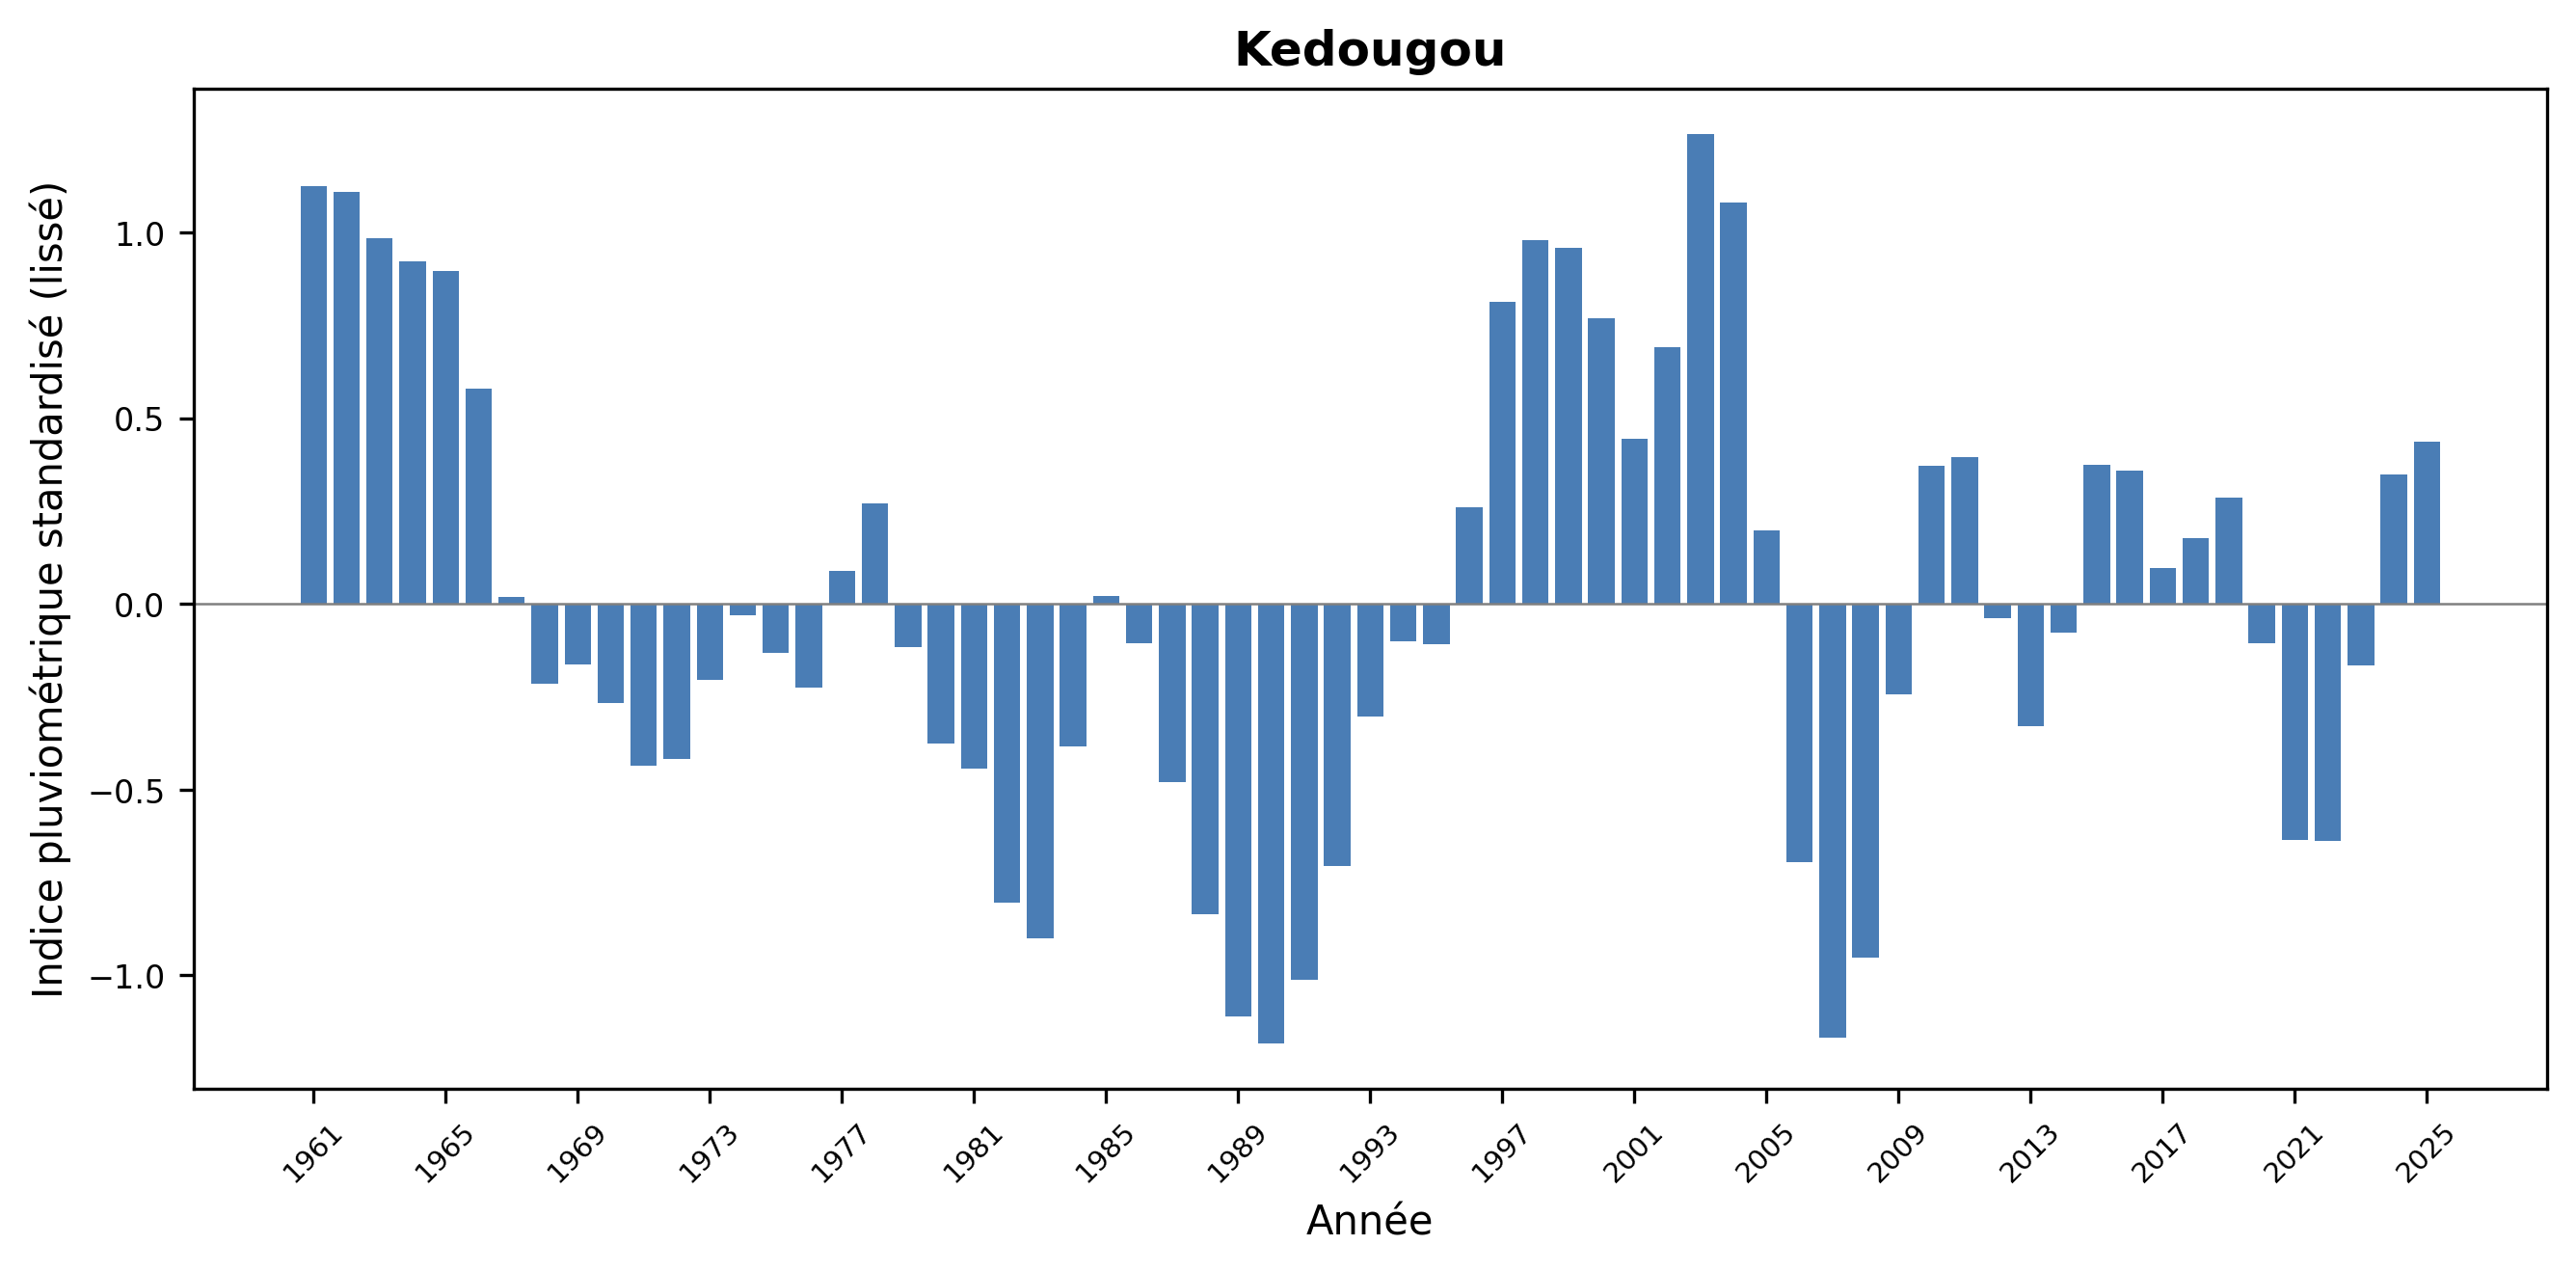
\includegraphics[width=0.84\linewidth,height=0.38\textheight,keepaspectratio]{prism-uploads/Figure_IV4_3_Kedougou.png}
\par\smallskip
\begin{center}
{\small\itshape Source : ANACIM, calculs de l’auteur.}
\end{center}
\end{figure}

La série de Kédougou illustre le comportement singulier déjà relevé en \hyperref[sec:interpretation-axes]{IV.3.2}, où cette région présentait la corrélation la plus faible avec l'Axe 1 ($0{,}41$) et la plus forte avec l'Axe 2 ($0{,}74$). La phase humide initiale et la rupture de 1966 se retrouvent bien, en cohérence avec le reste du territoire. La suite s'en écarte cependant : après un creux limité entre 1969 et 1976, la région traverse une phase excédentaire prononcée entre 1991 et 2004, avec des pics dépassant $+1{,}2$, alors que Dakar demeure encore en plein déficit sur cette période. Ce n'est qu'à partir de 2006-2007 que Kédougou rejoint une dynamique déficitaire brève, avant une reprise plus modérée et heurtée, sans retrouver l'amplitude de ses pics antérieurs à 1969. Cette avance d'une dizaine d'années dans la reprise pluviométrique illustre concrètement la singularité du Sud-Est, portée par l’Axe 2 : la dynamique du Sud-Est, sous influence soudano-guinéenne, ne suit pas strictement le calendrier de la sécheresse sahélienne.

\subsubsection*{Lecture d'ensemble des quatorze régions (\hyperref[fig:ips-lisses-regions-annexe]{annexe B})}

L'examen des autres séries régionales confirme que le profil de Dakar est largement majoritaire : Saint-Louis, Diourbel, Fatick, Kolda, Louga, Sédhiou, Matam, Tambacounda, Thiès et Ziguinchor présentent tous une phase humide initiale, un creux prolongé entre 1970 et 1990, et une reprise nette depuis le milieu des années 2000, avec une intensité variable selon les régions. Le déficit est particulièrement marqué à Diourbel et Tambacounda, où les minima sont proches respectivement de $-1{,}4$ et $-1{,}3$. Kaolack se distingue par une reprise récente atteignant des valeurs élevées en fin de série, proches de $+2{,}0$. Kédougou demeure la seule région à présenter un décrochage temporel aussi marqué par rapport au calendrier national. Kaffrine présente un profil différent. Véritablement sans une phase humide initiale marquée, elle connaît un creux plus tardif, au tournant des années 1980-1990, puis une reprise nette autour de 1998, en cohérence avec la rupture détectée à cette date.

Cette lecture région par région permet une vérification qualitative de la cohérence entre dynamique nationale et dynamiques locales ; elle ne constitue pas un nouveau test statistique, mais un appui visuel à l'interprétation de la CAH. Elle conforte la lecture de l’Axe 2 comme contraste structurant une variabilité régionale additionnelle au signal national porté par l’Axe 1, et illustre concrètement la position atypique de Kédougou déjà identifiée par les coefficients de corrélation factoriels.

\section{Discussion}

L’analyse des quatorze séries pluviométriques met en évidence deux périodes de changement, à la fin des années 1960 puis autour des années 2000, ainsi qu’un contraste régional secondaire révélé par l’ACP. Ces résultats permettent de revenir sur les hypothèses formulées en introduction.

L’hypothèse H1, relative à l’existence d’une rupture statistiquement significative, peut être confirmée. En effet, huit (08) régions sur quatorze (14) présentent une rupture avérée, fondée sur la convergence d’au moins trois des quatre procédures utilisées.

L'hypothèse H2 est confirmée : la différence entre les moyennes avant et après rupture est significative au seuil de 5\% dans les huit régions concernées.

L’hypothèse H3 est confirmée de façon nuancée par l’ACP, qui reste une méthode descriptive et exploratoire. En effet, le second axe, qui n’explique que 8,4\% de la variance, oppose globalement l’Est et le Sud à l’Ouest, ce contraste ne coïncidant pas exactement avec un gradient Nord–Sud. Il est principalement porté par Kédougou. Cette structuration spatiale, indépendante de l’analyse des ruptures, traduit une hétérogénéité régionale du régime pluviométrique, superposée au signal national porté par le premier axe.

L’hypothèse H4 est partiellement confirmée. La CAH dégage trois classes interprétables (sèche, normale et humide) dont la répartition chronologique recoupe les deux périodes de rupture identifiées en \hyperref[sec:illustration-regionale]{IV.4.2}. La classe « normale » doit toutefois être nuancée, car le dendrogramme la présente davantage comme une zone de transition entre les deux régimes extrêmes que comme un régime pleinement distinct.

Ces résultats rejoignent plusieurs travaux antérieurs observés dans la littérature. En effet, la rupture détectée entre 1968 et 1971 dans plusieurs régions est proche de celle rapportée par Sagna et al. (2015). Ces auteurs situent la rupture sahélienne entre 1966 et 1969. Gaye (2017) aboutit aussi à des résultats similaires pour Saint-Louis, Podor et Matam. Les baisses identifiées, comprises entre 16\% et 32\%, restent du même ordre que celles rapportées par Bodian (2014), avec toutefois un maximum plus marqué à Dakar. La reprise constatée au cours des années 2000 rejoint également les résultats de Gaye (2017) et de Diop (2023).

Cette évolution peut être rapprochée des mécanismes climatiques présentés au chapitre II. Cette rupture des années 1960 peut être mise en relation avec les modifications de la mousson ouest-africaine et des conditions océaniques documentées dans la littérature. La reprise observée depuis les années 2000 traduit une amélioration partielle des conditions pluviométriques. Elle ne signifie cependant pas un retour complet au régime antérieur.

Le gradient pluviométrique Nord-Sud pourrait être dû par la position du Sénégal entre les domaines sahélien et soudano-guinéen. Les précipitations augmentent globalement vers le Sud. L’influence de la mousson y est plus importante. Cette organisation spatiale est cohérente avec les résultats de l’ACP.

Certains résultats méritent toutefois une attention particulière. Kaolack présente une tendance monotone significative. Les tests de rupture ne permettent pourtant pas de retenir une rupture selon la règle adoptée. Ce résultat montre l’intérêt de distinguer une évolution progressive d’un changement brutal. Matam constitue également un cas particulier car l’hypothèse d’indépendance y est rejetée. Cela peut contribuer à expliquer l’absence de rupture validée.

Kédougou présente aussi un comportement particulier dans l’ACP. La région se distingue des autres par sa position sur les axes factoriels. Ce résultat peut être lié à sa situation géographique et à son appartenance au domaine soudano-guinéen.

L’apport de cette étude réside ainsi dans l’analyse conjointe des quatorze régions du Sénégal sur 65 années. Elle associe l’étude des ruptures temporelles à une analyse multivariée. Cette approche permet de relier la dynamique temporelle à la structuration spatiale des précipitations.

Globalement, les résultats confirment les principales hypothèses de recherche. Ils rejoignent les grandes tendances établies par la littérature. Ils montrent aussi que la variabilité pluviométrique du Sénégal présente une organisation à la fois temporelle et spatiale.

\section{Limites de l'étude}

Dans la réalisation de ce travail, plusieurs difficultés ont été rencontrées et méritent d'être soulignées.

Les tests de Pettitt et de Buishand, la méthode de Lee et Heghinian et la segmentation de Hubert ont donc été implémentés directement en Python à partir des formulations originales des auteurs, sans validation croisée possible avec KHRONOSTAT.

Du côté des données, l’analyse est menée à l’échelle régionale, telle que fournie par l’ANACIM, et ne permet pas d’examiner d’éventuelles hétérogénéités à l’intérieur d’une même région. Une base alternative, au maillage plus fin, était disponible mais limitée à 2004-2025, période trop courte pour capter le changement de la fin des années 1960 ; la série 1961-2025 a donc été préférée, au prix d’une couverture spatiale plus lâche. Les séries de Kaolack (tendance) et de Matam (autocorrélation) ont été testées sans correction préalable. Une analyse après retrait de la tendance permettrait de vérifier la robustesse de leur non-validation. L’Axe 2 de l’ACP a une valeur propre à peine supérieure au seuil de Kaiser (1,196) et reste surtout porté par Kédougou ; son interprétation spatiale requiert donc une certaine prudence.

D'un point de vue statistique, la puissance des quatre procédures mobilisées dépend fortement de l'amplitude du changement affectant chaque série (Lubès-Niel et al., 1998), ce qui éclaire les six cas sans validation : l'absence de résultat peut traduire un signal trop diffus plutôt qu'une réelle stabilité. De même, la classification en trois classes repose sur un choix a priori de leur nombre, la catégorie « normale » s'apparentant davantage à une zone de transition qu'à un régime pleinement distinct. La tolérance de ±3 ans entre les dates proposées est un choix de l’étude. L’analyse de sensibilité (\hyperref[tab:sensibilite-tolerance-ruptures]{annexe~F}) montre que les huit ruptures avérées sont stables pour des tolérances de 0 à 3 ans, mais que Kolda et Thiès, à 2 tests sur 4, s’y ajoutent dès ±4 ans.

\enlargethispage{\baselineskip}
Enfin, l'étude repose sur les cumuls annuels, sans intégrer la répartition infra-annuelle ni l'intensité des épisodes pluvieux. Mendy (2023) et Diop (2023) suggèrent pourtant que l'évolution récente pourrait traduire une intensification des événements plutôt qu'un retour aux niveaux antérieurs, piste qui mérite d'être approfondie.

% ===================== CONCLUSION =====================
\clearpage
\begingroup
\let\clearpage\relax
\chapter*{CONCLUSION ET RECOMMANDATIONS}
\endgroup
\addcontentsline{toc}{chapter}{CONCLUSION ET RECOMMANDATIONS}
\markboth{CONCLUSION ET RECOMMANDATIONS}{CONCLUSION ET RECOMMANDATIONS}
\thispagestyle{fancy}

Ce travail a analysé l’évolution de la pluviométrie au Sénégal sur la période 1961–2025, à partir des données de quatorze régions collectées par l’ANACIM. Il visait à caractériser sa variabilité en identifiant les ruptures dans les séries régionales et en mesurant leur ampleur, en dégageant les principales structures de variabilité entre les régions, et en mettant en évidence les grands régimes pluviométriques du pays, auxquels les années ont été rattachées. La démarche a combiné une approche univariée, fondée sur quatre procédures de détection de rupture, et une approche multivariée, reposant sur une ACP suivie d’une CAH.

Les résultats confirment les deux premières hypothèses et valident les deux autres de façon nuancée. Une rupture avérée a été identifiée pour huit des quatorze régions, organisée en deux périodes cohérentes avec la climatologie régionale : un déficit concentré entre 1966 et 1971 et une reprise plus récente entre 1998 et 2007. L’ACP révèle un signal pluviométrique national dominant, complété par un contraste régional secondaire. La classification des années dégage trois régimes, dont la répartition chronologique recoupe les ruptures identifiées, la classe « normale » apparaissant toutefois davantage comme une zone de transition que comme un régime pleinement distinct.

Ces résultats rejoignent les travaux antérieurs sur la sécheresse sahélienne de la fin des années 1960, tout en éclairant la structuration spatiale du territoire et la dynamique pluviométrique récente, sous réserve des limites exposées précédemment.

Plusieurs recommandations découlent de ces résultats. Les références pluviométriques utilisées pour la planification devraient être actualisées pour tenir compte des ruptures, et les politiques différenciées par région, sans supposer un retour aux conditions des années 1960. Un suivi annuel de l’indice pluviométrique standardisé régional devrait être instauré. Sur le plan de la production statistique, il conviendrait de renforcer la densité du réseau d’observation, notamment dans les régions les plus étendues, et de développer un dispositif national dédié aux statistiques environnementales.

Cette étude ouvre plusieurs perspectives. D’abord, il serait pertinent de l’étendre aux données infra-annuelles afin de vérifier si la reprise récente traduit un retour aux conditions antérieures ou une intensification des épisodes pluvieux. Ensuite, ces résultats constituent une première étape vers la construction de modèles prédictifs de la pluviométrie ; mis en regard de données hydrologiques et agricoles, ils permettraient d’évaluer les répercussions des évolutions pluviométriques sur les ressources en eau et sur les systèmes de production agricoles les plus exposés. Enfin, il serait judicieux de renforcer le contrôle de l’homogénéité des séries, d’examiner la possibilité de les prolonger jusqu’en 1950 et de confronter les résultats à ceux de produits pluviométriques maillés, notamment CHIRPS et GPCC, afin d’en évaluer la cohérence et la robustesse.

% ===================== BIBLIOGRAPHIE =====================
% Reprise de la numérotation romaine après le corps du document (arabe),
% en continuant à partir de la dernière page romaine du préliminaire.
\clearpage
\pagenumbering{roman}
\setcounter{page}{\numexpr\value{frontmatterpage}+1\relax}

\renewcommand{\bibname}{RÉFÉRENCES BIBLIOGRAPHIQUES}
\makeatletter
\renewcommand{\@biblabel}[1]{\makebox[2.2em][l]{[#1]}}
\makeatother
\begin{thebibliography}{99}
\markboth{RÉFÉRENCES BIBLIOGRAPHIQUES}{RÉFÉRENCES BIBLIOGRAPHIQUES}
\thispagestyle{fancy}
\addcontentsline{toc}{chapter}{RÉFÉRENCES BIBLIOGRAPHIQUES}
\bibitem{aguiar2009}
AGUIAR, L. A. A. (2009). \textit{Impact de la variabilité climatique récente sur les écosystèmes des Niayes du Sénégal entre 1950 et 2004}. Thèse de doctorat, Université du Québec à Montréal.

\bibitem{ali2009}
ALI, A. et LEBEL, T. (2009). « The Sahelian Standardized Rainfall Index Revisited ». \textit{International Journal of Climatology}, vol. 29, n\textsuperscript{o}12, p. 1705-1714. DOI : 10.1002/joc.1832.

\bibitem{ansd2025}
ANSD (2025). \textit{Caractéristiques des ménages agricoles au Sénégal, RGPH-5 2023}. Dakar : Agence nationale de la Statistique et de la Démographie.

\bibitem{arrhenius1896}
ARRHENIUS, S. (1896). « On the Influence of Carbonic Acid in the Air upon the Temperature of the Ground ». \textit{Philosophical Magazine and Journal of Science}, série 5, vol. 41, p. 237-276.

\bibitem{bagnoulsgaussen1953}
BAGNOULS, F. et GAUSSEN, H. (1953). \textit{Saison sèche et indice xérothermique}. Toulouse : Faculté des sciences.

\bibitem{bodian2014}
BODIAN, A. (2014). « Caractérisation de la variabilité temporelle récente des précipitations annuelles au Sénégal ». \textit{Physio-Géo}, vol. 8, p. 297-312.

\bibitem{buishand1982}
BUISHAND, T. A. (1982). « Some Methods for Testing the Homogeneity of Rainfall Records ». \textit{Journal of Hydrology}, vol. 58, p. 11-27.

\bibitem{buishand1984}
BUISHAND, T. A. (1984). « Tests for Detecting a Shift in the Mean of Hydrological Time Series ». \textit{Journal of Hydrology}, vol. 73, p. 51-69.

\bibitem{cattell1966}
CATTELL, R. B. (1966). « The Scree Test for the Number of Factors ». \textit{Multivariate Behavioral Research}, vol. 1, n\textsuperscript{o}2, p. 245-276. DOI : 10.1207/s15327906mbr0102\_10.

\bibitem{charney1975}
CHARNEY, J. G. (1975). « Dynamics of Deserts and Drought in the Sahel ». \textit{Quarterly Journal of the Royal Meteorological Society}, vol. 101, p. 193-202.

\bibitem{dacosta2002}
DACOSTA, H., KONATÉ, Y. K. et MALOU, R. (2002). « La variabilité spatio-temporelle des précipitations au Sénégal ». Dans \textit{Regional Hydrology : Bridging the Gap between Research and Practice} (FRIEND Conference, Le Cap, Afrique du Sud), IAHS Publication, Wallingford, p. 499-506.

\bibitem{diop2023}
DIOP, C. (2023). « Analyse des ruptures de la série pluviométrique 1901-2022 au Sénégal et en Gambie ». \textit{Revue Internationale du Chercheur}, vol. 4, n\textsuperscript{o}4, p. 702-713.

\bibitem{faye2017}
FAYE, C. (2017). « Variabilité et tendances observées sur les débits moyens mensuels, saisonniers et annuels dans le bassin de la Falémé (Sénégal) ». \textit{Hydrological Sciences Journal}, vol. 62, n\textsuperscript{o}2, p. 259-269.

\bibitem{faye2019}
FAYE, C. (2019). « Changement climatique observé sur le littoral sénégalais, région de Dakar, depuis 1960 : tendances et perception des populations de Dakar ». \textit{Revue Nature et Technologie}, vol. 11, n\textsuperscript{o}2.

\bibitem{folland1986}
FOLLAND, C. K., PALMER, T. N. et PARKER, D. E. (1986). « Sahel Rainfall and Worldwide Sea Temperatures, 1901-85 ». \textit{Nature}, vol. 320, p. 602-607.

\bibitem{gaye2017}
GAYE, D. (2017). \textit{Variabilité pluviométrique et évolution de la sécheresse climatique dans la vallée du fleuve Sénégal (1954-2013)}. Mémoire universitaire.

\bibitem{giec2021}
GIEC (2021). \textit{Changement climatique 2021 : les bases scientifiques physiques}. Contribution du Groupe de travail I au sixième Rapport d'évaluation du Groupe d'experts intergouvernemental sur l'évolution du climat, Genève.

\bibitem{heldsoden2006}
HELD, I. M. et SODEN, B. J. (2006). « Robust Responses of the Hydrological Cycle to Global Warming ». \textit{Journal of Climate}, vol. 19, n\textsuperscript{o}21, p. 5686-5699.

\bibitem{hubert1989}
HUBERT, P., CARBONNEL, J.-P. et CHAOUCHE, A. (1989). « Segmentation des séries hydrométéorologiques : application à des séries de précipitations et de débits de l'Afrique de l'Ouest ». \textit{Journal of Hydrology}, vol. 110, p. 349-367.

\bibitem{hulme1992}
HULME, M. (1992). « Rainfall Changes in Africa : 1931-1960 to 1961-1990 ». \textit{International Journal of Climatology}, vol. 12, p. 685-699.

\bibitem{kingumbi2006}
KINGUMBI, A. (2006). \textit{Modélisation hydrologique d'un bassin affecté par des changements d'occupation. Cas du Merguellil en Tunisie Centrale}. Thèse de doctorat, Université de Tunis El Manar, 300 p.

\bibitem{lamb1982}
LAMB, P. J. (1982). « Persistence of Subsaharan Drought ». \textit{Nature}, vol. 299, p. 46-48.

\bibitem{lebarbe1997}
LE BARBÉ, L. et LEBEL, T. (1997). « Rainfall Climatology of the HAPEX-Sahel Region during the Years 1950-1990 ». \textit{Journal of Hydrology}, vol. 188-189, p. 43-73. DOI : 10.1016/S0022-1694(96)03154-X.

\bibitem{lee1977}
LEE, A. F. S. et HEGHINIAN, S. M. (1977). « A Shift of the Mean Level in a Sequence of Independent Normal Random Variables : A Bayesian Approach ». \textit{Technometrics}, vol. 19, n\textsuperscript{o}4, p. 503-506.

\bibitem{lhote2002}
L'HÔTE, Y., MAHÉ, G., SOMÉ, B. et TRIBOULET, J.-P. (2002). « Analysis of a Sahelian Annual Rainfall Index from 1896 to 2000; the Drought Continues ». \textit{Hydrological Sciences Journal}, vol. 47, p. 563-572.

\bibitem{lubes1994}
LUBÈS, H., MASSON, J.-M., SERVAT, E., PATUREL, J.-E., KOUAMÉ, B. et BOYER, J.-F. (1994). \textit{Caractérisation de fluctuations dans une série chronologique par application de tests statistiques : étude bibliographique}. Programme ICCARE, ORSTOM, Montpellier.

\bibitem{lubesniel1998}
LUBÈS-NIEL, H., MASSON, J.-M., PATUREL, J.-E. et SERVAT, E. (1998). « Variabilité climatique et statistiques : étude par simulation de la puissance et de la robustesse de quelques tests utilisés pour vérifier l'homogénéité de chroniques ». \textit{Revue des sciences de l'eau}, vol. 11, n\textsuperscript{o}3, p. 383-408.

\bibitem{mannwhitney1947}
MANN, H. B. et WHITNEY, D. R. (1947). « On a Test of Whether One of Two Random Variables Is Stochastically Larger than the Other ». \textit{Annals of Mathematical Statistics}, vol. 18, n\textsuperscript{o}1, p. 50-60.

\bibitem{mendy2023}
MENDY, A. (2023). « Variabilité des pluies au XX\textsuperscript{e} siècle à Dakar, Sénégal ». \textit{Norois}, n\textsuperscript{o}268-269, p. 109-127.

\bibitem{ngom2013}
NGOM, F. D. (2013). \textit{Variabilité climatique au Sénégal et évolution des ressources en eau dans le delta du fleuve Sénégal sous influence anthropique}. Thèse de doctorat, Université Cheikh Anta Diop de Dakar.

\bibitem{nicholson1983}
NICHOLSON, S. E. (1983). « Sub-Saharan Rainfall in the Years 1976-80: Evidence of Continued Drought ». \textit{Monthly Weather Review}, vol. 111, p. 1646-1654.

\bibitem{nicholson2013}
NICHOLSON, S. E. (2013). « The West African Sahel: A Review of Recent Studies on the Rainfall Regime and Its Interannual Variability ». \textit{ISRN Meteorology}, vol. 2013, article ID 453521. DOI : 10.1155/2013/453521.

\bibitem{omm2018}
OMM (2018). \textit{Guide des pratiques climatologiques}. Genève : Organisation météorologique mondiale.

\bibitem{ozer2003}
OZER, P., ERPICUM, M., DEMARÉE, G. et VANDIEPENBEECK, M. (2003). « The Sahelian Drought May Have Ended during the 1990s ». \textit{Hydrological Sciences Journal}, vol. 48, n\textsuperscript{o}3, p. 489-492.

\bibitem{ozer2005}
OZER, P., BODART, C. et TYCHON, B. (2005). « Analyse climatique de la région de Gouré, Niger oriental : récentes modifications et impacts environnementaux ». \textit{Cybergeo : European Journal of Geography}, document 308.

\bibitem{pettitt1979}
PETTITT, A. N. (1979). « A Non-Parametric Approach to the Change-Point Problem ». \textit{Applied Statistics}, vol. 28, n\textsuperscript{o}2, p. 126-135.

\bibitem{sagna2015}
SAGNA, P., NDIAYE, O., DIOP, C., DIONGUE NIANG, A. et SAMBOU, P. C. (2015). « Les variations récentes du climat constatées au Sénégal sont-elles en phase avec les descriptions données par les scénarios du GIEC ? ». \textit{Pollution atmosphérique}.

\bibitem{sarr2013}
SARR, M. A., ZOROME, M., SEIDOU, O., BRYANT, C. R. et GACHON, P. (2013). « Recent Trends in Selected Extreme Precipitation Indices in Senegal -- A Changepoint Approach ». \textit{Journal of Hydrology}, vol. 505, p. 326-334.

\bibitem{sarr2015}
SARR, M. A., SEIDOU, O., TRAMBLAY, Y. et EL ADLOUNI, S. (2015). « Comparison of Downscaling Methods for Mean and Extreme Precipitation in Senegal ». \textit{Journal of Hydrology: Regional Studies}, vol. 4, partie B, p. 369-385. DOI : 10.1016/j.ejrh.2015.06.005.

\bibitem{scheffe1953}
SCHEFFÉ, H. (1953). « A Method for Judging All Contrasts in the Analysis of Variance ». \textit{Biometrika}, vol. 40, n\textsuperscript{o}1-2, p. 87-110. DOI : 10.1093/biomet/40.1-2.87.

\bibitem{sow2025}
SOW, M. et al. (2025). « Analyse des influences de la variabilité pluviométrique sur la dynamique de dégradation de la forêt classée de Pata au sud du Sénégal ».

\bibitem{stern2007}
STERN, N. (2007). \textit{The Economics of Climate Change: The Stern Review}. Cambridge : Cambridge University Press. ISBN 0-521-70080-9.

\bibitem{trenberth2011}
TRENBERTH, K. E. (2011). « Changes in Precipitation with Climate Change ». \textit{Climate Research}, vol. 47, p. 123-138.

\bibitem{toure2022}
TOURÉ, I., NDIONE, D. M., LEYE, I., SAMBOU, M. H. A. et SANE, M. L. (2022). « Analyse des tendances dans les séries pluviométriques au Sénégal ». \textit{Afrique Science}, vol. 21, n\textsuperscript{o}1, p. 122-135.

\bibitem{tyndall1861}
TYNDALL, J. (1861). « On the Absorption and Radiation of Heat by Gases and Vapours ». \textit{Philosophical Transactions of the Royal Society of London}, vol. 151, p. 1-36.

\bibitem{wmo1966}
WMO (1966). \textit{Climatic Change: Report of a Working Group of the Commission for Climatology}. Technical Note No. 79, WMO-No. 195.

\end{thebibliography}

% ===================== ANNEXES =====================
\clearpage
\fancyhead[C]{\scriptsize\slshape ANNEXE A : SÉRIES PLUVIOMÉTRIQUES RÉGIONALES ET RUPTURES}
\chapter*{ANNEXE A}
\addcontentsline{toc}{chapter}{ANNEXE A : Séries pluviométriques régionales et ruptures}
\label{ann:series-ruptures}
\markboth{ANNEXE A : SÉRIES PLUVIOMÉTRIQUES RÉGIONALES ET RUPTURES}{ANNEXE A}
\thispagestyle{fancy}
\setcounter{figure}{0}
\renewcommand{\thefigure}{A.\arabic{figure}}

\begin{figure}[H]
\centering
\caption{Séries pluviométriques régionales annuelles et ruptures détectées (1961-2025) : Dakar, Kaolack, Kédougou, Saint-Louis, Diourbel, Fatick, Kolda et Louga}
\label{fig:series-ruptures-annexe}
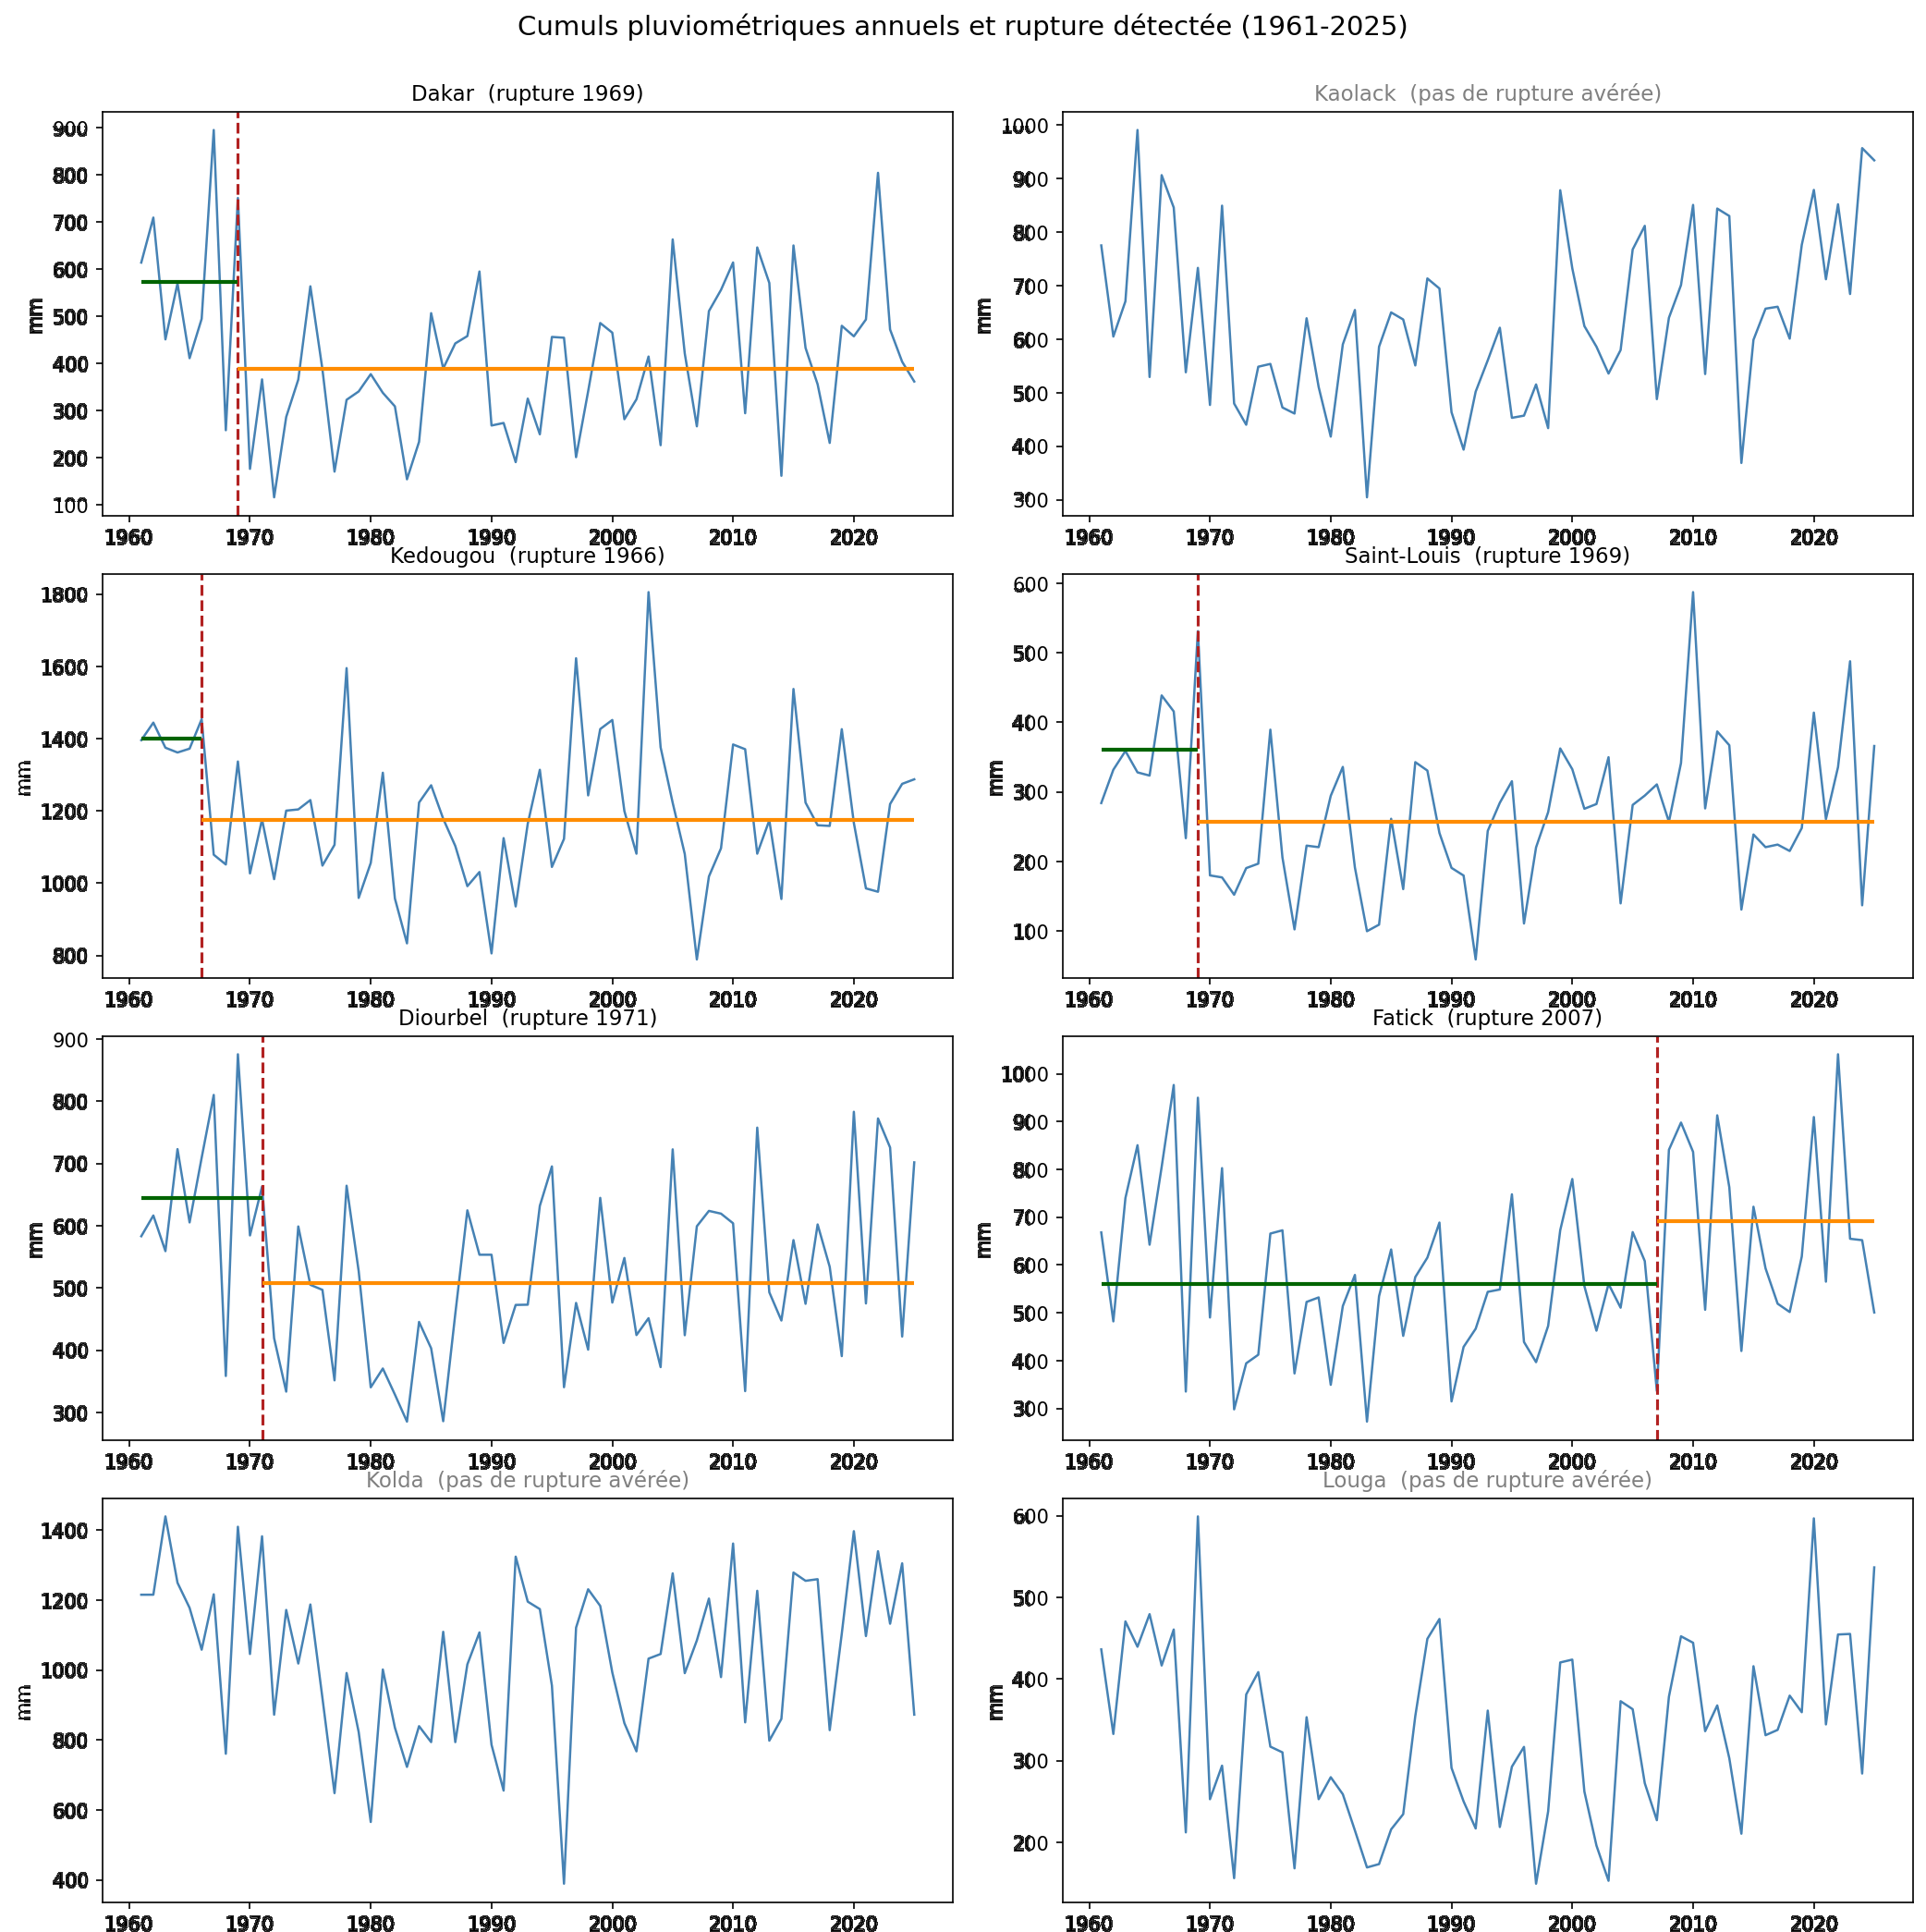
\includegraphics[width=\linewidth]{prism-uploads/graph1_series_ruptures_annexe_partie1.png}
\par\vspace{0.3cm}
\begin{center}
{\small\itshape Source : ANACIM, calculs de l’auteur.}
\end{center}
\end{figure}

\clearpage
\noindent{\annextitlefont ANNEXE A --- Suite}\par\medskip
\begin{figure}[H]
\ContinuedFloat
\centering
\caption[]{Séries pluviométriques régionales annuelles et ruptures détectées (1961-2025), suite : Sédhiou, Matam, Tambacounda, Thiès, Ziguinchor et Kaffrine}
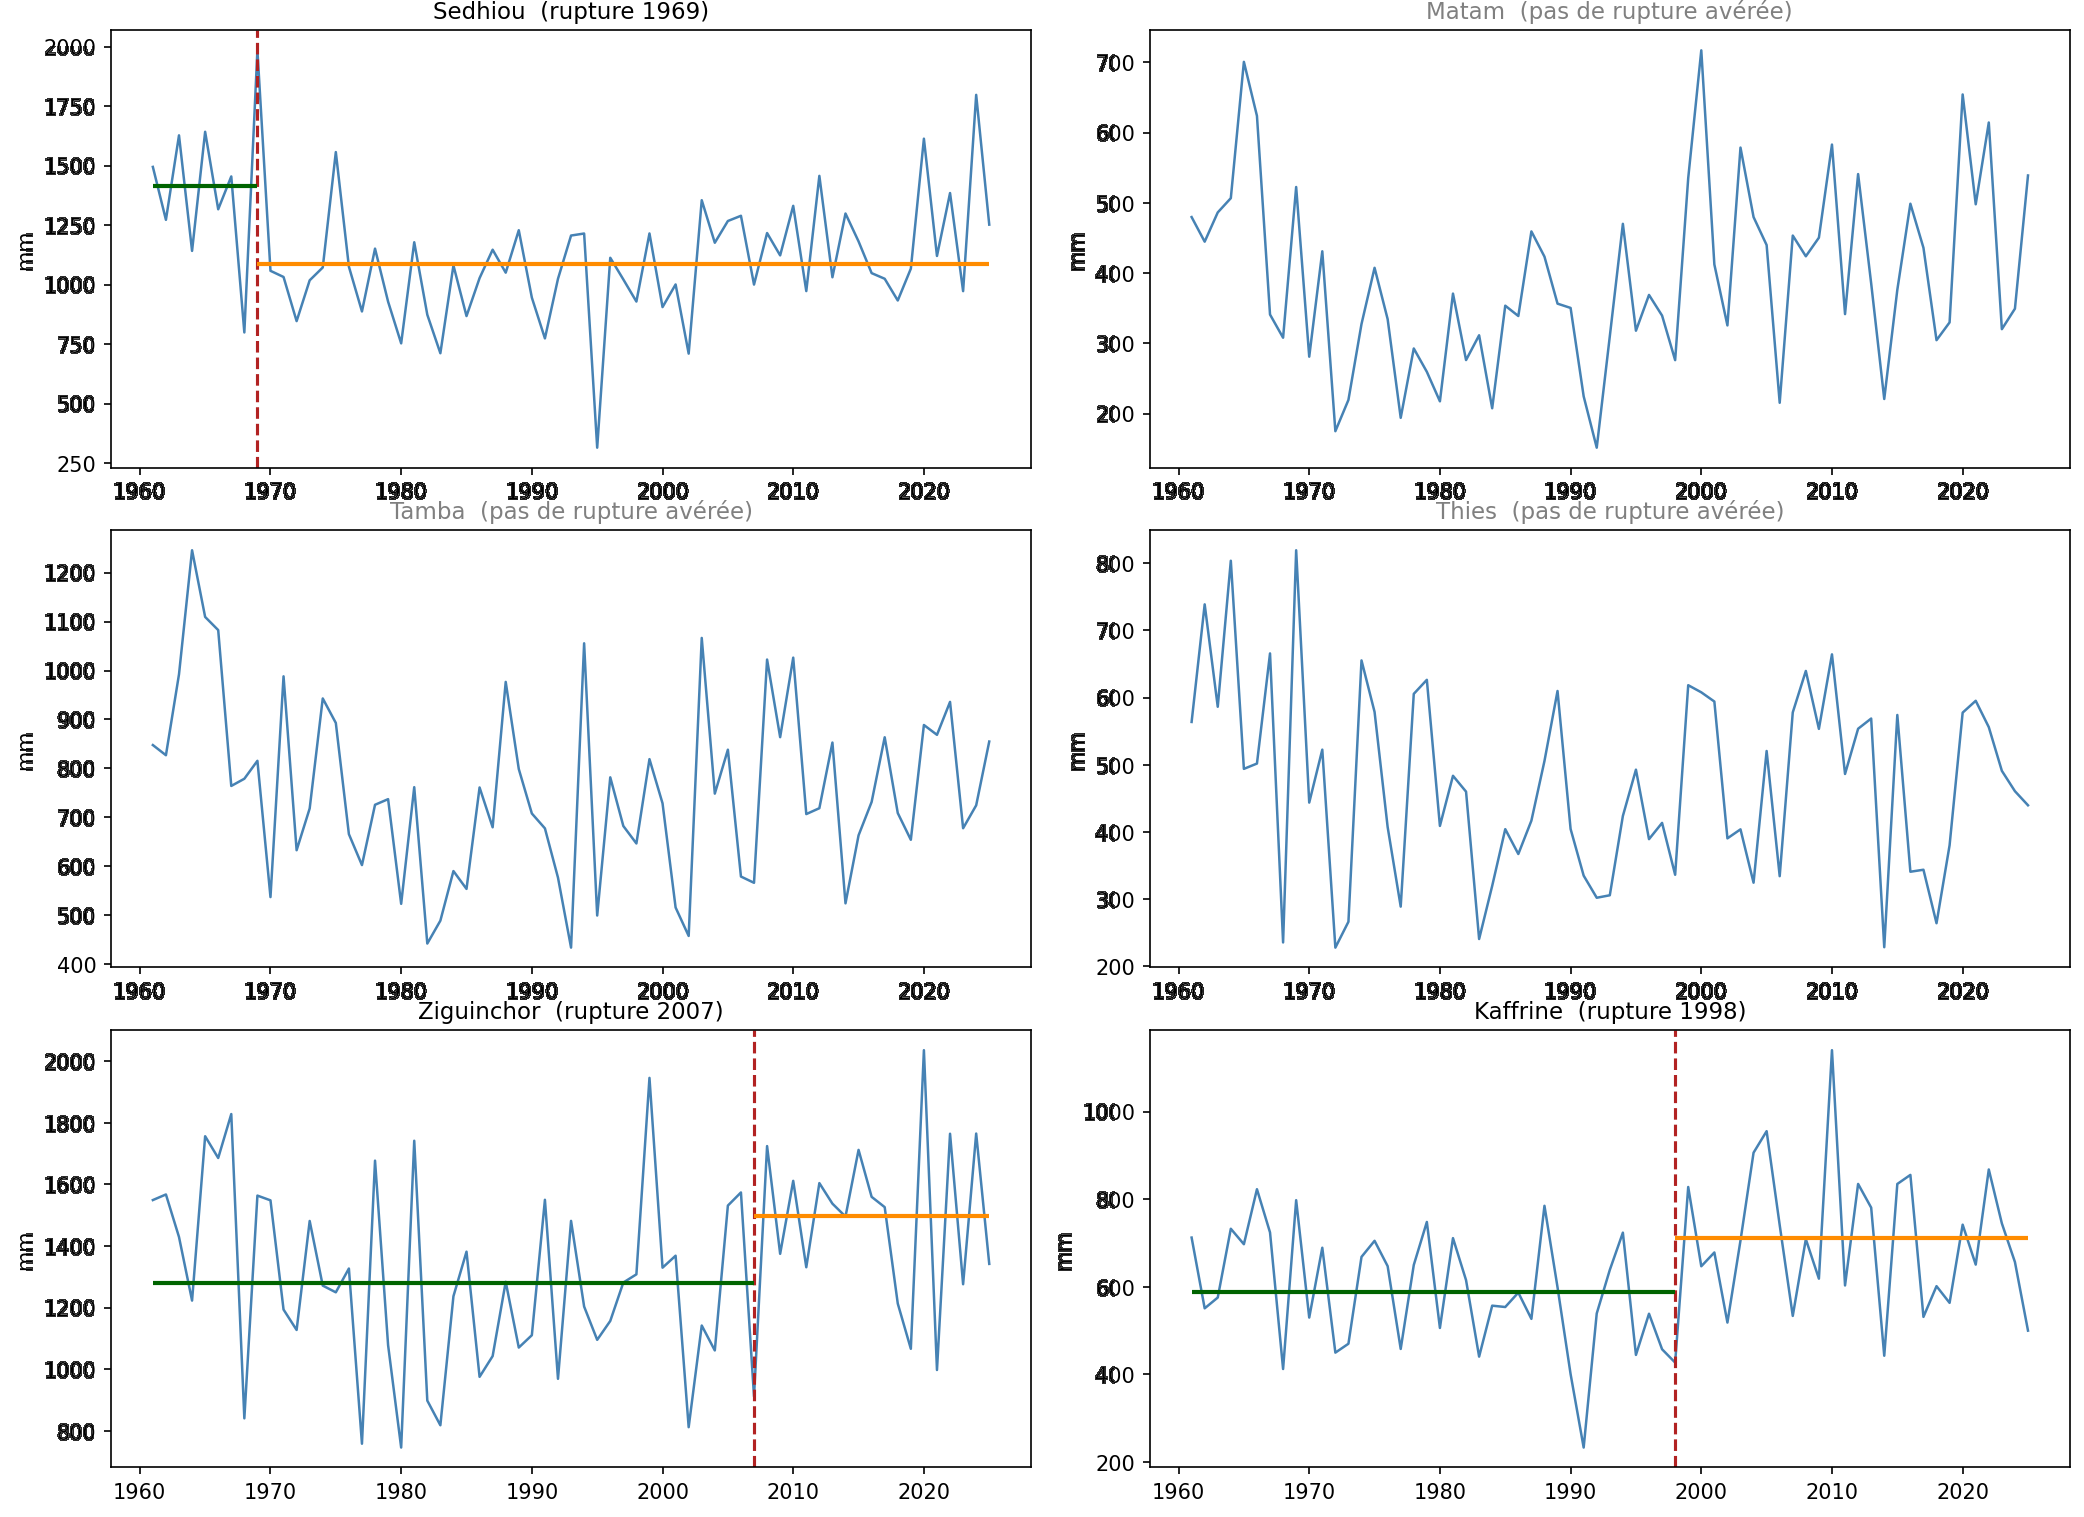
\includegraphics[width=\linewidth]{prism-uploads/graph1_series_ruptures_annexe_partie2.png}
\smallskip
\begin{minipage}{\linewidth}
\footnotesize
\textit{Lecture :} Les courbes bleues représentent les cumuls annuels en mm. Pour les régions présentant une rupture avérée, les segments vert et orange indiquent les moyennes avant et après rupture ; le trait rouge discontinu repère l'année de rupture. Les six autres régions sont signalées par la mention « pas de rupture avérée ».
\end{minipage}
\par\smallskip
\begin{center}
{\small\itshape Source : ANACIM, calculs de l’auteur.}
\end{center}
\end{figure}

\clearpage
\fancyhead[C]{\scriptsize\slshape ANNEXE B : INDICES PLUVIOMÉTRIQUES STANDARDISÉS RÉGIONAUX LISSÉS}
\markboth{ANNEXE B : INDICES PLUVIOMÉTRIQUES STANDARDISÉS RÉGIONAUX LISSÉS}{ANNEXE B}
\thispagestyle{fancy}
\noindent{\annextitlefont ANNEXE B}\par
\vspace{0.35em}{\color{navyblue}\titlerule[1.2pt]}\par\smallskip
\addcontentsline{toc}{chapter}{ANNEXE B : Indices pluviométriques standardisés régionaux lissés}
\setcounter{figure}{0}
\renewcommand{\thefigure}{B.\arabic{figure}}

\begin{figure}[H]
\centering
\captionsetup{justification=centering}
\caption{Indices pluviométriques standardisés lissés des quatorze régions du Sénégal (1961-2025)}
\label{fig:ips-lisses-regions-annexe}
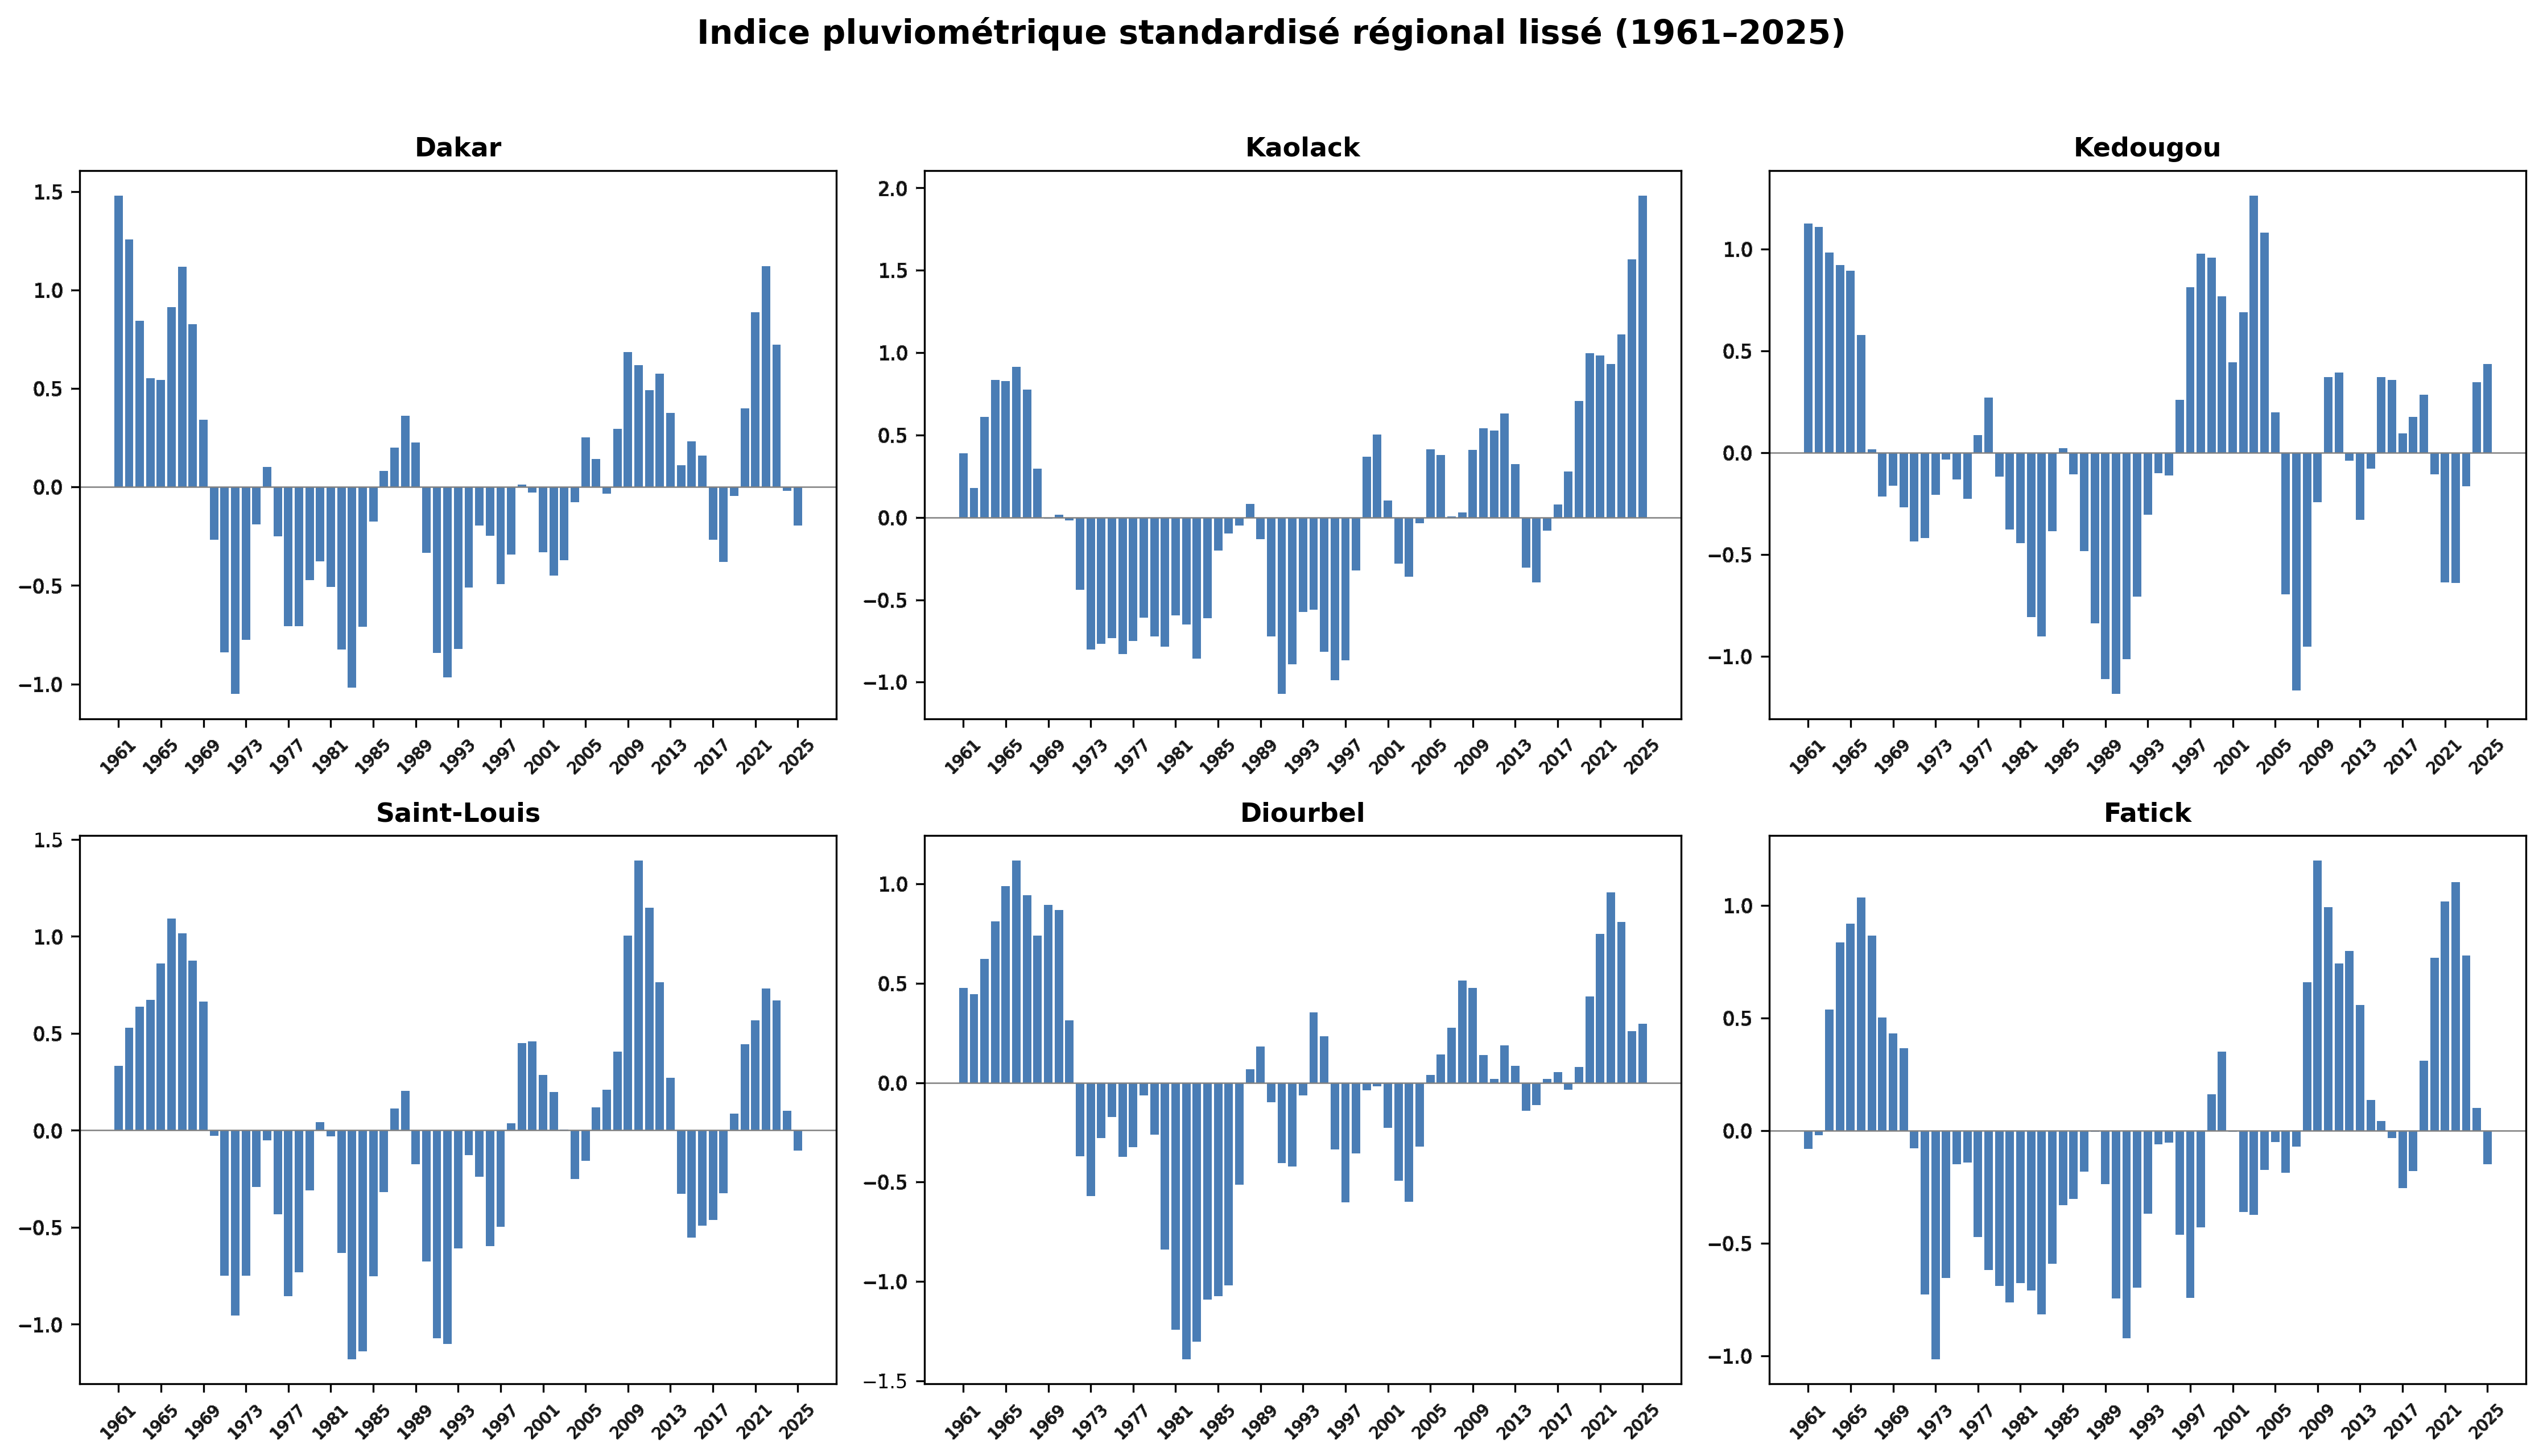
\includegraphics[width=0.86\linewidth]{prism-uploads/Annexe_IPS_regions_grille_partie1.png}
\par\smallskip
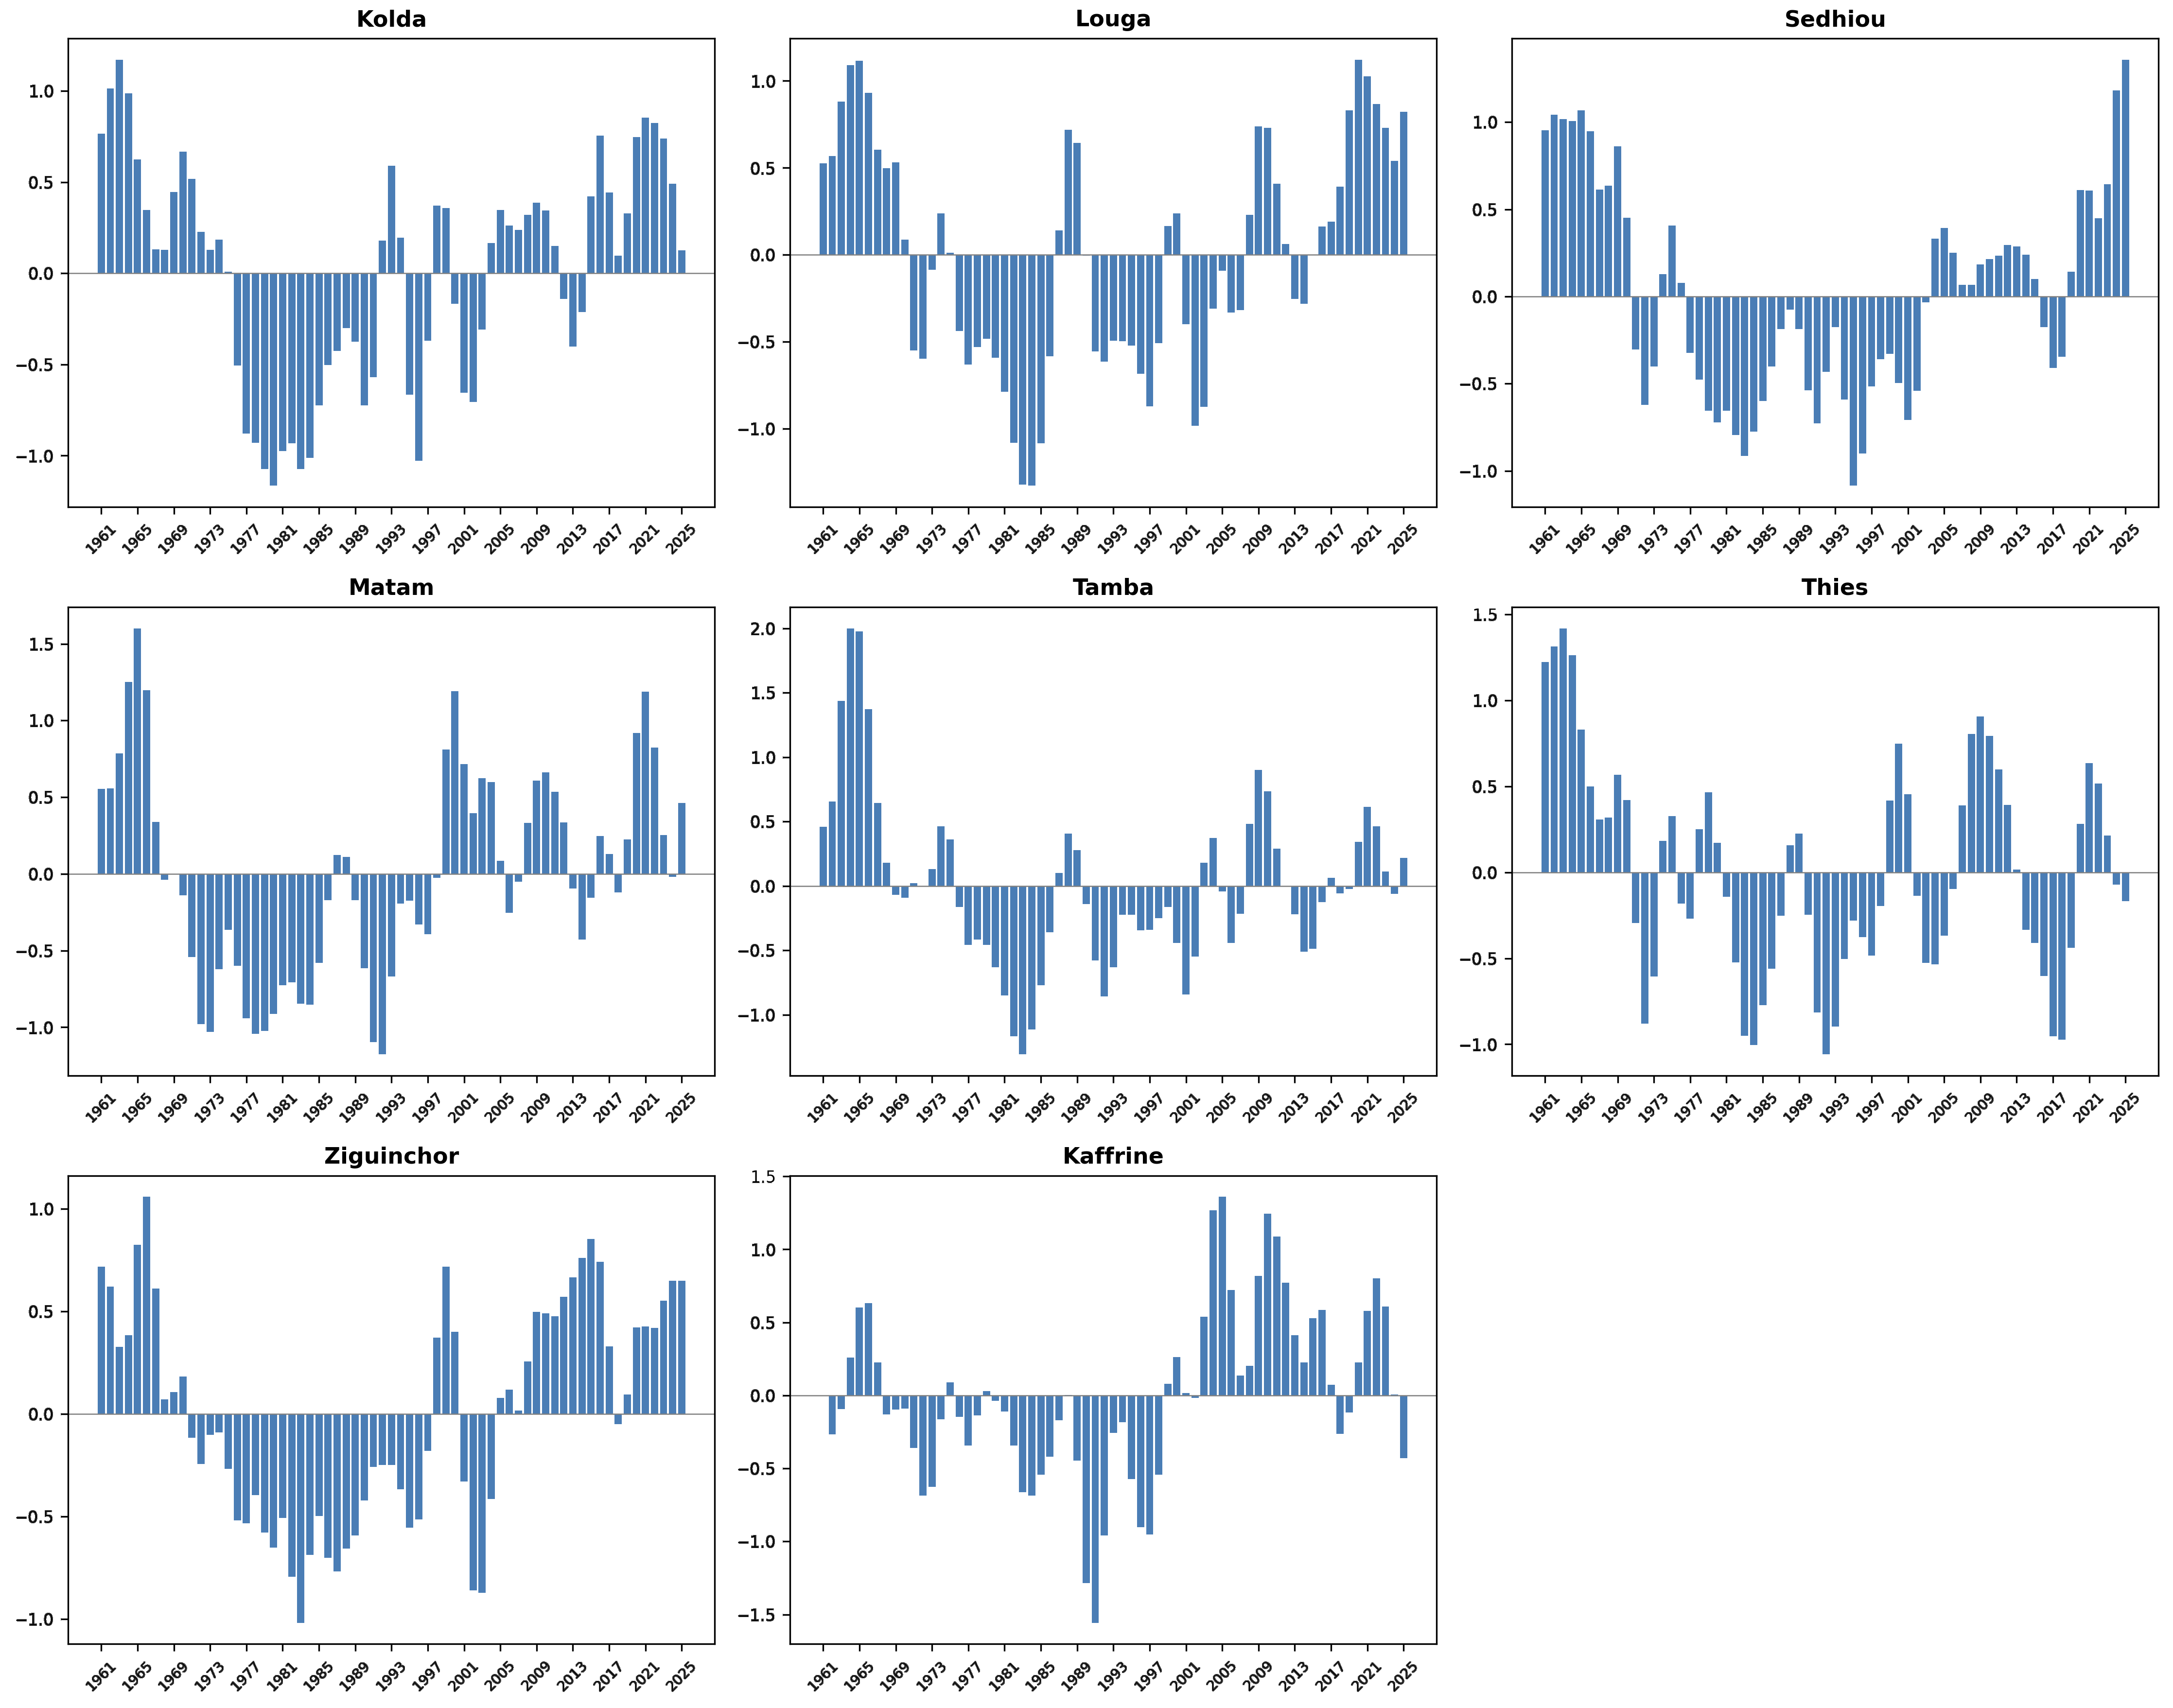
\includegraphics[width=0.86\linewidth]{prism-uploads/Annexe_IPS_regions_grille_partie2.png}
\par\smallskip
\begin{center}
{\small\itshape Source : ANACIM, calculs de l’auteur.}
\end{center}
\end{figure}

\clearpage
\fancyhead[C]{\scriptsize\slshape ANNEXE C : ORGANIGRAMME DE L'ANSD}
\begin{landscape}
\chapter*{ANNEXE C : Organigramme de l'ANSD}
\addcontentsline{toc}{chapter}{ANNEXE C : Organigramme de l'ANSD}
\markboth{ANNEXE C : ORGANIGRAMME DE L'ANSD}{ANNEXE C}
\thispagestyle{fancy}
\setcounter{figure}{0}
\renewcommand{\thefigure}{C.\arabic{figure}}

\vspace{-0.5cm}
\begin{center}
\captionof{figure}{Organigramme de l'Agence nationale de la Statistique et de la Démographie}
\label{fig:organigramme}
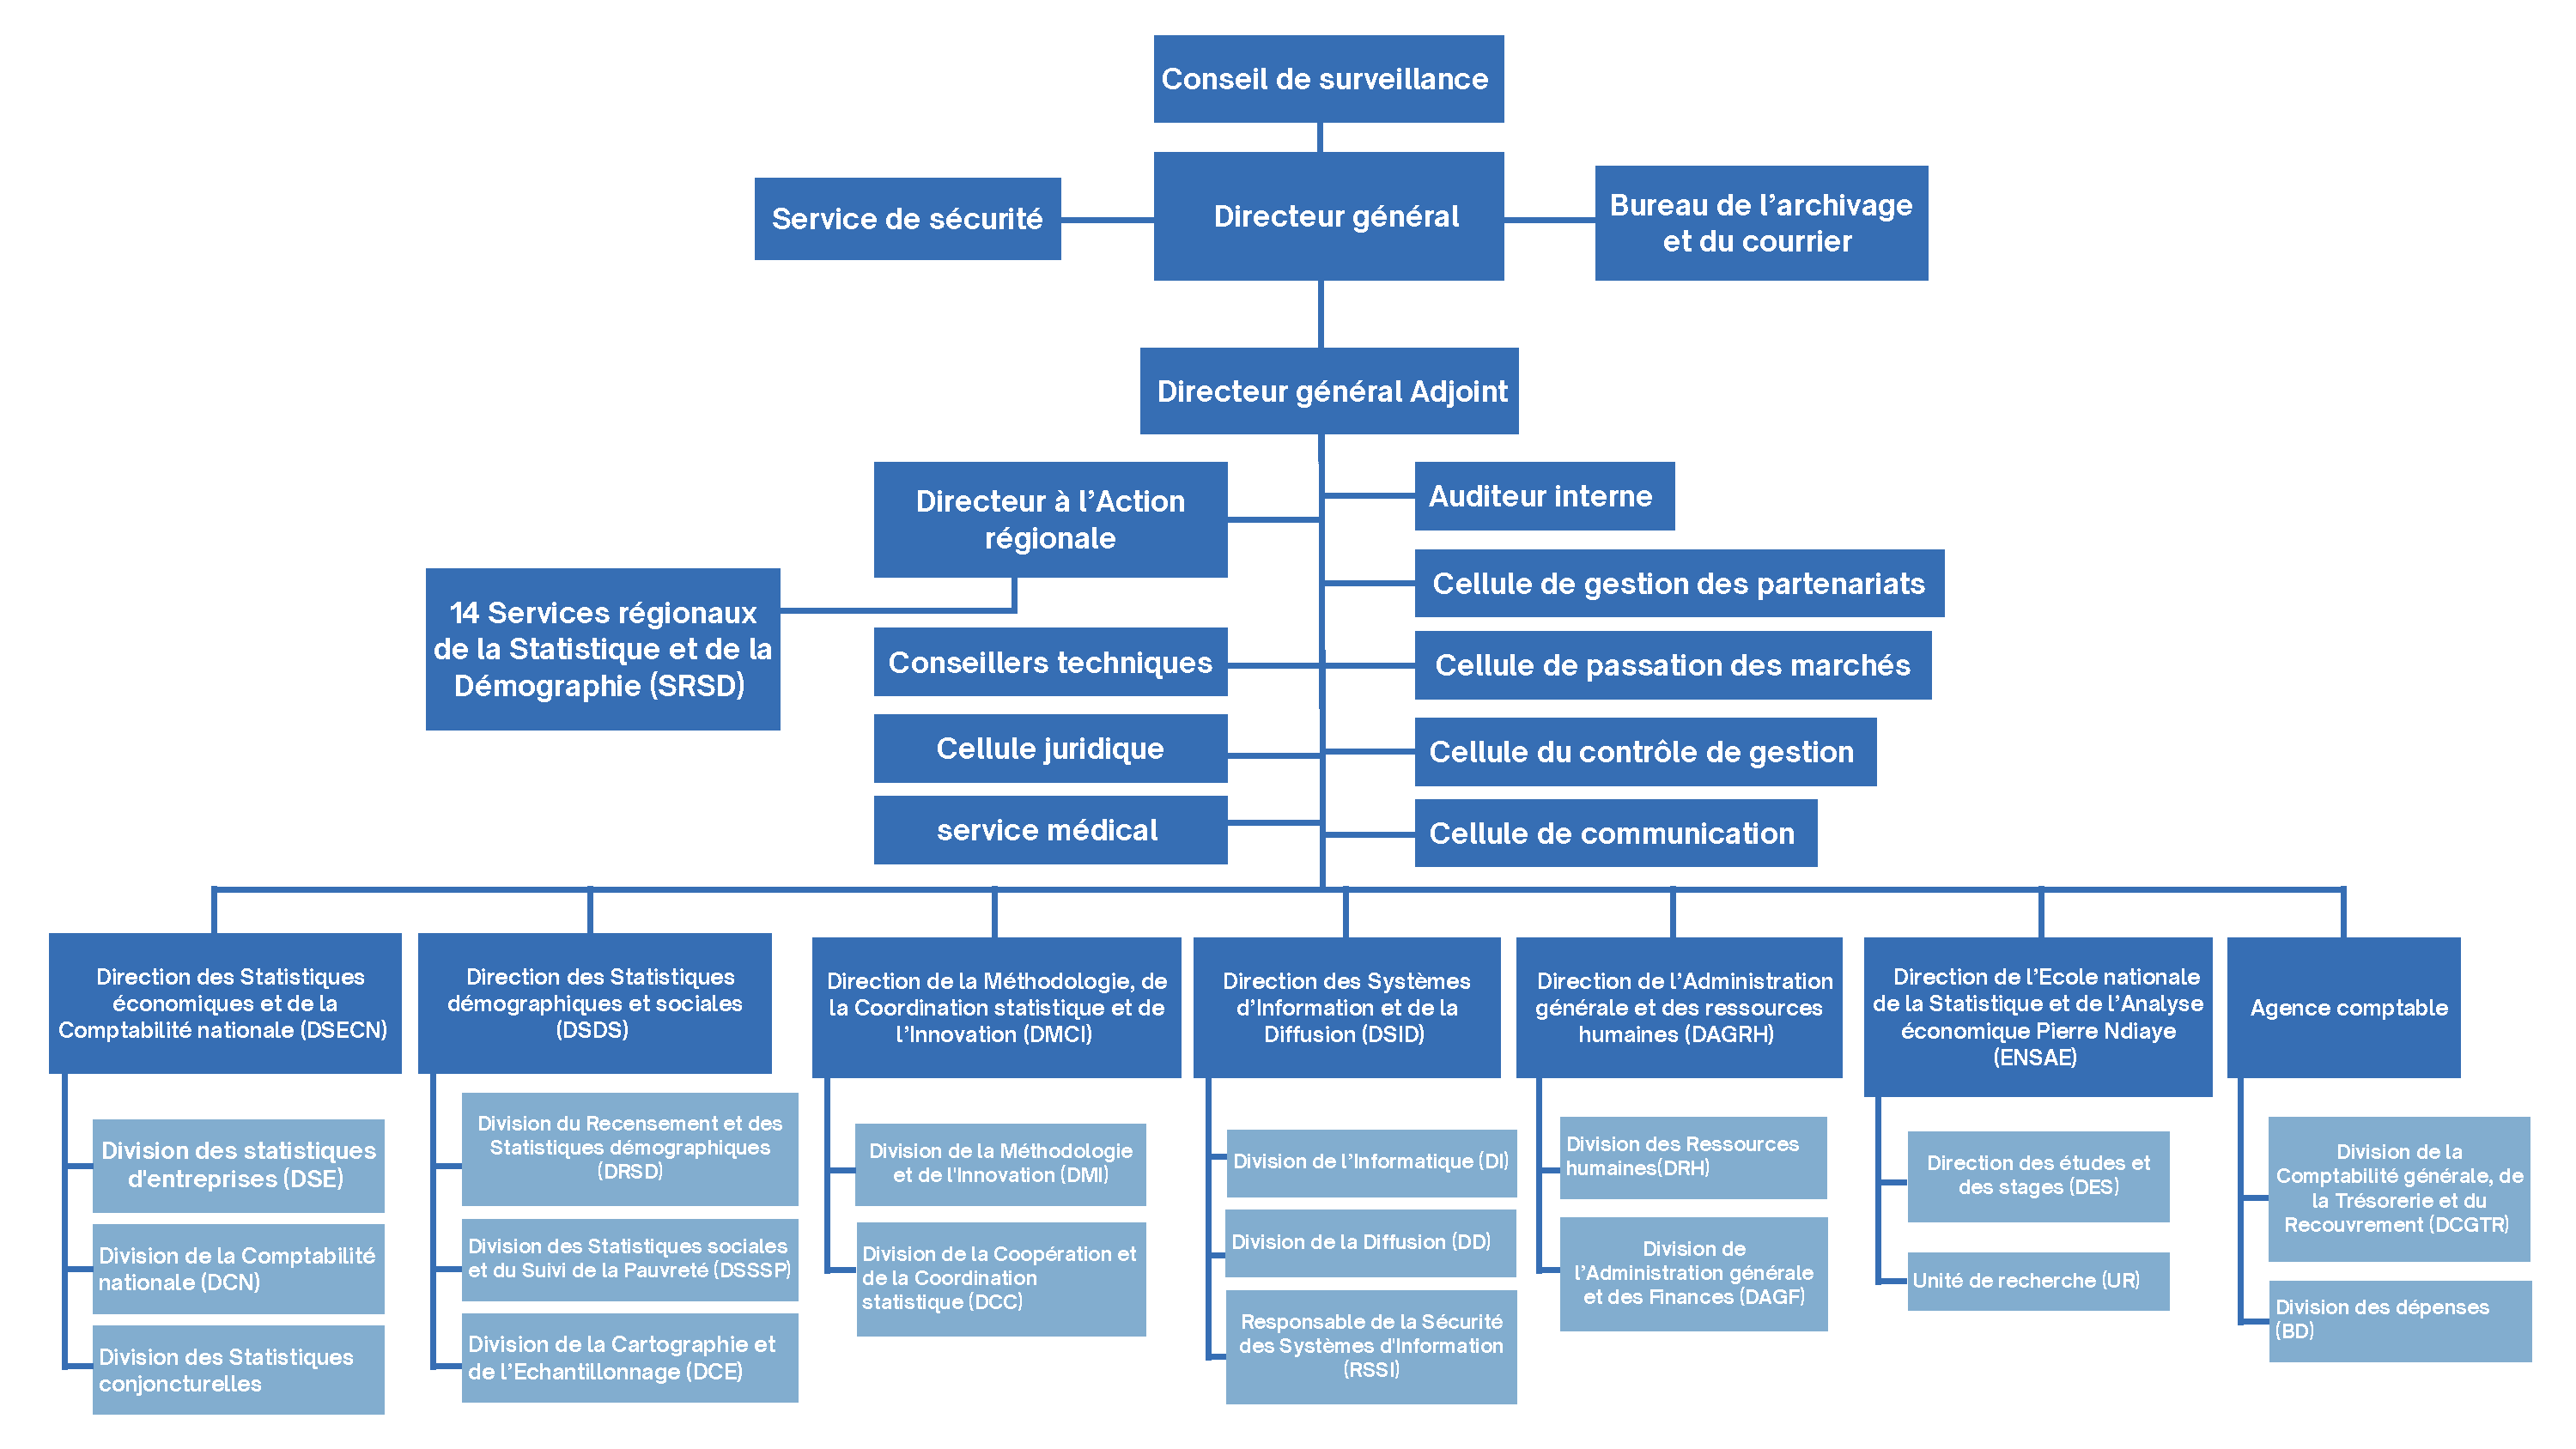
\includegraphics[
  width=0.78\linewidth,
  keepaspectratio
]{organigramme_ansd.pdf}

{\small\itshape Source : Agence nationale de la Statistique et de la Démographie (ANSD).}
\end{center}
\end{landscape}

% ===================== ANNEXE D =====================
\clearpage
\fancyhead[C]{\scriptsize\slshape ANNEXE D : MINIMA ET MAXIMA PLUVIOMÉTRIQUES DES QUATORZE RÉGIONS}
\chapter*{ANNEXE D}
\addcontentsline{toc}{chapter}{ANNEXE D : Minima et maxima pluviométriques des quatorze régions}
\markboth{ANNEXE D : MINIMA ET MAXIMA PLUVIOMÉTRIQUES DES QUATORZE RÉGIONS}{ANNEXE D}
\thispagestyle{fancy}
\setcounter{figure}{0}
\renewcommand{\thefigure}{D.\arabic{figure}}

\begin{figure}[H]
\centering
\captionsetup{justification=centering}
\caption{Cumuls pluviométriques annuels minimaux et maximaux des quatorze régions et années correspondantes}
\label{fig:extremes-pluviometriques-annexe}
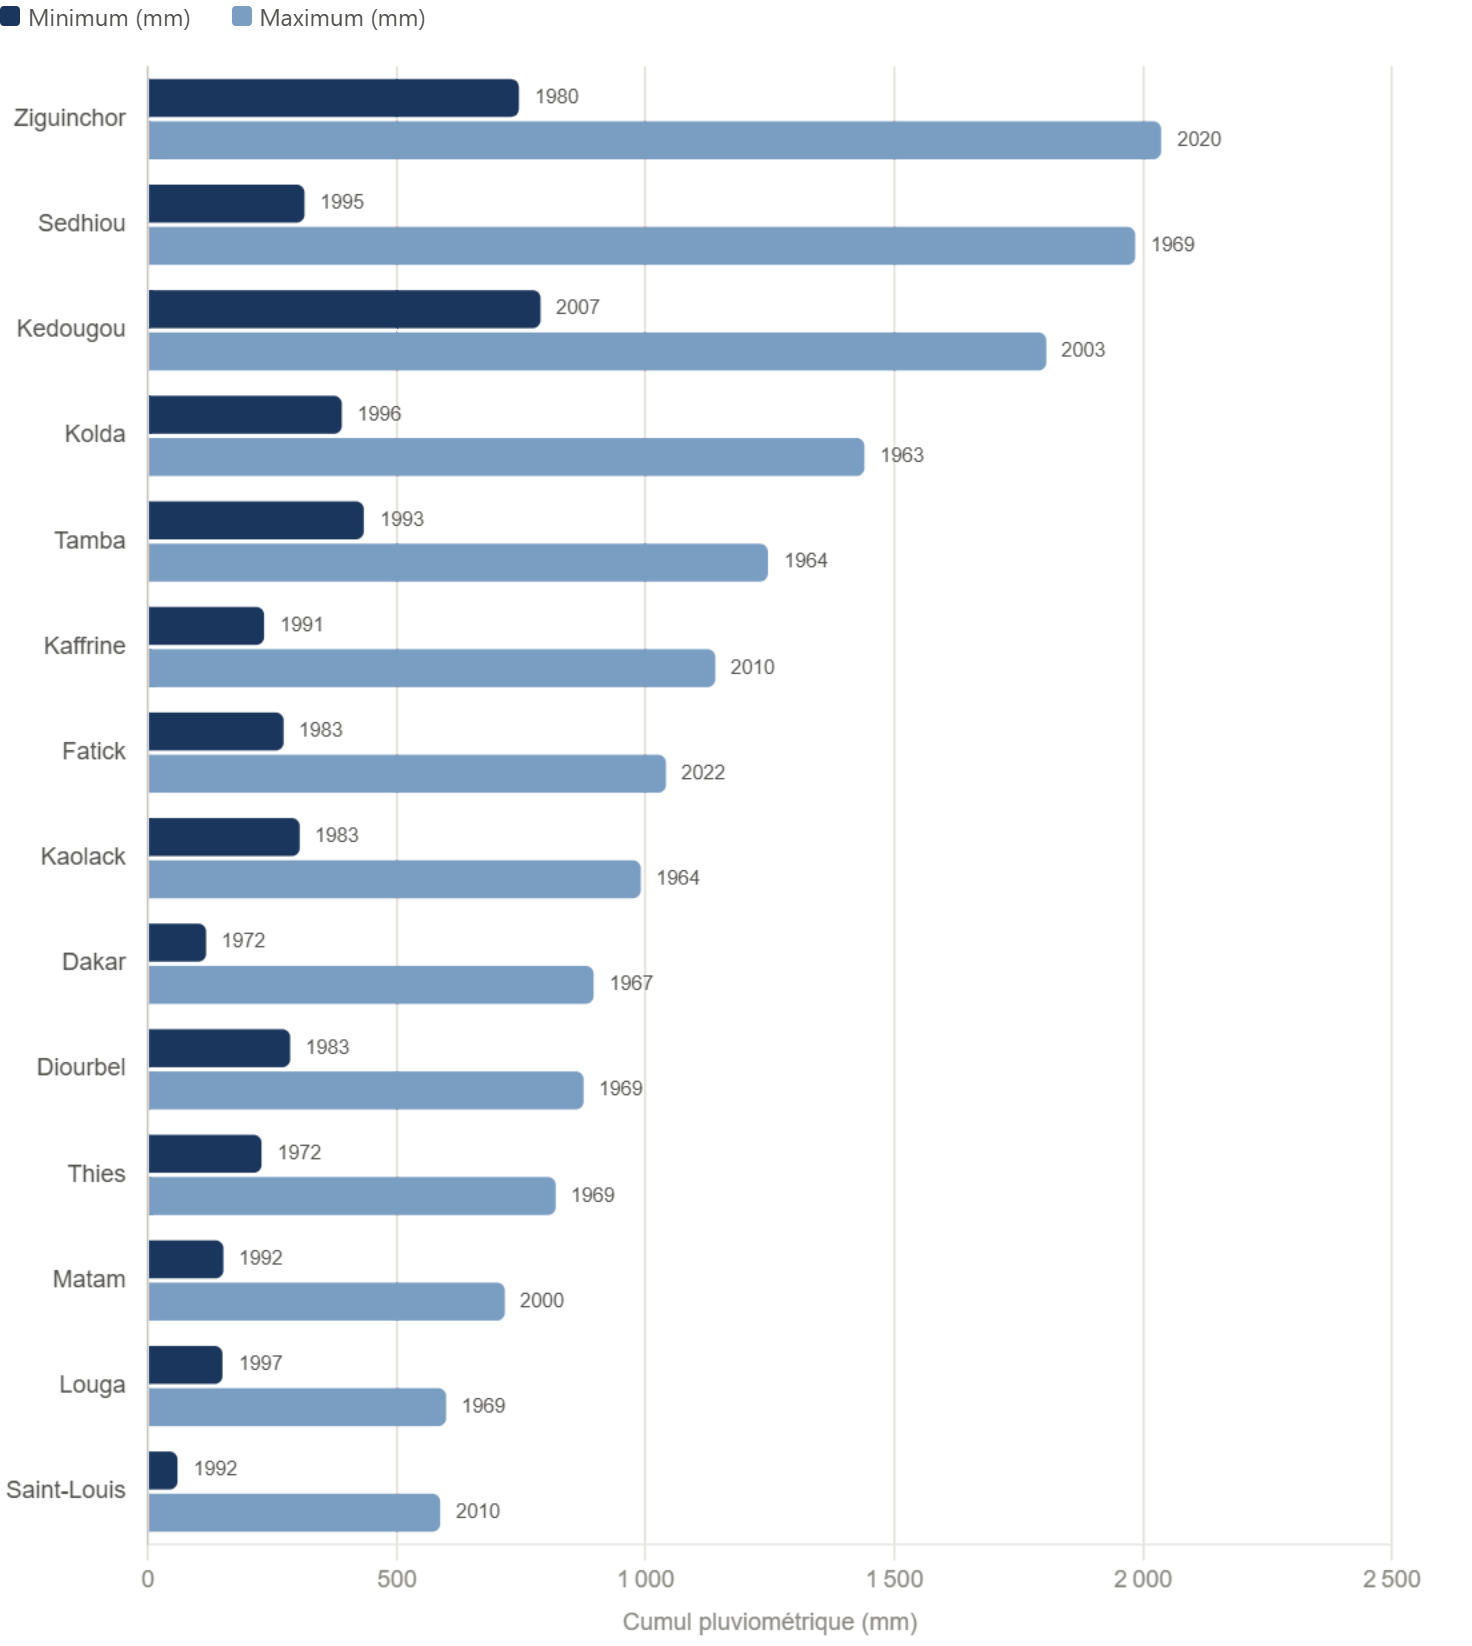
\includegraphics[width=0.95\linewidth,height=0.72\textheight,keepaspectratio]{prism-uploads/image_5_harmonisee.png}
\par\smallskip
\begin{center}
{\small\itshape Source : ANACIM, calculs de l’auteur.}
\end{center}
\end{figure}

% ===================== ANNEXE E =====================
\clearpage
\begin{landscape}
\fancyhead[C]{\scriptsize\slshape ANNEXE E : DENDROGRAMME DE LA CLASSIFICATION DES ANNÉES}
\noindent{\annextitlefont ANNEXE E : Dendrogramme de la classification des années}\par
\vspace{0.35em}{\color{navyblue}\titlerule[1.2pt]}\par\smallskip
\addcontentsline{toc}{chapter}{ANNEXE E : Dendrogramme de la classification des années}
\markboth{ANNEXE E : DENDROGRAMME DE LA CLASSIFICATION DES ANNÉES}{ANNEXE E}
\thispagestyle{fancy}
\setcounter{figure}{0}
\renewcommand{\thefigure}{E.\arabic{figure}}

\begin{figure}[H]
\centering
\captionsetup{justification=centering}
\caption{Dendrogramme de la classification ascendante hiérarchique des 65 années d'observation selon le critère de Ward}
\label{fig:dendrogramme-classification-annees}
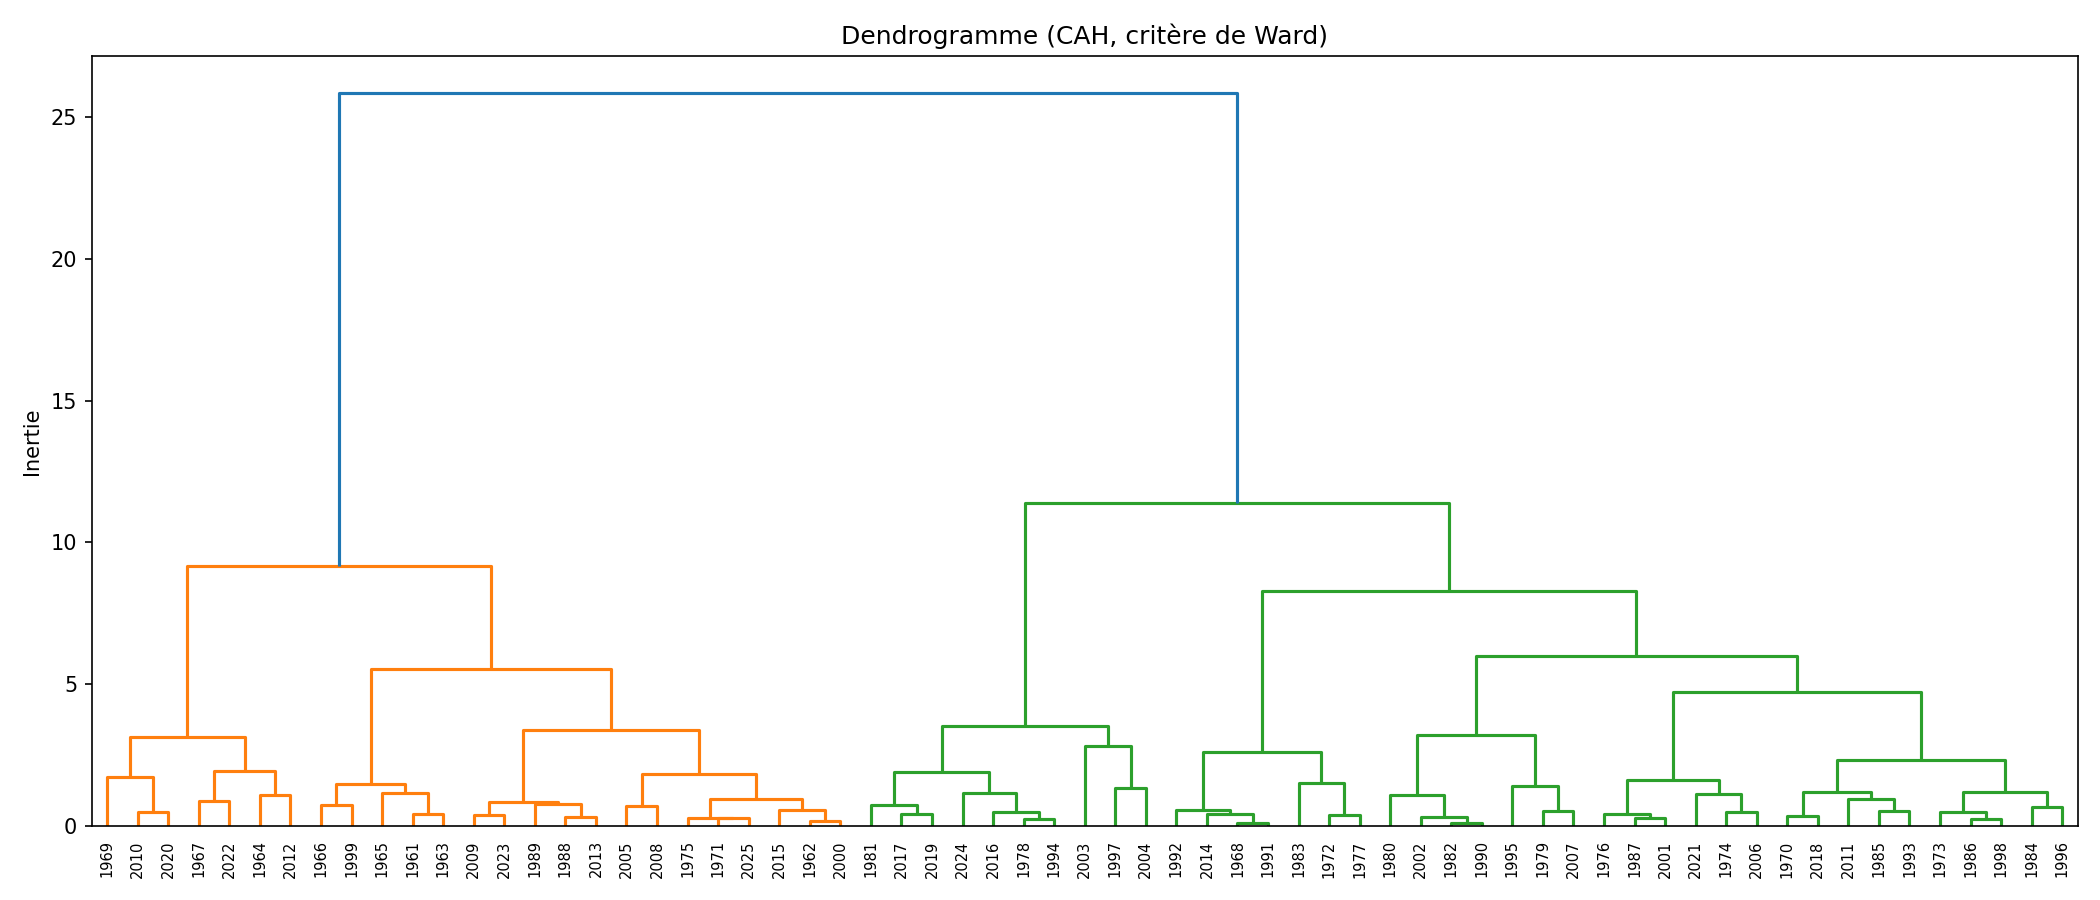
\includegraphics[width=\linewidth,keepaspectratio]{prism-uploads/graph7_dendrogramme.png}
\par\smallskip
\begin{center}
{\small\itshape Source : ANACIM, calculs de l’auteur.}
\end{center}
\end{figure}
\end{landscape}
\fancyhead[C]{\scriptsize\slshape \leftmark}

% ===================== ANNEXE F =====================
\clearpage
\markboth{ANNEXE F : ANALYSE DE SENSIBILITÉ DE LA TOLÉRANCE}{ANNEXE F}
\fancyhead[C]{\scriptsize\slshape ANNEXE F : ANALYSE DE SENSIBILITÉ DE LA TOLÉRANCE}
\thispagestyle{fancy}
\noindent{\annextitlefont ANNEXE F --- Analyse de sensibilité de la tolérance}\par
\addcontentsline{toc}{chapter}{ANNEXE F : Analyse de sensibilité de la tolérance}
\smallskip
{\renewcommand{\thetable}{F.\arabic{table}}%
\setcounter{table}{0}%
\begin{table}[H]
\centering
\captionsetup{justification=centering,font=small,labelfont=bf}
\caption{Sensibilité du nombre de régions à rupture avérée à la tolérance de concordance}
\label{tab:sensibilite-tolerance-ruptures}
\begingroup
\footnotesize
\renewcommand{\arraystretch}{1.2}
\begin{tabularx}{\linewidth}{>{\centering\arraybackslash}p{2.6cm}>{\centering\arraybackslash}p{3.1cm}>{\raggedright\arraybackslash}X}
\toprule
\rowcolor{navyblue}
\color{white}\textbf{Tolérance (ans)} &
\color{white}\textbf{Régions à rupture avérée} &
\multicolumn{1}{>{\centering\arraybackslash}X}{\color{white}\textbf{Régions}} \\
\midrule
\rowcolor{navyblue!6}
0 & 8 & Dakar, Kédougou, Saint-Louis, Diourbel, Fatick, Sédhiou, Ziguinchor et Kaffrine \\
1 & 8 & Identiques \\
\rowcolor{navyblue!6}
2 & 8 & Identiques \\
\rowcolor{navyblue!16}
\textbf{3 (retenue)} & \textbf{8} & \textbf{Identiques} \\
\rowcolor{navyblue!6}
4 & 10 & Les huit précédentes, plus Kolda et Thiès \\
5 & 10 & Identiques à la tolérance de 4 ans \\
\bottomrule
\end{tabularx}
\endgroup
\tablesource
\end{table}}
\fancyhead[C]{\scriptsize\slshape \leftmark}

% ===================== TABLE DES MATIÈRES FINALE =====================
\clearpage
\phantomsection
\addcontentsline{toc}{chapter}{TABLE DES MATIÈRES}
\renewcommand{\contentsname}{TABLE DES MATIÈRES}
% La table finale conserve le détail jusqu'aux sous-sous-sections.
\etocsetnexttocdepth{subsubsection}
\tableofcontents

\end{document}